% Consolidated manuscript: all text, TikZ figures, and tables are below.
% Shared bibliography: C:/mytex/svozil.bib; bibliography entries are not embedded.
% Edit this file directly; the former modular folders are retained only as provenance.
% Companion reference numbers are embedded, so no companion AUX file is required.
% Run the package build.py after changing labels or numbering in either manuscript.
\documentclass[aps,pra,reprint,superscriptaddress,longbibliography,nofootinbib,floatfix,10pt]{revtex4-2}
\usepackage[T1]{fontenc}
\usepackage{lmodern,amsmath,amssymb,amsthm,mathtools,bm,graphicx,booktabs,longtable,tikz,placeins,needspace,microtype}
\usetikzlibrary{calc,arrows.meta}
\usepackage[colorlinks=true,linkcolor=blue,citecolor=blue,urlcolor=blue,breaklinks=true]{hyperref}
\usepackage{orcidlink}
\newtheorem{theorem}{Theorem}
\newtheorem{lemma}[theorem]{Lemma}
\newtheorem{proposition}[theorem]{Proposition}
\newtheorem{corollary}[theorem]{Corollary}
\theoremstyle{definition}\newtheorem{definition}[theorem]{Definition}
\theoremstyle{remark}\newtheorem{remark}[theorem]{Remark}
\newcommand{\C}{\mathbb C}\newcommand{\R}{\mathbb R}\newcommand{\Q}{\mathbb Q}
\newcommand{\F}{\mathbb F}\newcommand{\Z}{\mathbb Z}\newcommand{\PP}{\mathbb P}
\newcommand{\Sc}{\mathcal S}\newcommand{\Cc}{\mathcal C}
\newcommand{\YO}{\mathrm{YO}}\newcommand{\ip}[2]{\langle #1,#2\rangle}
\DeclareMathOperator{\spanop}{span}\DeclareMathOperator{\rank}{rank}
\DeclareMathOperator{\diag}{diag}\DeclareMathOperator{\Tr}{Tr}\DeclareMathOperator{\tr}{tr}
\DeclareMathOperator{\supp}{supp}\DeclareMathOperator{\conv}{conv}
% BEGIN INLINED FILE: figures/yu-oh-styles.tex
% Symmetric Yu--Oh figure, adapted from Svozil (2025), Fig. 1(a).
\newif\ifDistinctContexts
\DistinctContextsfalse

% Constant colours on context orbits preserve the threefold colour symmetry.
\definecolor{YOtriad}{HTML}{246A9A}
\definecolor{YObasis}{HTML}{8A939B}
\definecolor{YOspoke}{HTML}{237D70}
\definecolor{YOouterA}{HTML}{85458B}
\definecolor{YOouterB}{HTML}{B47620}
\definecolor{YOdiagonal}{HTML}{B44850}
\colorlet{YOctx1}{YOtriad}
\colorlet{YOctx2}{YOtriad}
\colorlet{YOctx3}{YOtriad}
\colorlet{YOctx4}{YObasis}
\colorlet{YOctx5}{YOspoke}
\colorlet{YOctx6}{YOspoke}
\colorlet{YOctx7}{YOspoke}
\colorlet{YOctx8}{YOouterA}
\colorlet{YOctx11}{YOouterA}
\colorlet{YOctx16}{YOouterA}
\colorlet{YOctx9}{YOouterB}
\colorlet{YOctx13}{YOouterB}
\colorlet{YOctx14}{YOouterB}
\colorlet{YOctx10}{YOdiagonal}
\colorlet{YOctx12}{YOdiagonal}
\colorlet{YOctx15}{YOdiagonal}
\ifDistinctContexts
  \definecolor{YOctx1}{HTML}{BF1FB4}
  \definecolor{YOctx2}{HTML}{B4000A}
  \definecolor{YOctx3}{HTML}{C99400}
  \definecolor{YOctx4}{HTML}{555F00}
  \definecolor{YOctx5}{HTML}{559F2A}
  \definecolor{YOctx6}{HTML}{D48A6A}
  \definecolor{YOctx7}{HTML}{F47400}
  \definecolor{YOctx8}{HTML}{B4944A}
  \definecolor{YOctx9}{HTML}{DF74BF}
  \definecolor{YOctx10}{HTML}{744ABF}
  \definecolor{YOctx11}{HTML}{35552A}
  \definecolor{YOctx12}{HTML}{C955FF}
  \definecolor{YOctx13}{HTML}{00B49F}
  \definecolor{YOctx14}{HTML}{6A558A}
  \definecolor{YOctx15}{HTML}{743F00}
  \definecolor{YOctx16}{HTML}{FF0035}
\fi
\tikzset{
  YOtrace/.style={line width=1.85pt,line cap=round,line join=round},
  YOapex/.style={line width=.68pt,line cap=round,draw opacity=.65},
  YOlabel/.style={font=\small,inner sep=1.2pt,fill=white},
  YOnumber/.style={font=\sffamily\bfseries\fontsize{8}{8}\selectfont,inner sep=0pt},
}
\newcommand{\YOline}[4]{\draw[YOtrace,YOctx#1] (v#2)--(v#3)--(v#4);}
\newcommand{\YOapexlink}[6]{%
  \draw[YOapex,draw=YOctx#1] (#3)
    -- ($(#3)!-#4!(#2)$)
    .. controls ($(#3)!-#5!(#2)$) and #6 .. (v26);%
}
\newcommand{\YOapexvia}[9]{%
  \draw[YOapex,draw=YOctx#1] (#3)
    -- ($(#3)!-#4!(#2)$)
    .. controls ($(#3)!-#5!(#2)$) and #6 .. #7
    .. controls #8 and #9 .. (v26);%
}
\newcommand{\YOvertex}[2]{%
  \foreach \context/\radius in {#2}{%
    \fill[YOctx\context] (v#1) circle[radius=\radius cm];%
  }%
  \fill[white] (v#1) circle[radius=.18cm];%
  \node[YOnumber] at (v#1) {#1};%
}
% END INLINED FILE: figures/yu-oh-styles.tex

% BEGIN INLINED FILE: figures/hesse37-figure-styles.tex
% Visual conventions copied from C:/mytex/2026-chroma-dim4-example.tex.
% Context colors identify contexts, not a proper vertex coloring.
\definecolor{ucA01}{HTML}{1C638E}
\definecolor{ucA02}{HTML}{257D72}
\definecolor{ucA03}{HTML}{BC681D}
\definecolor{ucA04}{HTML}{8B3D88}
\definecolor{ucA05}{HTML}{82623E}
\definecolor{ucA06}{HTML}{0000FF}
\definecolor{ucA07}{HTML}{00B400}
\definecolor{ucA08}{HTML}{FF15F4}
\definecolor{ucA09}{HTML}{FF005F}
\definecolor{ucA10}{HTML}{006AFF}
\definecolor{ucA11}{HTML}{8A9400}
\definecolor{ucA12}{HTML}{FF3500}
\definecolor{ucA13}{HTML}{E97F94}
\definecolor{ucA14}{HTML}{005F0A}
\definecolor{ucA15}{HTML}{FF4AB4}
\definecolor{ucA16}{HTML}{740AB4}
\definecolor{ucA17}{HTML}{6A9FFF}
\definecolor{ucA18}{HTML}{941F2A}
\definecolor{ucA19}{HTML}{C97FFF}
\definecolor{ucA20}{HTML}{00B474}
\definecolor{ucA21}{HTML}{7F9F5F}
\definecolor{ucA22}{HTML}{B494C9}
\definecolor{ucA23}{HTML}{2A4A9F}
\definecolor{ucA24}{HTML}{FF6A55}
\definecolor{sgink}{HTML}{3D454B}
\definecolor{sggray}{HTML}{858B90}
\tikzset{
 sg/context/.style={line width=1.15pt,line cap=round,line join=round,draw=sggray},
 sg/base/.style={line width=1.7pt,line cap=round,line join=round},
 sg/label/.style={font=\sffamily\small,text=sgink,fill=white,inner sep=1pt},
 sg/number/.style={inner sep=0pt,outer sep=0pt,text=black,
   font=\sffamily\fontsize{8}{8}\selectfont},
}
\newcommand{\HesseFCvertex}[2]{%
  \foreach \diskcolor/\diskradius in {#2}{%
    \fill[\diskcolor] (v#1) circle[radius=\diskradius cm];%
  }%
  \fill[white] (v#1) circle[radius=.160cm];%
  \node[sg/number] at (v#1) {#1};%
}
% END INLINED FILE: figures/hesse37-figure-styles.tex

% BEGIN INLINED FILE: figures/chromatic-context-diagrams.tex
% Reusable TikZ diagrams for H17,10 and H21,13 in the conventional
% Specker-bug hexagon layout. Yu--Oh vertex labels, context colours,
% thick traces, and concentric incidence rings are retained.
\providecommand{\CScontext}[4]{%
  \ifnum#1=4\relax
    % Context 4: one smooth, closed threefold curve through precisely v2,v8,v5.
    \pgfmathsetmacro{\YObasisR}{\YOR*cos(20)}%
    \foreach \rotation in {0,120,240}{%
      \begin{scope}[rotate=\rotation]
        \draw[YOtrace,YOctx4]
          (0,\YObasisR)
          .. controls ({-.5*\YObasisR},\YObasisR)
          and ({-(sqrt(3)/2+.25)*\YObasisR},{(-.5+.25*sqrt(3))*\YObasisR})
          .. ({-sqrt(3)/2*\YObasisR},{-.5*\YObasisR});
      \end{scope}%
    }%
  \else
    \YOline{#1}{#2}{#3}{#4}%
  \fi
}
\newcommand{\CSbasecontexts}{%
  \CScontext{1}{3}{2}{1}
  \CScontext{2}{9}{8}{7}
  \CScontext{3}{4}{5}{6}
  \CScontext{4}{2}{5}{8}
  \CScontext{8}{11}{14}{3}
  \CScontext{9}{7}{15}{11}
  \CScontext{10}{4}{24}{11}
  \CScontext{11}{9}{23}{10}
  \CScontext{12}{1}{19}{10}
  \CScontext{13}{10}{18}{4}
}
\newcommand{\CSaddedcontexts}{%
  \CScontext{14}{1}{20}{13}
  \CScontext{15}{7}{21}{13}
  \CScontext{16}{6}{22}{13}
}
% Nested context-colour rings for H17,10 (drawn after all traces).
\newcommand{\CSHseventeenvertices}{%
  \YOvertex{1}{1/.36,12/.27}
  \YOvertex{2}{1/.36,4/.27}
  \YOvertex{3}{1/.36,8/.27}
  \YOvertex{4}{3/.45,10/.36,13/.27}
  \YOvertex{5}{3/.36,4/.27}
  \YOvertex{6}{3/.27}
  \YOvertex{7}{2/.36,9/.27}
  \YOvertex{8}{2/.36,4/.27}
  \YOvertex{9}{2/.36,11/.27}
  \YOvertex{10}{11/.45,13/.36,12/.27}
  \YOvertex{11}{8/.45,9/.36,10/.27}
  \YOvertex{14}{8/.27}
  \YOvertex{15}{9/.27}
  \YOvertex{18}{13/.27}
  \YOvertex{19}{12/.27}
  \YOvertex{23}{11/.27}
  \YOvertex{24}{10/.27}
}
% Nested context-colour rings for H21,13 (drawn after all traces).
\newcommand{\CSHtwentyonevertices}{%
  \YOvertex{1}{1/.45,12/.36,14/.27}
  \YOvertex{2}{1/.36,4/.27}
  \YOvertex{3}{1/.36,8/.27}
  \YOvertex{4}{3/.45,10/.36,13/.27}
  \YOvertex{5}{3/.36,4/.27}
  \YOvertex{6}{3/.36,16/.27}
  \YOvertex{7}{2/.45,15/.36,9/.27}
  \YOvertex{8}{2/.36,4/.27}
  \YOvertex{9}{2/.36,11/.27}
  \YOvertex{10}{11/.45,13/.36,12/.27}
  \YOvertex{11}{8/.45,9/.36,10/.27}
  \YOvertex{13}{16/.45,14/.36,15/.27}
  \YOvertex{14}{8/.27}
  \YOvertex{15}{9/.27}
  \YOvertex{18}{13/.27}
  \YOvertex{19}{12/.27}
  \YOvertex{20}{14/.27}
  \YOvertex{21}{15/.27}
  \YOvertex{22}{16/.27}
  \YOvertex{23}{11/.27}
  \YOvertex{24}{10/.27}
}
\newcommand{\CSdrawcontextdiagram}[1]{%
  \begin{tikzpicture}[x=1cm,y=1cm]
    % All contexts in this layout are straight; the original curved
    % CScontext convention remains available to other figure macros.
    \let\CScontext\YOline
    % The six sides and vertical crossbar are precisely the 13-ray bug.
    \def\Rbug{4.4}%
    \coordinate (v10) at (0:\Rbug);
    \coordinate (v1) at (60:\Rbug);
    \coordinate (v3) at (120:\Rbug);
    \coordinate (v11) at (180:\Rbug);
    \coordinate (v7) at (240:\Rbug);
    \coordinate (v9) at (300:\Rbug);
    \coordinate (v2) at ($(v1)!.5!(v3)$);
    \coordinate (v8) at ($(v7)!.5!(v9)$);
    \coordinate (v5) at (0,0);
    \foreach \vertex/\first/\last in {14/3/11,15/11/7,23/9/10,19/10/1}{%
      \coordinate (v\vertex) at ($(v\first)!.5!(v\last)$);
    }
    % The three extra contexts of H17; none passes through an unrelated node.
    \coordinate (v4) at (-2.30,-.90);
    \ifnum#1=17\relax
      \coordinate (v6) at ($(v4)!.60!(v5)$);
    \else
      \coordinate (v6) at (1.38,.54);
    \fi
    \coordinate (v24) at ($(v11)!.52!(v4)$);
    \coordinate (v18) at ($(v10)!.42!(v4)$);
    % H21 adds the third diagonal sector above the common bug hexagon.
    \coordinate (v13) at (0,6.0);
    \coordinate (v20) at ($(v13)!.45!(v1)$);
    \coordinate (v22) at ($(v13)!.50!(v6)$);
    \coordinate (v21) at ($(v13)!.27!(v7)$);
    \CSbasecontexts
    \ifnum#1=21\relax
      \CSaddedcontexts
      \CSHtwentyonevertices
    \else
      \CSHseventeenvertices
    \fi
    % Supplementary Yu--Oh labels, with all original numbers retained.
    \node[YOlabel,left=4pt] at ($(v11)+(-.45,0)$) {$h_1$};
    \node[YOlabel,right=4pt] at ($(v10)+(.45,0)$) {$h_2$};
    \node[YOlabel,above=4pt] at ($(v3)+(0,.34)$) {$y_1^-$};
    \node[YOlabel,above=4pt] at ($(v1)+(0,.34)$) {$y_1^+$};
    \node[YOlabel,below=4pt] at ($(v7)+(0,-.34)$) {$y_2^+$};
    \node[YOlabel,below=4pt] at ($(v9)+(0,-.34)$) {$y_2^-$};
    \ifnum#1=17\relax
      \node[YOlabel,above=3pt] at ($(v4)+(0,.55)$) {$y_3^+$};
      \node[YOlabel,above=3pt] at ($(v6)+(0,.32)$) {$y_3^-$};
      \node[YOlabel,above=3pt] at ($(v2)+(0,.45)$) {$z_1$};
      \node[YOlabel,below=3pt] at ($(v8)+(0,-.45)$) {$z_2$};
      \node[YOlabel,right=3pt] at ($(v5)+(.40,0)$) {$z_3$};
    \else
      \node[YOlabel,left=3pt] at ($(v4)+(-.28,-.10)$) {$y_3^+$};
      \node[YOlabel,right=3pt] at ($(v6)+(.28,.10)$) {$y_3^-$};
      \node[YOlabel,left=3pt] at ($(v2)+(-.30,0)$) {$z_1$};
      \node[YOlabel,right=3pt] at ($(v8)+(.30,0)$) {$z_2$};
      \node[YOlabel,right=3pt] at ($(v5)+(.28,-.30)$) {$z_3$};
    \fi
    \ifnum#1=21\relax
      \node[YOlabel,above=4pt] at ($(v13)+(0,.40)$) {$h_3$};
    \fi
    % Equal frames preserve the common positions in the two restrictions.
    \pgfresetboundingbox
    \path[use as bounding box] (-6.52,-4.90) rectangle (6.52,7.0);
  \end{tikzpicture}%
}
% END INLINED FILE: figures/chromatic-context-diagrams.tex

% BEGIN INLINED FILE: figures/chromatic-gadgets-3d.tex
% Macros copied verbatim from chromatic-tifs-tits-standalone.tex.
\tikzset{
  CSexcl/.style={draw=YOdiagonal,line width=1.6pt,densely dashed,{Latex[length=2.4mm]}-{Latex[length=2.4mm]}},
  CSident/.style={draw=YOtriad,line width=1.6pt,densely dotted,{Latex[length=2.4mm]}-{Latex[length=2.4mm]}},
  CSnote/.style={font=\sffamily\footnotesize,fill=white,inner sep=1.5pt,rounded corners=1pt},
  CSvec/.style={font=\scriptsize,text=black!75,inner sep=1pt},
}

% (a) Pentagon P_5: 3-ary purely chromatic TIFS on {6,7,9} with integer FOR in R^3
\newcommand{\CSdrawPfive}{%
  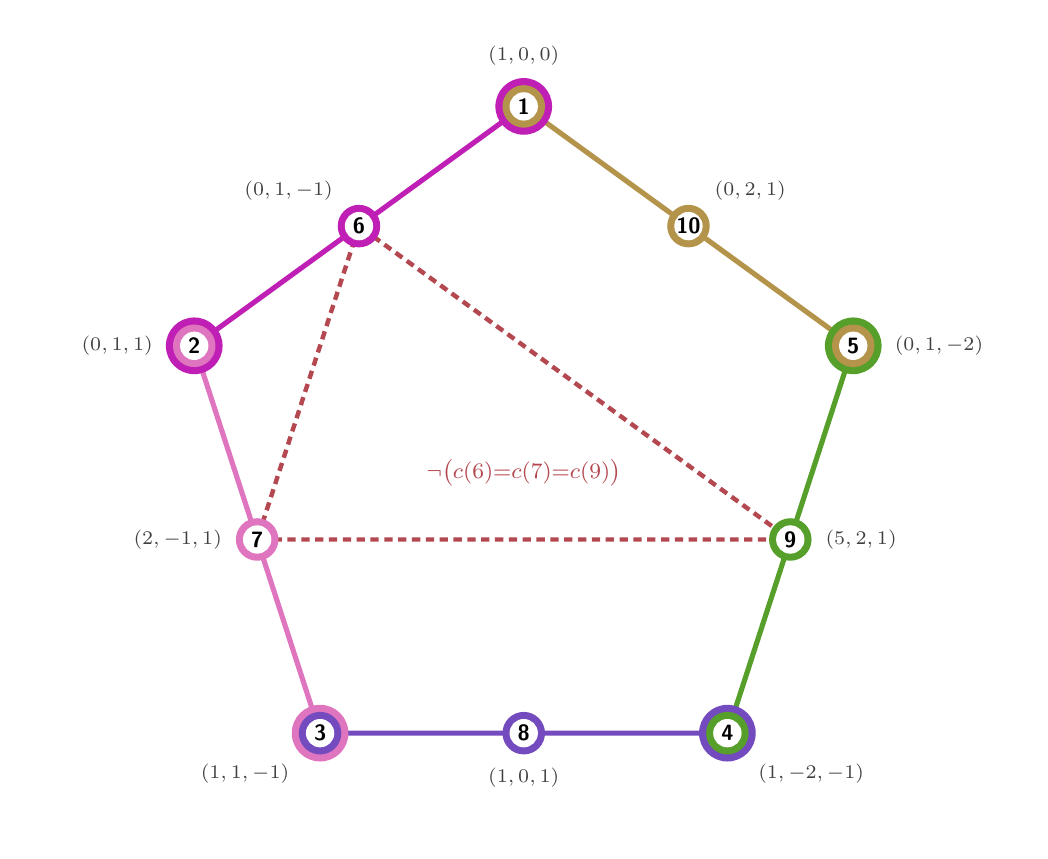
\begin{tikzpicture}[x=1cm,y=1cm]
    \def\R{4.4}%
    \foreach \v/\ang in {1/90,2/162,3/234,4/306,5/18}{%
      \coordinate (v\v) at (\ang:\R);
    }
    \coordinate (v6) at ($(v1)!.5!(v2)$);
    \coordinate (v7) at ($(v2)!.5!(v3)$);
    \coordinate (v8) at ($(v3)!.5!(v4)$);
    \coordinate (v9) at ($(v4)!.5!(v5)$);
    \coordinate (v10) at ($(v5)!.5!(v1)$);
    \draw[YOtrace,YOctx1]  (v1)--(v6)--(v2);
    \draw[YOtrace,YOctx9]  (v2)--(v7)--(v3);
    \draw[YOtrace,YOctx10] (v3)--(v8)--(v4);
    \draw[YOtrace,YOctx5]  (v4)--(v9)--(v5);
    \draw[YOtrace,YOctx8]  (v5)--(v10)--(v1);
    % Highlight 3-ary purely chromatic TIFS on {6,7,9}
    \draw[CSexcl,-] (v6) -- (v7) -- (v9) -- cycle;
    \node[CSnote,text=YOdiagonal] at (0,-0.25) {$\neg\bigl(c(6){=}c(7){=}c(9)\bigr)$};
    \YOvertex{1}{1/.36,8/.27}
    \YOvertex{2}{1/.36,9/.27}
    \YOvertex{3}{9/.36,10/.27}
    \YOvertex{4}{10/.36,5/.27}
    \YOvertex{5}{5/.36,8/.27}
    \YOvertex{6}{1/.27}
    \YOvertex{7}{9/.27}
    \YOvertex{8}{10/.27}
    \YOvertex{9}{5/.27}
    \YOvertex{10}{8/.27}
    % Integer FOR labels in R^3
    \node[CSvec,above=3pt] at ($(v1)+(0,.38)$) {$(1,0,0)$};
    \node[CSvec,left=3pt] at ($(v2)+(-.38,0)$) {$(0,1,1)$};
    \node[CSvec,below left=2pt] at ($(v3)+(-.28,-.28)$) {$(1,1,-1)$};
    \node[CSvec,below right=2pt] at ($(v4)+(.28,-.28)$) {$(1,-2,-1)$};
    \node[CSvec,right=3pt] at ($(v5)+(.38,0)$) {$(0,1,-2)$};
    \node[CSvec,above left=2pt] at ($(v6)+(-.22,.22)$) {$(0,1,-1)$};
    \node[CSvec,left=3pt] at ($(v7)+(-.30,0)$) {$(2,-1,1)$};
    \node[CSvec,below=3pt] at ($(v8)+(0,-.30)$) {$(1,0,1)$};
    \node[CSvec,right=3pt] at ($(v9)+(.30,0)$) {$(5,2,1)$};
    \node[CSvec,above right=2pt] at ($(v10)+(.22,.22)$) {$(0,2,1)$};
    \pgfresetboundingbox
    \path[use as bounding box] (-6.3,-4.8) rectangle (6.3,5.4);
  \end{tikzpicture}%
}

% (b) Completed Specker bug H_{13,7}: conventional regular hexagon with vertical crossbar (Fig. 1a)
\newcommand{\CSdrawSpeckerBug}{%
  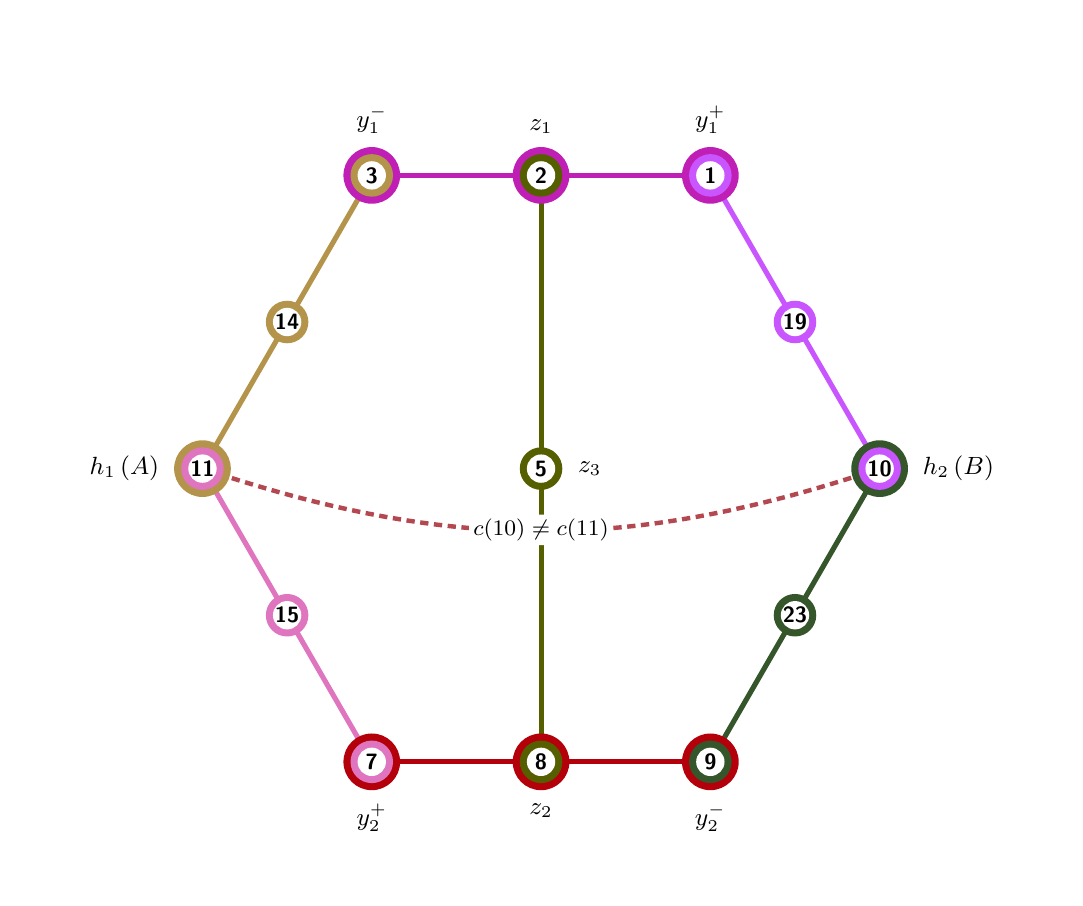
\begin{tikzpicture}[x=1cm,y=1cm]
    \def\R{4.3}%
    \coordinate (v10) at (  0:\R);
    \coordinate (v1)  at ( 60:\R);
    \coordinate (v3)  at (120:\R);
    \coordinate (v11) at (180:\R);
    \coordinate (v7)  at (240:\R);
    \coordinate (v9)  at (300:\R);
    \coordinate (v2)  at ($(v3)!.5!(v1)$);
    \coordinate (v8)  at ($(v7)!.5!(v9)$);
    \coordinate (v5)  at (0,0);
    \coordinate (v14) at ($(v11)!.5!(v3)$);
    \coordinate (v15) at ($(v11)!.5!(v7)$);
    \coordinate (v19) at ($(v1)!.5!(v10)$);
    \coordinate (v23) at ($(v9)!.5!(v10)$);
    % All 7 contexts are pure straight lines forming the conventional Specker bug hexagon:
    \draw[YOtrace,YOctx1]  (v3)--(v2)--(v1);
    \draw[YOtrace,YOctx2]  (v7)--(v8)--(v9);
    \draw[YOtrace,YOctx4]  (v2)--(v5)--(v8);
    \draw[YOtrace,YOctx8]  (v11)--(v14)--(v3);
    \draw[YOtrace,YOctx9]  (v11)--(v15)--(v7);
    \draw[YOtrace,YOctx12] (v1)--(v19)--(v10);
    \draw[YOtrace,YOctx11] (v9)--(v23)--(v10);
    \draw[CSexcl] (v11) to[bend right=18] node[CSnote,pos=.50] {$c(10)\ne c(11)$} (v10);
    \YOvertex{1}{1/.36,12/.27}
    \YOvertex{2}{1/.36,4/.27}
    \YOvertex{3}{1/.36,8/.27}
    \YOvertex{5}{4/.27}
    \YOvertex{7}{2/.36,9/.27}
    \YOvertex{8}{2/.36,4/.27}
    \YOvertex{9}{2/.36,11/.27}
    \YOvertex{10}{11/.36,12/.27}
    \YOvertex{11}{8/.36,9/.27}
    \YOvertex{14}{8/.27}
    \YOvertex{15}{9/.27}
    \YOvertex{19}{12/.27}
    \YOvertex{23}{11/.27}
    \node[YOlabel,left=4pt]  at ($(v11)+(-.36,0)$) {$h_1\,(A)$};
    \node[YOlabel,right=4pt] at ($(v10)+(.36,0)$)  {$h_2\,(B)$};
    \node[YOlabel,above=4pt] at ($(v3)+(0,.34)$)   {$y_1^-$};
    \node[YOlabel,above=4pt] at ($(v2)+(0,.34)$)   {$z_1$};
    \node[YOlabel,above=4pt] at ($(v1)+(0,.34)$)   {$y_1^+$};
    \node[YOlabel,below=4pt] at ($(v7)+(0,-.34)$)  {$y_2^+$};
    \node[YOlabel,below=4pt] at ($(v8)+(0,-.34)$)  {$z_2$};
    \node[YOlabel,below=4pt] at ($(v9)+(0,-.34)$)  {$y_2^-$};
    \node[YOlabel,right=4pt] at ($(v5)+(.28,0)$)   {$z_3$};
    \pgfresetboundingbox
    \path[use as bounding box] (-6.52,-5.2) rectangle (6.52,5.6);
  \end{tikzpicture}%
}

% (c) Purely Chromatic TIFS H_{16,9}^{TIFS} on the conventional Specker bug hexagon (all 9 contexts pure straight lines)
\newcommand{\CSdrawPureChromTIFS}{%
  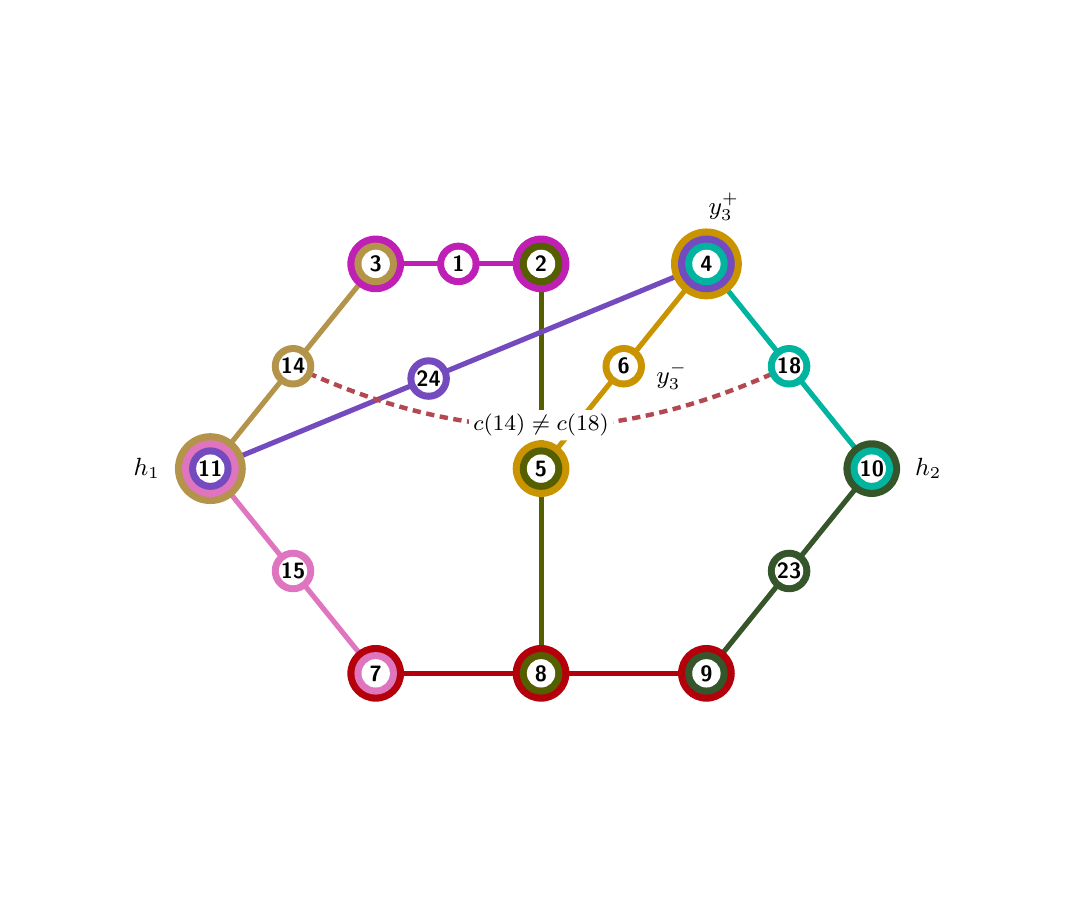
\begin{tikzpicture}[x=1cm,y=1cm]
    \coordinate (v11) at (-4.20, 0.00);
    \coordinate (v10) at ( 4.20, 0.00);
    \coordinate (v3)  at (-2.10, 2.60);
    \coordinate (v1)  at (-1.05, 2.60);
    \coordinate (v2)  at ( 0.00, 2.60);
    \coordinate (v4)  at ( 2.10, 2.60);
    \coordinate (v7)  at (-2.10,-2.60);
    \coordinate (v8)  at ( 0.00,-2.60);
    \coordinate (v9)  at ( 2.10,-2.60);
    \coordinate (v5)  at ( 0.00, 0.00);
    \coordinate (v6)  at ($(v5)!.5!(v4)$);
    \coordinate (v14) at ($(v11)!.5!(v3)$);
    \coordinate (v15) at ($(v11)!.5!(v7)$);
    \coordinate (v18) at ($(v10)!.5!(v4)$);
    \coordinate (v23) at ($(v9)!.5!(v10)$);
    \coordinate (v24) at ($(v11)!.44!(v4)$);
    % All 9 contexts are pure straight lines on the conventional Specker bug hexagon:
    \draw[YOtrace,YOctx1]  (v3)--(v1)--(v2);
    \draw[YOtrace,YOctx2]  (v7)--(v8)--(v9);
    \draw[YOtrace,YOctx3]  (v5)--(v6)--(v4);
    \draw[YOtrace,YOctx4]  (v2)--(v5)--(v8);
    \draw[YOtrace,YOctx8]  (v11)--(v14)--(v3);
    \draw[YOtrace,YOctx9]  (v11)--(v15)--(v7);
    \draw[YOtrace,YOctx11] (v9)--(v23)--(v10);
    \draw[YOtrace,YOctx13] (v10)--(v18)--(v4);
    \draw[YOtrace,YOctx10] (v11)--(v24)--(v4);
    \draw[CSexcl] (v14) to[bend right=24] node[CSnote,pos=.50] {$c(14)\ne c(18)$} (v18);
    \YOvertex{1}{1/.27}
    \YOvertex{2}{1/.36,4/.27}
    \YOvertex{3}{1/.36,8/.27}
    \YOvertex{4}{3/.45,10/.36,13/.27}
    \YOvertex{5}{3/.36,4/.27}
    \YOvertex{6}{3/.27}
    \YOvertex{7}{2/.36,9/.27}
    \YOvertex{8}{2/.36,4/.27}
    \YOvertex{9}{2/.36,11/.27}
    \YOvertex{10}{11/.36,13/.27}
    \YOvertex{11}{8/.45,9/.36,10/.27}
    \YOvertex{14}{8/.27}
    \YOvertex{15}{9/.27}
    \YOvertex{18}{13/.27}
    \YOvertex{23}{11/.27}
    \YOvertex{24}{10/.27}
    \node[YOlabel,left=4pt]  at ($(v11)+(-.45,0)$) {$h_1$};
    \node[YOlabel,right=4pt] at ($(v10)+(.36,0)$)  {$h_2$};
    \node[YOlabel,above=4pt] at ($(v4)+(.22,.36)$) {$y_3^+$};
    \node[YOlabel,right=3pt] at ($(v6)+(.26,-.12)$) {$y_3^-$};
    \pgfresetboundingbox
    \path[use as bounding box] (-6.52,-5.2) rectangle (6.52,5.6);
  \end{tikzpicture}%
}

% (d) Completed Kochen--Specker TITS H_{16,9}^{TITS}: all 9 contexts as pure straight lines on the Specker bug hexagon
\newcommand{\CSdrawCompletedKSTITS}{%
  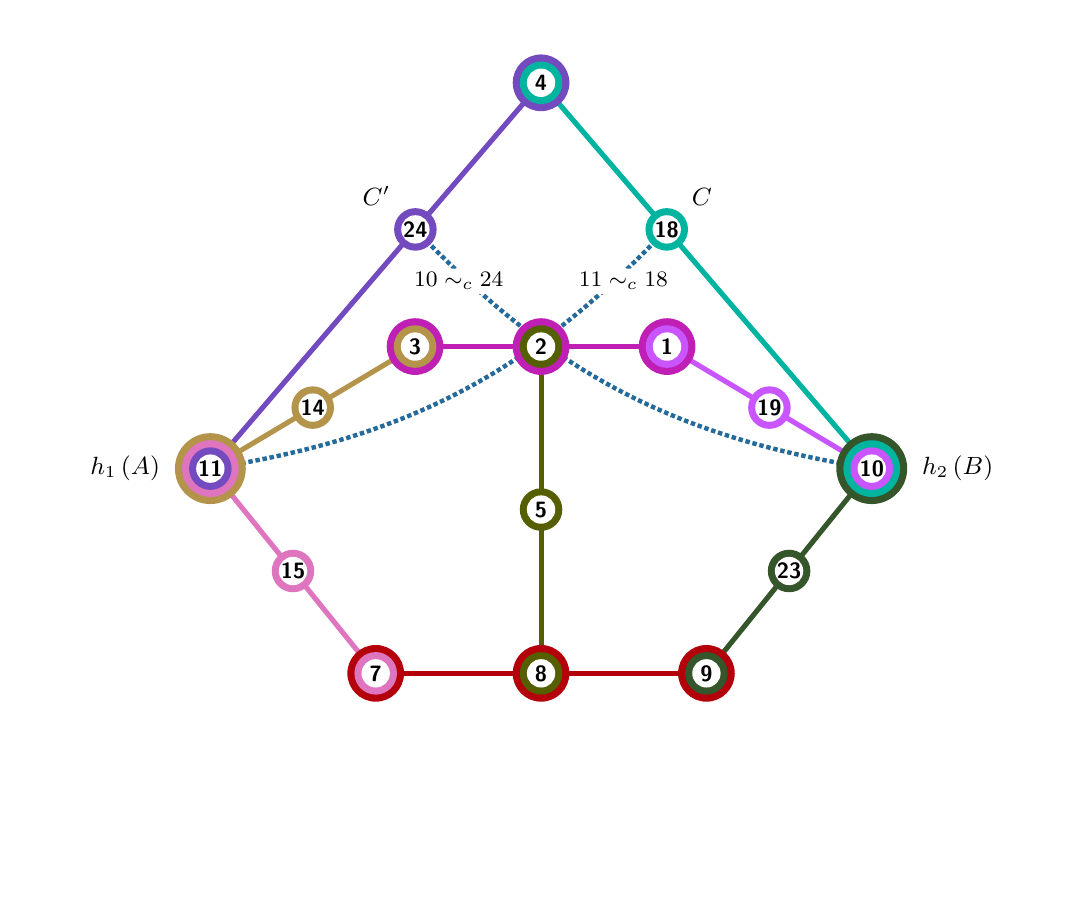
\begin{tikzpicture}[x=1cm,y=1cm]
    \coordinate (v11) at (-4.20, 0.00);
    \coordinate (v10) at ( 4.20, 0.00);
    \coordinate (v3)  at (-1.60, 1.55);
    \coordinate (v2)  at ( 0.00, 1.55);
    \coordinate (v1)  at ( 1.60, 1.55);
    \coordinate (v7)  at (-2.10,-2.60);
    \coordinate (v8)  at ( 0.00,-2.60);
    \coordinate (v9)  at ( 2.10,-2.60);
    \coordinate (v5)  at ( 0.00,-0.52);
    \coordinate (v14) at ($(v11)!.5!(v3)$);
    \coordinate (v15) at ($(v11)!.5!(v7)$);
    \coordinate (v19) at ($(v1)!.5!(v10)$);
    \coordinate (v23) at ($(v9)!.5!(v10)$);
    % Straight-line upper contexts {11,24,4} and {10,18,4} meeting at top apex v4=(0,4.90):
    \coordinate (v4)  at ( 0.00, 4.90);
    \coordinate (v24) at ($(v11)!.62!(v4)$);
    \coordinate (v18) at ($(v10)!.62!(v4)$);
    % All 9 contexts are pure straight lines:
    \draw[YOtrace,YOctx1]  (v3)--(v2)--(v1);
    \draw[YOtrace,YOctx2]  (v7)--(v8)--(v9);
    \draw[YOtrace,YOctx4]  (v2)--(v5)--(v8);
    \draw[YOtrace,YOctx8]  (v11)--(v14)--(v3);
    \draw[YOtrace,YOctx9]  (v11)--(v15)--(v7);
    \draw[YOtrace,YOctx12] (v1)--(v19)--(v10);
    \draw[YOtrace,YOctx11] (v9)--(v23)--(v10);
    \draw[YOtrace,YOctx10] (v11)--(v24)--(v4);
    \draw[YOtrace,YOctx13] (v10)--(v18)--(v4);
    \draw[CSident] (v11) to[bend right=18] (v18);
    \draw[CSident] (v10) to[bend left=18]  (v24);
    \node[CSnote,anchor=east] at (-0.42, 2.38) {$10\sim_c 24$};
    \node[CSnote,anchor=west] at ( 0.42, 2.38) {$11\sim_c 18$};
    \YOvertex{1}{1/.36,12/.27}
    \YOvertex{2}{1/.36,4/.27}
    \YOvertex{3}{1/.36,8/.27}
    \YOvertex{4}{10/.36,13/.27}
    \YOvertex{5}{4/.27}
    \YOvertex{7}{2/.36,9/.27}
    \YOvertex{8}{2/.36,4/.27}
    \YOvertex{9}{2/.36,11/.27}
    \YOvertex{10}{11/.45,13/.36,12/.27}
    \YOvertex{11}{8/.45,9/.36,10/.27}
    \YOvertex{14}{8/.27}
    \YOvertex{15}{9/.27}
    \YOvertex{18}{13/.27}
    \YOvertex{19}{12/.27}
    \YOvertex{23}{11/.27}
    \YOvertex{24}{10/.27}
    \node[YOlabel,left=4pt]       at ($(v11)+(-.45,0)$) {$h_1\,(A)$};
    \node[YOlabel,right=4pt]      at ($(v10)+(.45,0)$)  {$h_2\,(B)$};
    \node[YOlabel,above left=2pt]  at ($(v24)+(-.20,.18)$) {$C'$};
    \node[YOlabel,above right=2pt] at ($(v18)+(.20,.18)$)  {$C$};
    \pgfresetboundingbox
    \path[use as bounding box] (-6.52,-5.2) rectangle (6.52,5.6);
  \end{tikzpicture}%
}

% (e) Two-way purely chromatic TITS H_{19,11}^{TITS}: all 11 contexts as pure straight lines on the Specker bug hexagon
\newcommand{\CSdrawPureChromTITS}{%
  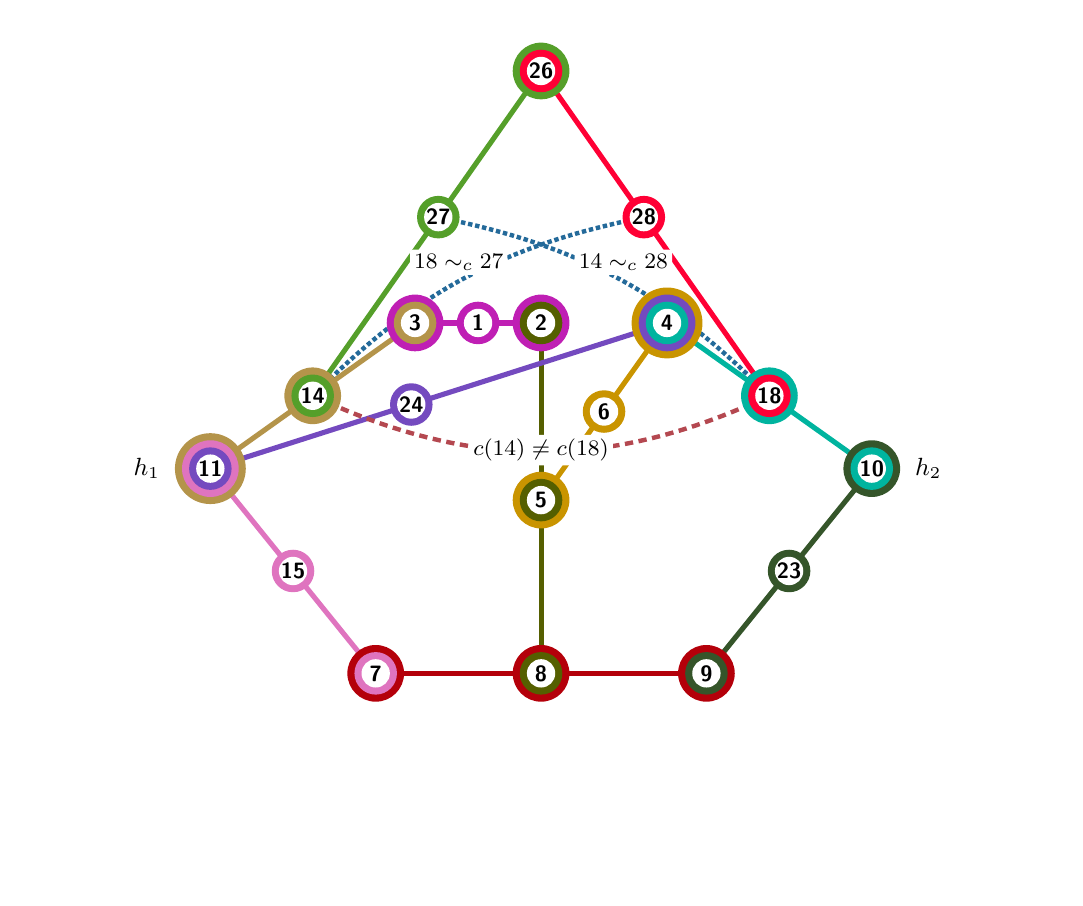
\begin{tikzpicture}[x=1cm,y=1cm]
    \coordinate (v11) at (-4.20, 0.00);
    \coordinate (v10) at ( 4.20, 0.00);
    \coordinate (v3)  at (-1.60, 1.85);
    \coordinate (v1)  at (-0.80, 1.85);
    \coordinate (v2)  at ( 0.00, 1.85);
    \coordinate (v4)  at ( 1.60, 1.85);
    \coordinate (v7)  at (-2.10,-2.60);
    \coordinate (v8)  at ( 0.00,-2.60);
    \coordinate (v9)  at ( 2.10,-2.60);
    \coordinate (v5)  at ( 0.00,-0.40);
    \coordinate (v6)  at ($(v5)!.5!(v4)$);
    \coordinate (v14) at ($(v11)!.5!(v3)$);
    \coordinate (v15) at ($(v11)!.5!(v7)$);
    \coordinate (v18) at ($(v10)!.5!(v4)$);
    \coordinate (v23) at ($(v9)!.5!(v10)$);
    \coordinate (v24) at ($(v11)!.44!(v4)$);
    % Symmetric upper straight-line roof contexts {14,27,26} and {18,28,26} meeting at v26=(0,5.05)
    \coordinate (v26) at ( 0.00, 5.05);
    \coordinate (v27) at ($(v14)!.55!(v26)$);
    \coordinate (v28) at ($(v18)!.55!(v26)$);
    % All 11 contexts are pure straight lines:
    \draw[YOtrace,YOctx1]  (v3)--(v1)--(v2);
    \draw[YOtrace,YOctx2]  (v7)--(v8)--(v9);
    \draw[YOtrace,YOctx3]  (v5)--(v6)--(v4);
    \draw[YOtrace,YOctx4]  (v2)--(v5)--(v8);
    \draw[YOtrace,YOctx8]  (v11)--(v14)--(v3);
    \draw[YOtrace,YOctx9]  (v11)--(v15)--(v7);
    \draw[YOtrace,YOctx11] (v9)--(v23)--(v10);
    \draw[YOtrace,YOctx13] (v10)--(v18)--(v4);
    \draw[YOtrace,YOctx10] (v11)--(v24)--(v4);
    \draw[YOtrace,YOctx5]  (v14)--(v27)--(v26);
    \draw[YOtrace,YOctx16] (v18)--(v28)--(v26);
    \draw[CSexcl]  (v14) to[bend right=24] node[CSnote,pos=.50] {$c(14)\ne c(18)$} (v18);
    \draw[CSident] (v14) to[bend left=16]  (v28);
    \draw[CSident] (v18) to[bend right=16] (v27);
    \node[CSnote,anchor=east] at (-0.42, 2.62) {$18\sim_c 27$};
    \node[CSnote,anchor=west] at ( 0.42, 2.62) {$14\sim_c 28$};
    \YOvertex{1}{1/.27}
    \YOvertex{2}{1/.36,4/.27}
    \YOvertex{3}{1/.36,8/.27}
    \YOvertex{4}{3/.45,10/.36,13/.27}
    \YOvertex{5}{3/.36,4/.27}
    \YOvertex{6}{3/.27}
    \YOvertex{7}{2/.36,9/.27}
    \YOvertex{8}{2/.36,4/.27}
    \YOvertex{9}{2/.36,11/.27}
    \YOvertex{10}{11/.36,13/.27}
    \YOvertex{11}{8/.45,9/.36,10/.27}
    \YOvertex{14}{8/.36,5/.27}
    \YOvertex{15}{9/.27}
    \YOvertex{18}{13/.36,16/.27}
    \YOvertex{23}{11/.27}
    \YOvertex{24}{10/.27}
    \YOvertex{26}{5/.36,16/.27}
    \YOvertex{27}{5/.27}
    \YOvertex{28}{16/.27}
    \node[YOlabel,left=4pt]  at ($(v11)+(-.45,0)$) {$h_1$};
    \node[YOlabel,right=4pt] at ($(v10)+(.36,0)$)  {$h_2$};
    \pgfresetboundingbox
    \path[use as bounding box] (-6.52,-5.2) rectangle (6.52,5.6);
  \end{tikzpicture}%
}

% (f) Three-sector Yu-Oh H_{21,13}: ALL 13 contexts drawn as pure straight lines on the conventional Specker bug hexagon
\newcommand{\CSdrawHtwentyoneTITS}{%
  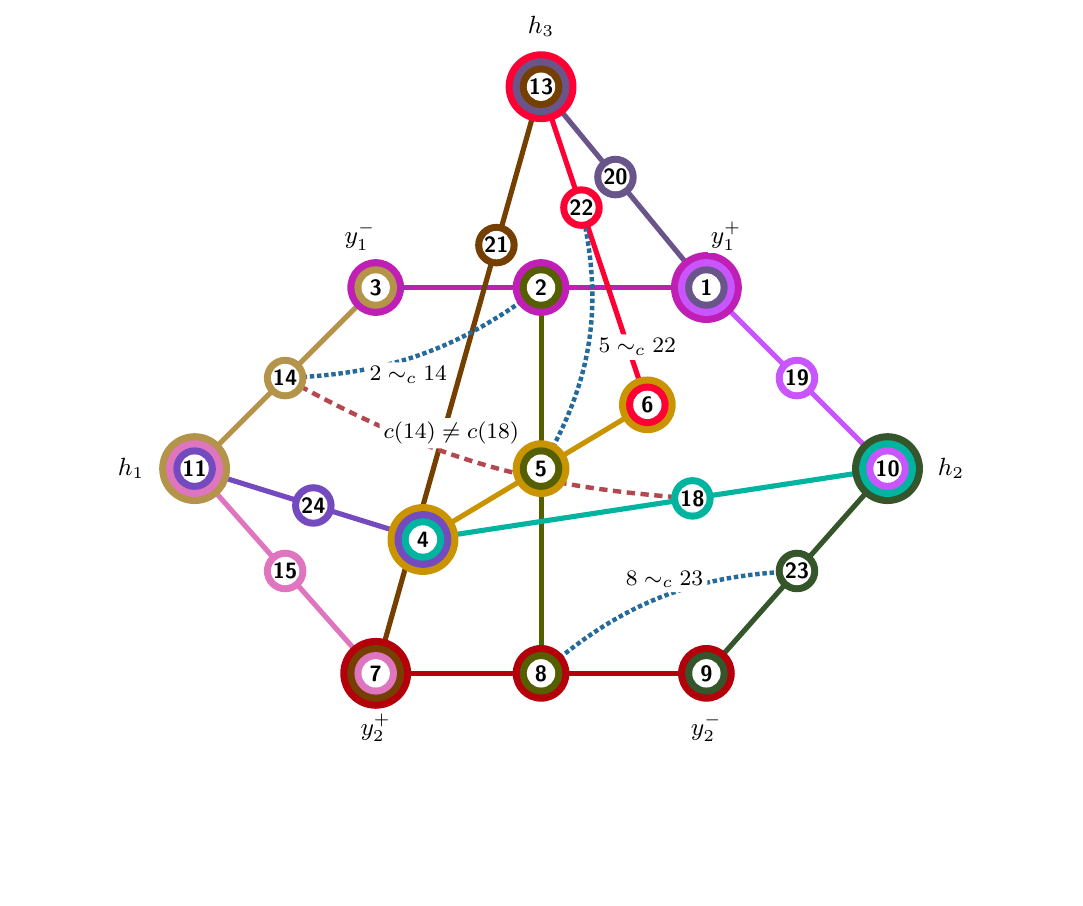
\begin{tikzpicture}[x=1cm,y=1cm]
    % Conventional Specker bug hexagon (7 straight lines):
    \coordinate (v11) at (-4.40, 0.00);
    \coordinate (v10) at ( 4.40, 0.00);
    \coordinate (v3)  at (-2.10, 2.30);
    \coordinate (v2)  at ( 0.00, 2.30);
    \coordinate (v1)  at ( 2.10, 2.30);
    \coordinate (v7)  at (-2.10,-2.60);
    \coordinate (v8)  at ( 0.00,-2.60);
    \coordinate (v9)  at ( 2.10,-2.60);
    \coordinate (v5)  at ( 0.00, 0.00);
    \coordinate (v14) at ($(v11)!.5!(v3)$);
    \coordinate (v15) at ($(v11)!.5!(v7)$);
    \coordinate (v19) at ($(v1)!.5!(v10)$);
    \coordinate (v23) at ($(v9)!.5!(v10)$);
    % Context {4,5,6} as a straight line through v5=(0,0), plus straight lines {11,24,4} and {10,18,4}:
    \coordinate (v4)  at (-1.50,-0.90);
    \coordinate (v6)  at ( 1.35, 0.81);
    \coordinate (v24) at ($(v11)!.52!(v4)$);
    \coordinate (v18) at ($(v10)!.42!(v4)$);
    % Third hub v13=(0,4.85) at the top apex with 3 straight lines {13,20,1}, {13,22,6}, {13,21,7}:
    \coordinate (v13) at ( 0.00, 4.85);
    \coordinate (v20) at ($(v13)!.45!(v1)$);
    \coordinate (v22) at ($(v13)!.38!(v6)$);
    \coordinate (v21) at ($(v13)!.27!(v7)$);
    % All 13 contexts are pure straight lines:
    \draw[YOtrace,YOctx1]  (v3)--(v2)--(v1);
    \draw[YOtrace,YOctx2]  (v7)--(v8)--(v9);
    \draw[YOtrace,YOctx3]  (v4)--(v5)--(v6);
    \draw[YOtrace,YOctx4]  (v2)--(v5)--(v8);
    \draw[YOtrace,YOctx8]  (v11)--(v14)--(v3);
    \draw[YOtrace,YOctx9]  (v11)--(v15)--(v7);
    \draw[YOtrace,YOctx11] (v9)--(v23)--(v10);
    \draw[YOtrace,YOctx12] (v1)--(v19)--(v10);
    \draw[YOtrace,YOctx10] (v11)--(v24)--(v4);
    \draw[YOtrace,YOctx13] (v10)--(v18)--(v4);
    \draw[YOtrace,YOctx16] (v6)--(v22)--(v13);
    \draw[YOtrace,YOctx14] (v13)--(v20)--(v1);
    \draw[YOtrace,YOctx15] (v13)--(v21)--(v7);
    % Highlight two-way purely chromatic TITSs 2~14, 5~22, 8~23 and purely chromatic TIFS c(14)!=c(18)
    \draw[CSident] (v2) to[bend left=16]  node[CSnote,pos=.55,below=1pt] {$2\sim_c 14$} (v14);
    \draw[CSident] (v8) to[bend left=18]  node[CSnote,pos=.52,above=1pt] {$8\sim_c 23$} (v23);
    \draw[CSident] (v5) to[bend right=20] node[CSnote,pos=.48,right=2pt] {$5\sim_c 22$} (v22);
    \draw[CSexcl]  (v14) to[bend right=12] node[CSnote,pos=.42,above=1pt] {$c(14)\ne c(18)$} (v18);
    \CSHtwentyonevertices
    \node[YOlabel,left=4pt]  at ($(v11)+(-.45,0)$) {$h_1$};
    \node[YOlabel,right=4pt] at ($(v10)+(.45,0)$)  {$h_2$};
    \node[YOlabel,above=4pt] at ($(v13)+(0,.45)$)  {$h_3$};
    \node[YOlabel,above=3pt] at ($(v3)+(-.20,.32)$) {$y_1^-$};
    \node[YOlabel,above=3pt] at ($(v1)+(.25,.32)$)  {$y_1^+$};
    \node[YOlabel,below=3pt] at ($(v7)+(0,-.36)$)   {$y_2^+$};
    \node[YOlabel,below=3pt] at ($(v9)+(0,-.36)$)   {$y_2^-$};
    \pgfresetboundingbox
    \path[use as bounding box] (-6.52,-5.2) rectangle (6.52,5.6);
  \end{tikzpicture}%
}
% END INLINED FILE: figures/chromatic-gadgets-3d.tex

% BEGIN INLINED FILE: figures/chromatic-gadgets-4d.tex
% Macros copied verbatim from chromatic-tifs-tits-d4-standalone.tex.
\tikzset{
  CSexcl/.style={draw=YOdiagonal,line width=1.6pt,densely dashed,{Latex[length=2.4mm]}-{Latex[length=2.4mm]}},
  CSident/.style={draw=YOtriad,line width=1.6pt,densely dotted,{Latex[length=2.4mm]}-{Latex[length=2.4mm]}},
  CSnote/.style={font=\sffamily\footnotesize,fill=white,inner sep=1.5pt,rounded corners=1pt},
  CSvec/.style={font=\scriptsize,text=black!75,inner sep=1pt},
}

% Helper macro for continuous solid 4-vertex hyperedges extending smoothly
% (C^1-tangentially) past an endpoint of a 3D straight-line triad into (v0):
\providecommand{\CSsolidapex}[7]{%
  \draw[YOtrace,YOctx#1] (#2)--(#3)--(#4)
    -- ($(#4)!-#5!(#2)$)
    .. controls ($(#4)!-#6!(#2)$) and #7 .. (v0);%
}

% (a) 5-Wheel W_5^{(4)}: 11 rays, 5 contexts in R^4; each context is an open circular arc starting at v0 and ending at v_{i+1}
\newcommand{\CSdrawWfiveFour}{%
  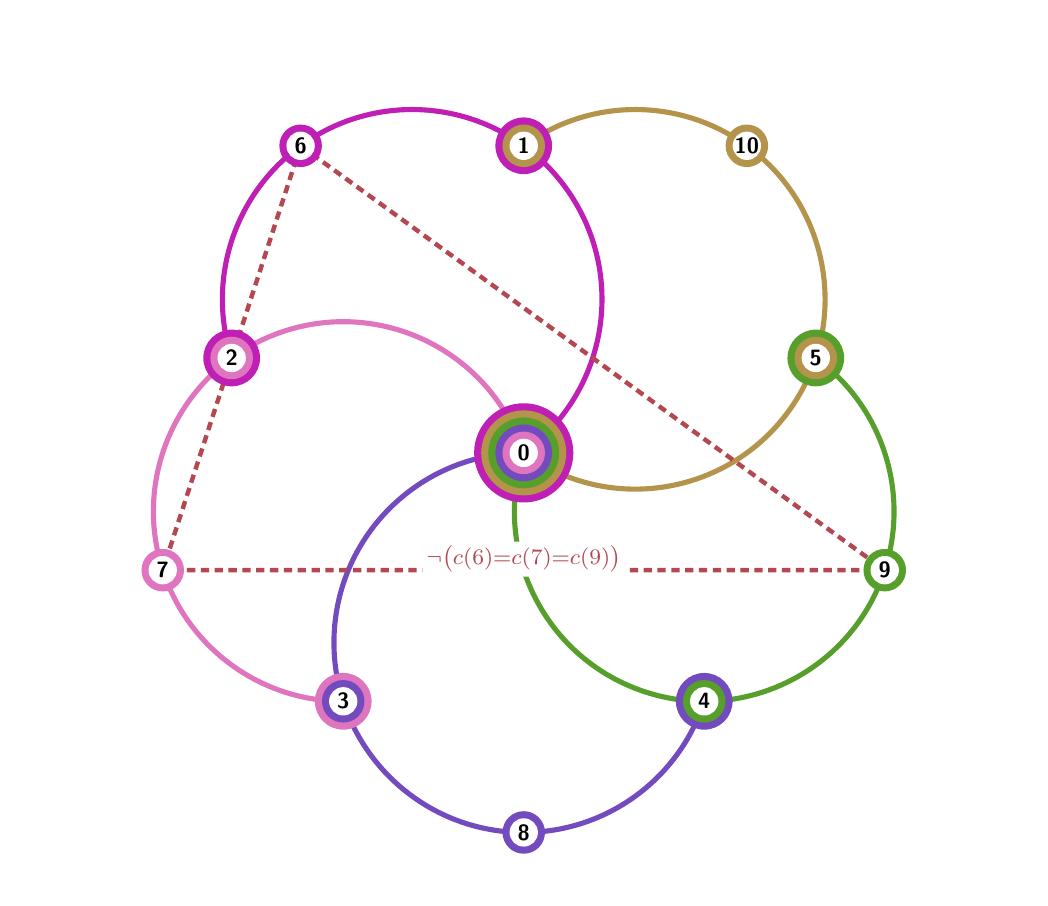
\begin{tikzpicture}[x=1cm,y=1cm]
    \def\R{3.9}%
    \pgfmathsetmacro{\rc}{\R/(2*cos(36))}%
    \coordinate (v0) at (0,0);
    \foreach \v/\ang in {1/90,2/162,3/234,4/306,5/18}{%
      \coordinate (v\v) at (\ang:\R);
    }
    % Each degree-1 vertex lies at the outer crest (2*rc) of the unique circle through (v0, v_i, v_{i+1})
    \foreach \v/\ang in {6/126,7/198,8/270,9/342,10/54}{%
      \coordinate (v\v) at (\ang:{2*\rc});
    }
    % 5 4-uniform contexts drawn as open circular arcs starting at v0 and ending at v_{i+1}:
    \draw[YOtrace,YOctx1]  (0,0) arc (126-180:126+72:\rc);
    \draw[YOtrace,YOctx9]  (0,0) arc (198-180:198+72:\rc);
    \draw[YOtrace,YOctx10] (0,0) arc (270-180:270+72:\rc);
    \draw[YOtrace,YOctx5]  (0,0) arc (342-180:342+72:\rc);
    \draw[YOtrace,YOctx8]  (0,0) arc ( 54-180: 54+72:\rc);
    % Highlight 3-ary purely chromatic TIFS on {6,7,9}
    \draw[CSexcl,-] (v6) -- (v7) -- (v9) -- cycle;
    \node[CSnote,text=YOdiagonal] at (0,-1.35) {$\neg\bigl(c(6){=}c(7){=}c(9)\bigr)$};
    \YOvertex{0}{1/.63,8/.54,5/.45,10/.36,9/.27}
    \YOvertex{1}{1/.36,8/.27}
    \YOvertex{2}{1/.36,9/.27}
    \YOvertex{3}{9/.36,10/.27}
    \YOvertex{4}{10/.36,5/.27}
    \YOvertex{5}{5/.36,8/.27}
    \YOvertex{6}{1/.27}
    \YOvertex{7}{9/.27}
    \YOvertex{8}{10/.27}
    \YOvertex{9}{5/.27}
    \YOvertex{10}{8/.27}
    \pgfresetboundingbox
    \path[use as bounding box] (-6.3,-5.4) rectangle (6.3,5.4);
  \end{tikzpicture}%
}

% (b) Strictly Linear 5-Wheel W_5^{(4,lin)}: 16 rays, 6 contexts in R^4; ALL 6 contexts drawn as pure straight lines
\newcommand{\CSdrawWfiveLinFour}{%
  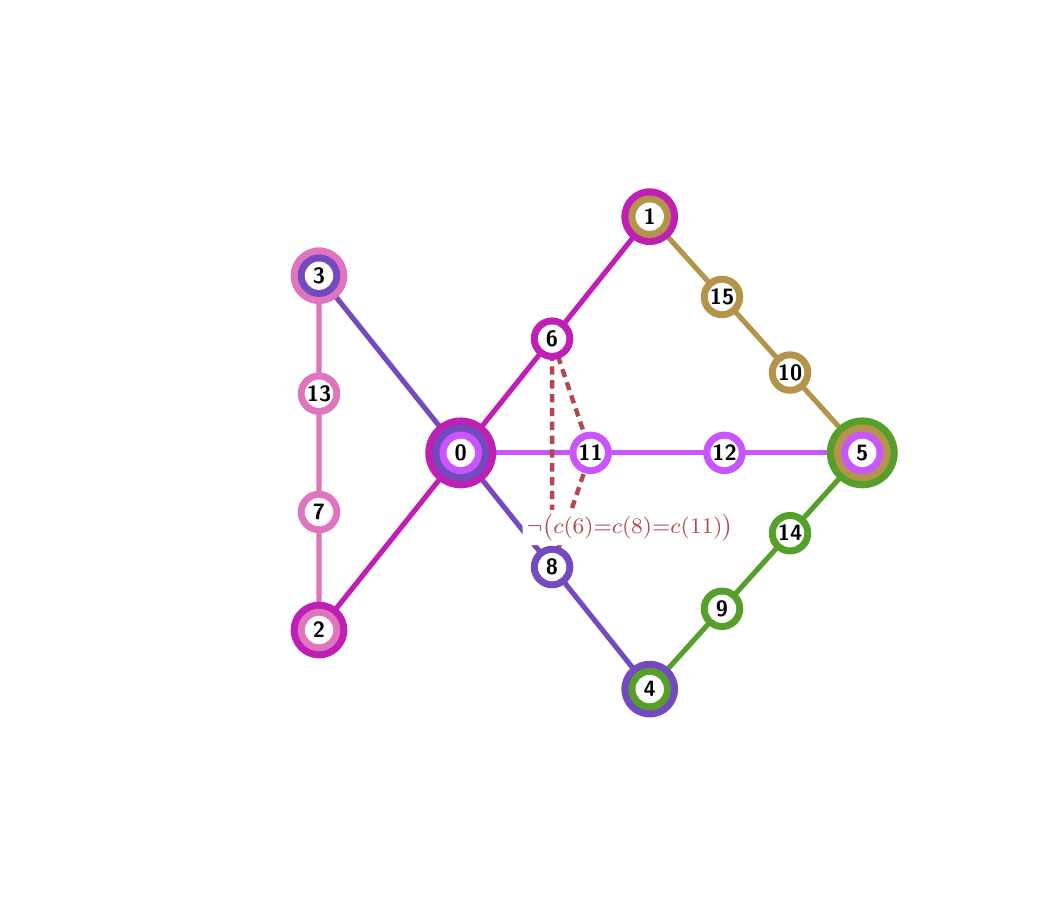
\begin{tikzpicture}[x=1cm,y=1cm]
    % Symmetric straight-line X-plus-pentagon layout:
    % C1={2,0,6,1} and C3={3,0,8,4} are the two straight diagonals crossing at v0=(-0.80,0);
    % C6={0,11,12,5} is the horizontal centerline; C2={2,7,13,3}, C4={4,9,14,5}, C5={5,10,15,1} are the outer sides.
    \coordinate (v0)  at (-0.80, 0.00);
    \coordinate (v2)  at (-2.60,-2.25);
    \coordinate (v6)  at ( 0.36, 1.45);
    \coordinate (v1)  at ( 1.60, 3.00);
    \coordinate (v3)  at (-2.60, 2.25);
    \coordinate (v8)  at ( 0.36,-1.45);
    \coordinate (v4)  at ( 1.60,-3.00);
    \coordinate (v11) at ( 0.85, 0.00);
    \coordinate (v12) at ( 2.55, 0.00);
    \coordinate (v5)  at ( 4.30, 0.00);
    \coordinate (v7)  at ($(v2)!.333!(v3)$);
    \coordinate (v13) at ($(v2)!.667!(v3)$);
    \coordinate (v9)  at ($(v4)!.34!(v5)$);
    \coordinate (v14) at ($(v4)!.66!(v5)$);
    \coordinate (v10) at ($(v5)!.34!(v1)$);
    \coordinate (v15) at ($(v5)!.66!(v1)$);
    % All 6 contexts are pure straight lines broken at sharp angles:
    \draw[YOtrace,YOctx1]  (v2)--(v0)--(v6)--(v1);
    \draw[YOtrace,YOctx9]  (v2)--(v7)--(v13)--(v3);
    \draw[YOtrace,YOctx10] (v3)--(v0)--(v8)--(v4);
    \draw[YOtrace,YOctx5]  (v4)--(v9)--(v14)--(v5);
    \draw[YOtrace,YOctx8]  (v5)--(v10)--(v15)--(v1);
    \draw[YOtrace,YOctx12] (v0)--(v11)--(v12)--(v5);
    % Highlight 3-ary purely chromatic TIFS on {6,8,11}
    \draw[CSexcl,-] (v6) -- (v8) -- (v11) -- cycle;
    \node[CSnote,text=YOdiagonal] at (1.35,-0.95) {$\neg\bigl(c(6){=}c(8){=}c(11)\bigr)$};
    \YOvertex{0}{1/.45,10/.36,12/.27}
    \YOvertex{1}{1/.36,8/.27}
    \YOvertex{2}{1/.36,9/.27}
    \YOvertex{3}{9/.36,10/.27}
    \YOvertex{4}{10/.36,5/.27}
    \YOvertex{5}{5/.45,8/.36,12/.27}
    \YOvertex{6}{1/.27}
    \YOvertex{7}{9/.27}
    \YOvertex{13}{9/.27}
    \YOvertex{8}{10/.27}
    \YOvertex{9}{5/.27}
    \YOvertex{14}{5/.27}
    \YOvertex{10}{8/.27}
    \YOvertex{15}{8/.27}
    \YOvertex{11}{12/.27}
    \YOvertex{12}{12/.27}
    \pgfresetboundingbox
    \path[use as bounding box] (-6.3,-5.4) rectangle (6.3,5.4);
  \end{tikzpicture}%
}

% (c) Coned Specker--Hardy Bug H_{14,7}^{(4)}: canonical Specker bug with solid C^1 tangent extensions to exterior v0
\newcommand{\CSdrawSpeckerHardyFour}{%
  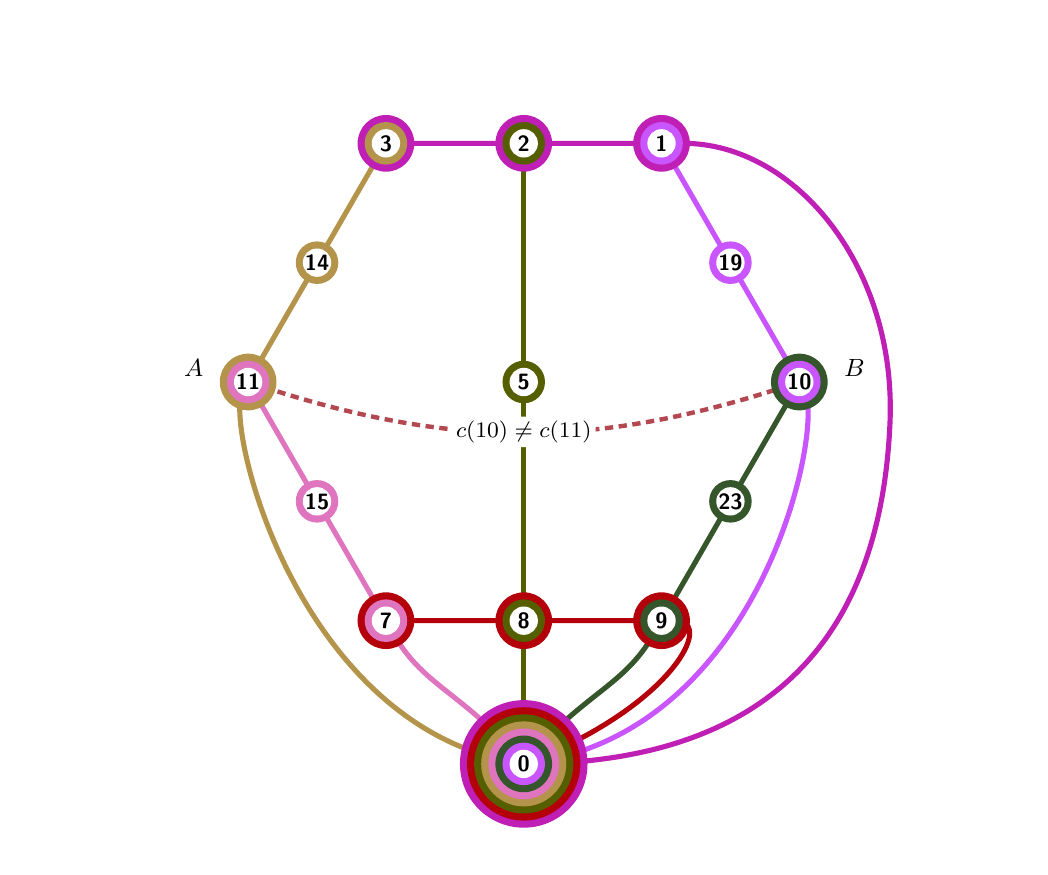
\begin{tikzpicture}[x=1cm,y=1cm]
    \def\R{3.50}%
    \coordinate (v10) at (  0:\R);
    \coordinate (v1)  at ( 60:\R);
    \coordinate (v3)  at (120:\R);
    \coordinate (v11) at (180:\R);
    \coordinate (v7)  at (240:\R);
    \coordinate (v9)  at (300:\R);
    \coordinate (v2)  at ($(v3)!.5!(v1)$);
    \coordinate (v8)  at ($(v7)!.5!(v9)$);
    \coordinate (v5)  at (0, 0.00);
    \coordinate (v0)  at (0,-4.85);
    \coordinate (v14) at ($(v11)!.5!(v3)$);
    \coordinate (v15) at ($(v11)!.5!(v7)$);
    \coordinate (v19) at ($(v1)!.5!(v10)$);
    \coordinate (v23) at ($(v9)!.5!(v10)$);

    % All 7 four-vertex contexts drawn as strictly nested, non-crossing SOLID hyperedges:
    % 1. Center vertical crossbar {2,5,8,0}: pure straight line
    \draw[YOtrace,YOctx4] (v2)--(v5)--(v8)--(v0);
    % 2. Left Lane 1 (inner): lower-left leg {11,15,7,0} extending down-right past v7
    \CSsolidapex{9}{v11}{v15}{v7}{0.06}{0.28}{(-0.75,-3.95)}
    % 3. Left Lane 2 (outer): upper-left leg {3,14,11,0} extending briefly past v11, hugging outside v15,v7
    \CSsolidapex{8}{v3}{v14}{v11}{0.04}{0.18}{(-2.85,-4.45)}
    % 4. Right Lane 1 (innermost): lower-right leg {10,23,9,0} extending down-left past v9
    \CSsolidapex{11}{v10}{v23}{v9}{0.06}{0.28}{( 0.75,-3.95)}
    % 5. Right Lane 2 (middle-inner): bottom bar {7,8,9,0} extending briefly right past v9
    \CSsolidapex{2}{v7}{v8}{v9}{0.05}{0.20}{( 1.85,-4.15)}
    % 6. Right Lane 3 (middle-outer): upper-right leg {1,19,10,0} extending briefly past v10, hugging outside v23,v9
    \CSsolidapex{12}{v1}{v19}{v10}{0.04}{0.18}{( 3.05,-4.50)}
    % 7. Right Lane 4 (outermost): top bar {3,2,1,0} sweeping wide outside v10 to v0
    \draw[YOtrace,YOctx1] (v3)--(v2)--(v1)
      -- ($(v1)!-0.08!(v3)$)
      .. controls ( 3.45, 3.03) and ( 4.75, 1.45) .. ( 4.65,-0.55)
      .. controls ( 4.55,-2.65) and ( 3.65,-4.85) .. (v0);

    \draw[CSexcl] (v11) to[bend right=18] node[CSnote,pos=.50] {$c(10)\ne c(11)$} (v10);

    \YOvertex{0}{1/.81,2/.72,4/.63,8/.54,9/.45,11/.36,12/.27}
    \YOvertex{1}{1/.36,12/.27}
    \YOvertex{2}{1/.36,4/.27}
    \YOvertex{3}{1/.36,8/.27}
    \YOvertex{5}{4/.27}
    \YOvertex{7}{2/.36,9/.27}
    \YOvertex{8}{2/.36,4/.27}
    \YOvertex{9}{2/.36,11/.27}
    \YOvertex{10}{11/.36,12/.27}
    \YOvertex{11}{8/.36,9/.27}
    \YOvertex{14}{8/.27}
    \YOvertex{15}{9/.27}
    \YOvertex{19}{12/.27}
    \YOvertex{23}{11/.27}
    \node[YOlabel,left=4pt]  at ($(v11)+(-.38,0.18)$) {$A$};
    \node[YOlabel,right=4pt] at ($(v10)+(.38,0.18)$)  {$B$};
    \pgfresetboundingbox
    \path[use as bounding box] (-6.3,-5.9) rectangle (6.3,4.5);
  \end{tikzpicture}%
}

% (d) Strictly Linear 7-Context Quaternion TIFS H_{18,7}^{(4,lin)}: 18 rays, 7 pure straight-line contexts in R^4
\newcommand{\CSdrawStrictLinTIFSFour}{%
  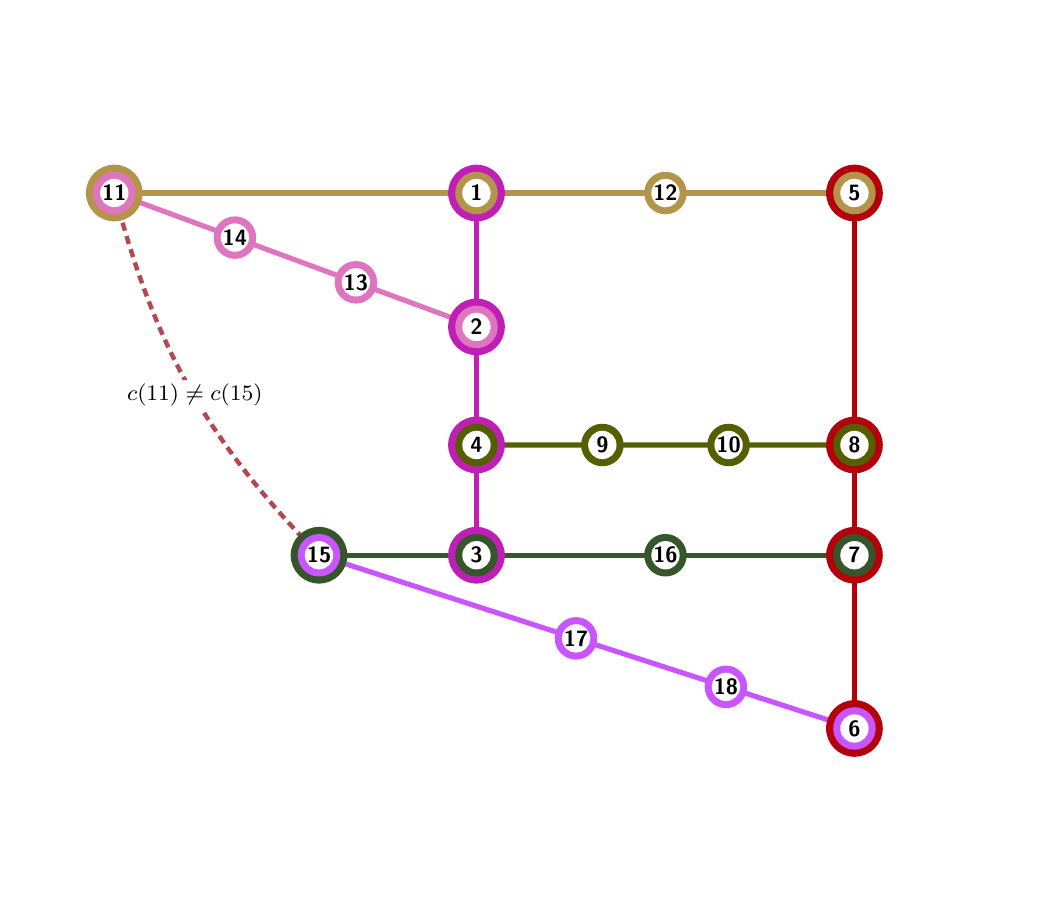
\begin{tikzpicture}[x=1cm,y=1cm]
    % C1={1,2,4,3}: vertical straight line at x=-0.6; C2={5,8,7,6}: vertical straight line at x=4.2
    \coordinate (v1) at (-0.60, 3.30);
    \coordinate (v2) at (-0.60, 1.60);
    \coordinate (v4) at (-0.60, 0.10);
    \coordinate (v3) at (-0.60,-1.30);
    \coordinate (v5) at ( 4.20, 3.30);
    \coordinate (v8) at ( 4.20, 0.10);
    \coordinate (v7) at ( 4.20,-1.30);
    \coordinate (v6) at ( 4.20,-3.50);
    % C3={4,9,10,8}: horizontal straight line at y=0.10
    \coordinate (v9)  at ($(v4)!.333!(v8)$);
    \coordinate (v10) at ($(v4)!.667!(v8)$);
    % C4={11,1,12,5}: horizontal straight line at y=3.30; C5={11,14,13,2}: diagonal straight line
    \coordinate (v11) at (-5.20, 3.30);
    \coordinate (v12) at ($(v1)!.50!(v5)$);
    \coordinate (v14) at ($(v11)!.333!(v2)$);
    \coordinate (v13) at ($(v11)!.667!(v2)$);
    % C6={15,3,16,7}: horizontal straight line at y=-1.30; C7={15,17,18,6}: diagonal straight line
    \coordinate (v15) at (-2.60,-1.30);
    \coordinate (v16) at ($(v3)!.50!(v7)$);
    \coordinate (v17) at ($(v15)!.48!(v6)$);
    \coordinate (v18) at ($(v15)!.76!(v6)$);
    % Draw all 7 4-uniform contexts as pure straight lines (zero crossings!):
    \draw[YOtrace,YOctx1]  (v1)--(v2)--(v4)--(v3);
    \draw[YOtrace,YOctx2]  (v5)--(v8)--(v7)--(v6);
    \draw[YOtrace,YOctx4]  (v4)--(v9)--(v10)--(v8);
    \draw[YOtrace,YOctx8]  (v11)--(v1)--(v12)--(v5);
    \draw[YOtrace,YOctx9]  (v11)--(v14)--(v13)--(v2);
    \draw[YOtrace,YOctx11] (v15)--(v3)--(v16)--(v7);
    \draw[YOtrace,YOctx12] (v15)--(v17)--(v18)--(v6);
    % Highlight binary TIFS c(11)!=c(15)
    \draw[CSexcl] (v11) to[bend right=14] node[CSnote,pos=.52] {$c(11)\ne c(15)$} (v15);
    \YOvertex{1}{1/.36,8/.27}
    \YOvertex{2}{1/.36,9/.27}
    \YOvertex{3}{1/.36,11/.27}
    \YOvertex{4}{1/.36,4/.27}
    \YOvertex{5}{2/.36,8/.27}
    \YOvertex{6}{2/.36,12/.27}
    \YOvertex{7}{2/.36,11/.27}
    \YOvertex{8}{2/.36,4/.27}
    \YOvertex{9}{4/.27}
    \YOvertex{10}{4/.27}
    \YOvertex{11}{8/.36,9/.27}
    \YOvertex{12}{8/.27}
    \YOvertex{13}{9/.27}
    \YOvertex{14}{9/.27}
    \YOvertex{15}{11/.36,12/.27}
    \YOvertex{16}{11/.27}
    \YOvertex{17}{12/.27}
    \YOvertex{18}{12/.27}
    \pgfresetboundingbox
    \path[use as bounding box] (-6.3,-5.4) rectangle (6.3,5.4);
  \end{tikzpicture}%
}

% (e) Purely Chromatic Binary TIFS H_{17,9}^{(4,TIFS)}: canonical D_{16,9} with solid C^1 tangent extensions to exterior v0
\newcommand{\CSdrawPureChromTIFSFour}{%
  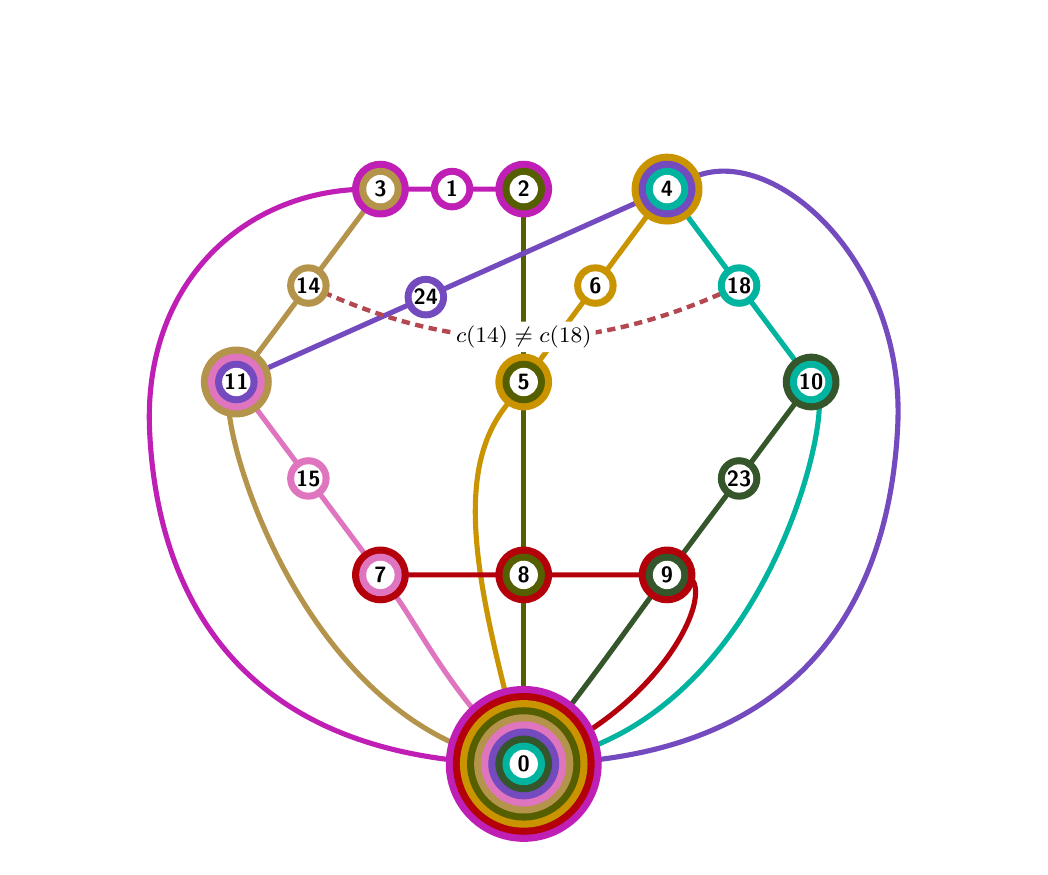
\begin{tikzpicture}[x=1cm,y=1cm]
    \coordinate (v11) at (-3.65, 0.00);
    \coordinate (v10) at ( 3.65, 0.00);
    \coordinate (v3)  at (-1.82, 2.45);
    \coordinate (v1)  at (-0.91, 2.45);
    \coordinate (v2)  at ( 0.00, 2.45);
    \coordinate (v4)  at ( 1.82, 2.45);
    \coordinate (v7)  at (-1.82,-2.45);
    \coordinate (v8)  at ( 0.00,-2.45);
    \coordinate (v9)  at ( 1.82,-2.45);
    \coordinate (v5)  at ( 0.00, 0.00);
    \coordinate (v0)  at ( 0.00,-4.85);
    \coordinate (v6)  at ($(v5)!.5!(v4)$);
    \coordinate (v14) at ($(v11)!.5!(v3)$);
    \coordinate (v15) at ($(v11)!.5!(v7)$);
    \coordinate (v18) at ($(v10)!.5!(v4)$);
    \coordinate (v23) at ($(v9)!.5!(v10)$);
    \coordinate (v24) at ($(v11)!.44!(v4)$);

    % All 9 four-vertex contexts drawn as strictly nested, non-crossing SOLID hyperedges:
    % 1. Center vertical crossbar {2,5,8,0}: pure straight line
    \draw[YOtrace,YOctx4] (v2)--(v5)--(v8)--(v0);
    % 2. Left Lane 0 (interior): spoke {4,6,5,0} extending down-left past v5 between v7 and v8
    \CSsolidapex{3}{v4}{v6}{v5}{0.14}{0.52}{(-0.52,-2.85)}
    % 3. Left Lane 1: lower-left leg {11,15,7,0} extending down-right past v7
    \CSsolidapex{9}{v11}{v15}{v7}{0.06}{0.28}{(-0.95,-3.95)}
    % 4. Left Lane 2: upper-left leg {3,14,11,0} extending briefly past v11, hugging outside v15,v7
    \CSsolidapex{8}{v3}{v14}{v11}{0.04}{0.16}{(-2.85,-4.45)}
    % 5. Left Lane 3 (outermost left): top bar {2,1,3,0} sweeping wide outside v11 to v0
    \draw[YOtrace,YOctx1] (v2)--(v1)--(v3)
      -- ($(v3)!-0.08!(v2)$)
      .. controls (-3.55, 2.45) and (-4.85, 1.25) .. (-4.75,-0.65)
      .. controls (-4.65,-2.65) and (-3.65,-4.85) .. (v0);
    % 6. Right Lane 1 (innermost): lower-right leg {10,23,9,0} extending down-left past v9
    \CSsolidapex{11}{v10}{v23}{v9}{0.06}{0.28}{( 0.75,-3.95)}
    % 7. Right Lane 2 (middle-inner): bottom bar {7,8,9,0} extending briefly right past v9
    \CSsolidapex{2}{v7}{v8}{v9}{0.05}{0.20}{( 1.85,-4.15)}
    % 8. Right Lane 3 (middle-outer): upper-right leg {4,18,10,0} extending briefly past v10, hugging outside v23,v9
    \CSsolidapex{13}{v4}{v18}{v10}{0.04}{0.16}{( 3.05,-4.50)}
    % 9. Right Lane 4 (outermost right): cross-bridge {11,24,4,0} extending up-right past v4, sweeping wide outside v10
    \draw[YOtrace,YOctx10] (v11)--(v24)--(v4)
      -- ($(v4)!-0.06!(v11)$)
      .. controls ( 3.15, 3.05) and ( 4.85, 1.55) .. ( 4.75,-0.55)
      .. controls ( 4.65,-2.65) and ( 3.65,-4.85) .. (v0);

    \draw[CSexcl] (v14) to[bend right=24] node[CSnote,pos=.50] {$c(14)\ne c(18)$} (v18);

    \YOvertex{0}{1/.99,2/.90,3/.81,4/.72,8/.63,9/.54,10/.45,11/.36,13/.27}
    \YOvertex{1}{1/.27}
    \YOvertex{2}{1/.36,4/.27}
    \YOvertex{3}{1/.36,8/.27}
    \YOvertex{4}{3/.45,10/.36,13/.27}
    \YOvertex{5}{3/.36,4/.27}
    \YOvertex{6}{3/.27}
    \YOvertex{7}{2/.36,9/.27}
    \YOvertex{8}{2/.36,4/.27}
    \YOvertex{9}{2/.36,11/.27}
    \YOvertex{10}{11/.36,13/.27}
    \YOvertex{11}{8/.45,9/.36,10/.27}
    \YOvertex{14}{8/.27}
    \YOvertex{15}{9/.27}
    \YOvertex{18}{13/.27}
    \YOvertex{23}{11/.27}
    \YOvertex{24}{10/.27}
    \pgfresetboundingbox
    \path[use as bounding box] (-6.3,-5.9) rectangle (6.3,4.5);
  \end{tikzpicture}%
}

% (f) Strictly Linear 9-Context TITS H_{22,9}^{(4,lin)}: 22 rays, 9 pure straight-line contexts in R^4
\newcommand{\CSdrawStrictLinTITSFour}{%
  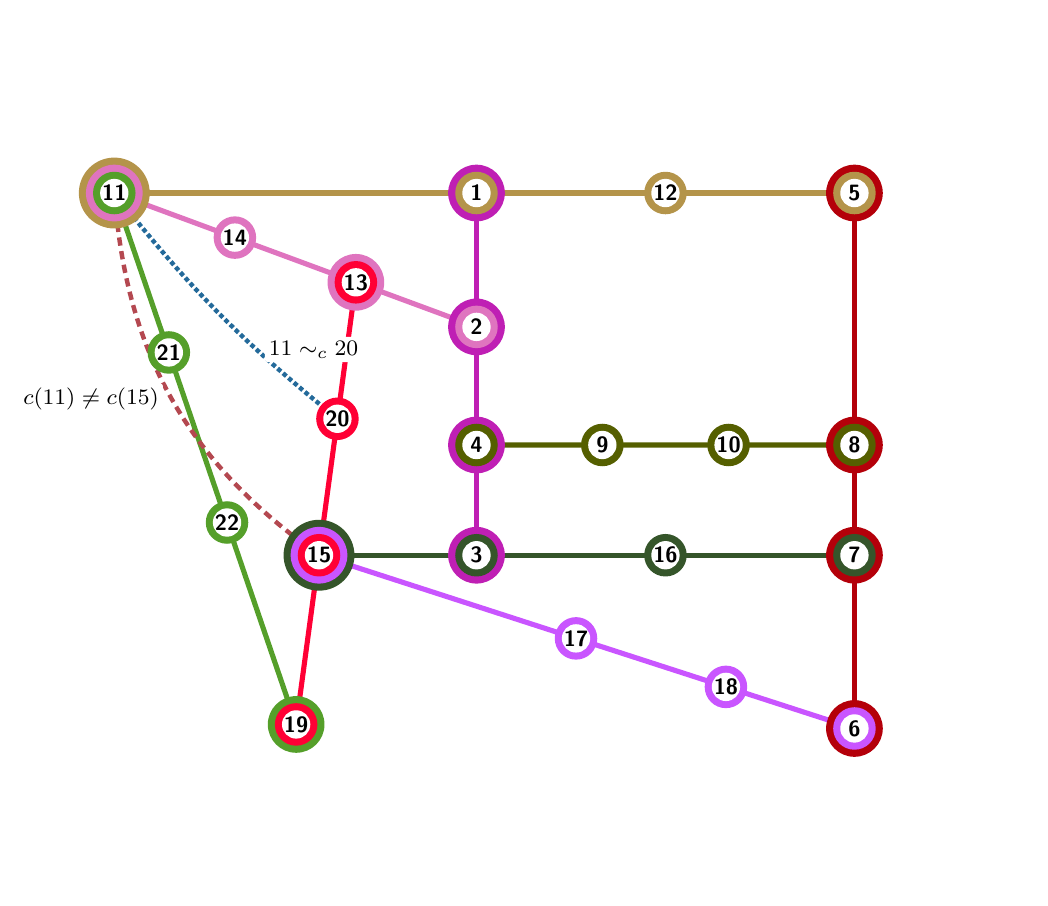
\begin{tikzpicture}[x=1cm,y=1cm]
    % Base 7 straight-line contexts C1..C7 (identical to Panel d):
    \coordinate (v1)  at (-0.60, 3.30);
    \coordinate (v2)  at (-0.60, 1.60);
    \coordinate (v4)  at (-0.60, 0.10);
    \coordinate (v3)  at (-0.60,-1.30);
    \coordinate (v5)  at ( 4.20, 3.30);
    \coordinate (v8)  at ( 4.20, 0.10);
    \coordinate (v7)  at ( 4.20,-1.30);
    \coordinate (v6)  at ( 4.20,-3.50);
    \coordinate (v9)  at ($(v4)!.333!(v8)$);
    \coordinate (v10) at ($(v4)!.667!(v8)$);
    \coordinate (v11) at (-5.20, 3.30);
    \coordinate (v12) at ($(v1)!.50!(v5)$);
    \coordinate (v14) at ($(v11)!.333!(v2)$);
    \coordinate (v13) at ($(v11)!.667!(v2)$);
    \coordinate (v15) at (-2.60,-1.30);
    \coordinate (v16) at ($(v3)!.50!(v7)$);
    \coordinate (v17) at ($(v15)!.48!(v6)$);
    \coordinate (v18) at ($(v15)!.76!(v6)$);
    % Two-context strictly linear TITS extension C8={11,21,22,19} and C9={13,20,15,19} as pure straight lines:
    \coordinate (v20) at ($(v13)!.50!(v15)$);
    \coordinate (v19) at ($(v13)!1.62!(v15)$);
    \coordinate (v21) at ($(v11)!.30!(v19)$);
    \coordinate (v22) at ($(v11)!.62!(v19)$);
    % Draw all 9 4-uniform contexts as pure straight lines (zero crossings!):
    \draw[YOtrace,YOctx1]  (v1)--(v2)--(v4)--(v3);
    \draw[YOtrace,YOctx2]  (v5)--(v8)--(v7)--(v6);
    \draw[YOtrace,YOctx4]  (v4)--(v9)--(v10)--(v8);
    \draw[YOtrace,YOctx8]  (v11)--(v1)--(v12)--(v5);
    \draw[YOtrace,YOctx9]  (v11)--(v14)--(v13)--(v2);
    \draw[YOtrace,YOctx11] (v15)--(v3)--(v16)--(v7);
    \draw[YOtrace,YOctx12] (v15)--(v17)--(v18)--(v6);
    \draw[YOtrace,YOctx5]  (v11)--(v21)--(v22)--(v19);
    \draw[YOtrace,YOctx16] (v13)--(v20)--(v15)--(v19);
    % Highlight TIFS c(11)!=c(15) and nonseparating TITS 11 ~_c 20
    \draw[CSexcl]  (v11) to[bend right=24] node[CSnote,pos=.50,anchor=east,xshift=-3pt] {$c(11)\ne c(15)$} (v15);
    \draw[CSident] (v11) to[bend right=6]  node[CSnote,pos=.68,anchor=west,xshift=2pt] {$11\sim_c 20$} (v20);
    \YOvertex{1}{1/.36,8/.27}
    \YOvertex{2}{1/.36,9/.27}
    \YOvertex{3}{1/.36,11/.27}
    \YOvertex{4}{1/.36,4/.27}
    \YOvertex{5}{2/.36,8/.27}
    \YOvertex{6}{2/.36,12/.27}
    \YOvertex{7}{2/.36,11/.27}
    \YOvertex{8}{2/.36,4/.27}
    \YOvertex{9}{4/.27}
    \YOvertex{10}{4/.27}
    \YOvertex{11}{8/.45,9/.36,5/.27}
    \YOvertex{12}{8/.27}
    \YOvertex{13}{9/.36,16/.27}
    \YOvertex{14}{9/.27}
    \YOvertex{15}{11/.45,12/.36,16/.27}
    \YOvertex{16}{11/.27}
    \YOvertex{17}{12/.27}
    \YOvertex{18}{12/.27}
    \YOvertex{19}{5/.36,16/.27}
    \YOvertex{20}{16/.27}
    \YOvertex{21}{5/.27}
    \YOvertex{22}{5/.27}
    \pgfresetboundingbox
    \path[use as bounding box] (-6.3,-5.4) rectangle (6.3,5.4);
  \end{tikzpicture}%
}
% END INLINED FILE: figures/chromatic-gadgets-4d.tex

\hypersetup{pdftitle={Chromatic Contextuality and Separability of Context Hypergraphs},pdfauthor={Karl Svozil}}
% BEGIN COMPANION LABEL SNAPSHOT
% Embedded labels of the companion manuscript; refreshed by build.py.
\makeatletter
\@namedef{r@S-FirstPage}{{}{1}{}{section*.1}{../supplement/2026-color-20p-supp.pdf}}
\@namedef{r@S-LastBibItem}{{10}{63}{}{section*.91}{../supplement/2026-color-20p-supp.pdf}}
\@namedef{r@S-LastPage}{{}{63}{}{}{../supplement/2026-color-20p-supp.pdf}}
\@namedef{r@S-app:all-states}{{S2}{25}{}{section*.34}{../supplement/2026-color-20p-supp.pdf}}
\@namedef{r@S-app:all-vectors}{{S1}{1}{}{section*.4}{../supplement/2026-color-20p-supp.pdf}}
\@namedef{r@S-app:cabello-proofs}{{S3\,S3.5}{60}{}{section*.86}{../supplement/2026-color-20p-supp.pdf}}
\@namedef{r@S-app:cabello-states}{{S2\,S2.30\,S2.30.1}{52}{}{section*.73}{../supplement/2026-color-20p-supp.pdf}}
\@namedef{r@S-app:cabello-vectors}{{S1\,S1.17\,S1.17.1}{19}{}{section*.31}{../supplement/2026-color-20p-supp.pdf}}
\@namedef{r@S-app:gadget-vectors}{{S1\,S1.2}{2}{}{section*.6}{../supplement/2026-color-20p-supp.pdf}}
\@namedef{r@S-app:historical}{{S3\,S3.9}{62}{}{section*.90}{../supplement/2026-color-20p-supp.pdf}}
\@namedef{r@S-app:historical-cert}{{S3\,S3.8}{62}{}{section*.89}{../supplement/2026-color-20p-supp.pdf}}
\@namedef{r@S-app:parent-states}{{S2\,S2.29}{51}{}{section*.71}{../supplement/2026-color-20p-supp.pdf}}
\@namedef{r@S-app:parents-vectors}{{S1\,S1.16}{14}{}{section*.26}{../supplement/2026-color-20p-supp.pdf}}
\@namedef{r@S-app:states}{{S2}{25}{}{section*.34}{../supplement/2026-color-20p-supp.pdf}}
\@namedef{r@S-app:supplementary}{{S3}{56}{}{section*.76}{../supplement/2026-color-20p-supp.pdf}}
\@namedef{r@S-app:transverse-certificates}{{S3\,S3.6}{61}{}{section*.87}{../supplement/2026-color-20p-supp.pdf}}
\@namedef{r@S-app:vec-3a}{{S1\,S1.3}{3}{}{section*.7}{../supplement/2026-color-20p-supp.pdf}}
\@namedef{r@S-app:vec-3b}{{S1\,S1.4}{3}{}{section*.8}{../supplement/2026-color-20p-supp.pdf}}
\@namedef{r@S-app:vec-3c}{{S1\,S1.5}{4}{}{section*.9}{../supplement/2026-color-20p-supp.pdf}}
\@namedef{r@S-app:vec-3d}{{S1\,S1.6}{4}{}{section*.10}{../supplement/2026-color-20p-supp.pdf}}
\@namedef{r@S-app:vec-3e}{{S1\,S1.7}{5}{}{section*.11}{../supplement/2026-color-20p-supp.pdf}}
\@namedef{r@S-app:vec-4a}{{S1\,S1.8}{5}{}{section*.12}{../supplement/2026-color-20p-supp.pdf}}
\@namedef{r@S-app:vec-4b}{{S1\,S1.9}{6}{}{section*.13}{../supplement/2026-color-20p-supp.pdf}}
\@namedef{r@S-app:vec-4c}{{S1\,S1.10}{6}{}{section*.14}{../supplement/2026-color-20p-supp.pdf}}
\@namedef{r@S-app:vec-4d}{{S1\,S1.11}{7}{}{section*.15}{../supplement/2026-color-20p-supp.pdf}}
\@namedef{r@S-app:vec-4e}{{S1\,S1.12}{7}{}{section*.16}{../supplement/2026-color-20p-supp.pdf}}
\@namedef{r@S-app:vec-4f}{{S1\,S1.13}{8}{}{section*.17}{../supplement/2026-color-20p-supp.pdf}}
\@namedef{r@S-app:vectors}{{S1}{1}{}{section*.4}{../supplement/2026-color-20p-supp.pdf}}
\@namedef{r@S-app:yo-vectors}{{S1\,S1.1}{2}{}{section*.5}{../supplement/2026-color-20p-supp.pdf}}
\@namedef{r@S-d:app:h65}{{S1\,S1.15\,S1.15.1}{11}{}{section*.24}{../supplement/2026-color-20p-supp.pdf}}
\@namedef{r@S-d:app:hyo4}{{S1\,S1.15\,S1.15.2}{13}{}{section*.25}{../supplement/2026-color-20p-supp.pdf}}
\@namedef{r@S-d:app:states-h65}{{S2\,S2.28\,S2.28.2}{49}{}{section*.70}{../supplement/2026-color-20p-supp.pdf}}
\@namedef{r@S-d:app:states-hyo4}{{S2\,S2.28\,S2.28.1}{48}{}{section*.69}{../supplement/2026-color-20p-supp.pdf}}
\@namedef{r@S-d:app:verification}{{S3\,S3.4}{60}{}{section*.85}{../supplement/2026-color-20p-supp.pdf}}
\@namedef{r@S-d:eq:canonical-primitive}{{S4}{10}{}{equation.4}{../supplement/2026-color-20p-supp.pdf}}
\@namedef{r@S-d:eq:canonical-state-supports}{{S21}{50}{}{equation.21}{../supplement/2026-color-20p-supp.pdf}}
\@namedef{r@S-d:eq:canonical-states}{{S29}{56}{}{equation.29}{../supplement/2026-color-20p-supp.pdf}}
\@namedef{r@S-d:eq:completion-score}{{S43}{60}{}{equation.43}{../supplement/2026-color-20p-supp.pdf}}
\@namedef{r@S-d:eq:full-state-param}{{S20}{50}{}{equation.20}{../supplement/2026-color-20p-supp.pdf}}
\@namedef{r@S-d:eq:h65-coordinates}{{S28}{56}{}{equation.28}{../supplement/2026-color-20p-supp.pdf}}
\@namedef{r@S-d:eq:hyo4-inclusions}{{S19}{48}{}{equation.19}{../supplement/2026-color-20p-supp.pdf}}
\@namedef{r@S-d:eq:hyo4-triad-disjoint}{{S18}{48}{}{equation.18}{../supplement/2026-color-20p-supp.pdf}}
\@namedef{r@S-d:eq:hyo4-vectors}{{S5}{13}{}{equation.5}{../supplement/2026-color-20p-supp.pdf}}
\@namedef{r@S-d:eq:plane-param}{{S30}{56}{}{equation.30}{../supplement/2026-color-20p-supp.pdf}}
\@namedef{r@S-d:tab:app-h65-contexts}{{S18}{12}{Complete enumeration of the $29$ four-element contexts of $H_{65}=(V_{65},E_{29})$, listing for each context both its vertex indices $\{i,j,k,\ell \}$ and the four mutually orthogonal unnormalized integer vectors $\{v_i,v_j,v_k,v_\ell \}\subset \mathbb {Z}^4$}{table.18}{../supplement/2026-color-20p-supp.pdf}}
\@namedef{r@S-d:tab:app-h65-state-branches}{{S81}{50}{Complete branch-by-branch parametrization of the $24\times 2^{14}=393{,}216$ two-valued states $s_{\alpha ,\bm {\varepsilon }}$ and the $48$ canonical states $s_{\alpha ,0},s_{\alpha ,1}$ on $H_{65}$ via Eqs.~\eqref {d:eq:full-state-param}--\eqref {d:eq:canonical-state-supports}. For each $\alpha \in \{1,\ldots ,24\}$, the table lists the $4$-element core support $S_\alpha $, the $10$ hit completion context indices $m\in \mathcal {H}_\alpha $ where $(s(2m+16),s(2m+17))=(0,0)$ is forced on $E_m$, the $14$ free completion context indices $m\in \mathcal {F}_\alpha $ where $(s(2m+16),s(2m+17))=(1-\varepsilon _m,\varepsilon _m)$ with $\varepsilon _m\in \{0,1\}$ on $E_m$, and the $24$-bit indicator string $(\mathbf {1}_{1\in \mathcal {F}_\alpha }\ldots \mathbf {1}_{12\in \mathcal {F}_\alpha }\,\mathbf {1}_{13\in \mathcal {F}_\alpha }\ldots \mathbf {1}_{24\in \mathcal {F}_\alpha })$}{table.81}{../supplement/2026-color-20p-supp.pdf}}
\@namedef{r@S-d:tab:app-h65-vectors}{{S17}{11}{Complete enumeration of the $65$ unnormalized integer vectors $v_i\in \mathbb {Z}^4$ of $H_{65}$, their squared norms $\|v_i\|^2$, their colors $c(i)\in \{0,1,2,3,4\}$, and the contexts in $E_{29}$ containing vertex $i$}{table.17}{../supplement/2026-color-20p-supp.pdf}}
\@namedef{r@S-d:tab:app-h65-vertex-profiles}{{S82}{51}{Vertex state profiles and weights for all $65$ vertices of $H_{65}$, showing for each core vertex $i\in \{1,\ldots ,17\}$ and each completion pair $(w_{m,1},w_{m,2})=(2m+16,2m+17)$ ($m=1,\ldots ,24$) the number of active branches $W_{24}$, the weight $W_{48}=\sum _{\alpha ,\varepsilon }s_{\alpha ,\varepsilon }(i)$ across the $48$ canonical states, the weight $W_{393{,}216}=\sum _{s\in \mathcal {S}(H_{65})}s(i)$ across all $393{,}216$ states, the active branch indices $\alpha \in \{1,\ldots ,24\}$ (equal to $Z(e_m)$ for $(w_{m,1},w_{m,2})$), and the $24$-bit branch profile across $S_1,\ldots ,S_{24}$ (in which each \texttt {1} expands to \texttt {11} for core vertices $i$, to \texttt {10} for $w_{m,1}$, and to \texttt {01} for $w_{m,2}$ across the $48$ canonical states)}{table.82}{../supplement/2026-color-20p-supp.pdf}}
\@namedef{r@S-d:tab:app-hyo4-contexts}{{S19}{13}{Complete enumeration of the $16$ four-element contexts of the non-linear warm-up apex suspension $H_{\YO }^{(4)}=(V_{26},E_{16}^{(4)})$, listing for each context both its vertex indices $\{i,j,k,26\}$ and the four mutually orthogonal unnormalized integer vectors $\{v_i,v_j,v_k,v_{26}\}\subset \mathbb {Z}^4$}{table.19}{../supplement/2026-color-20p-supp.pdf}}
\@namedef{r@S-d:tab:app-hyo4-profiles}{{S80}{49}{Vertex state profiles across the $25$ two-valued states $s_1,\ldots ,s_{25}$ of $H_{\YO }^{(4)}$, showing for each vertex $i\in \{1,\ldots ,26\}$ its state weight $\sum _{r=1}^{25}s_r(i)$, the active state indices $\{r : s_r(i)=1\}$, and the $25$-bit profile $(s_{1\ldots 12}(i)\,s_{13\ldots 24}(i)\,s_{25}(i))$. All $26$ rows are nonzero and pairwise distinct}{table.80}{../supplement/2026-color-20p-supp.pdf}}
\@namedef{r@S-d:tab:app-hyo4-states}{{S79}{48}{Complete enumeration of the $25$ two-valued states $s_1,\ldots ,s_{25}:V_{26}\to \{0,1\}$ on the non-linear warm-up hypergraph $H_{\YO }^{(4)}=(V_{26},E_{16}^{(4)})$, showing for each state its support on the $13$-ray Yu--Oh core $\{1,\ldots ,13\}$, its forced support on $\{14,\ldots ,26\}$, its total support size $|S_r|$, and its $26$-bit binary vector $(s_r(1\ldots 13)\,s_r(14\ldots 25)\,s_r(26))$}{table.79}{../supplement/2026-color-20p-supp.pdf}}
\@namedef{r@S-eq:cabello-nine-pairs}{{S32}{56}{}{equation.32}{../supplement/2026-color-20p-supp.pdf}}
\@namedef{r@S-eq:cabello-published-map}{{S6}{21}{}{equation.6}{../supplement/2026-color-20p-supp.pdf}}
\@namedef{r@S-eq:cabello45-state-counts}{{S22}{54}{}{equation.22}{../supplement/2026-color-20p-supp.pdf}}
\@namedef{r@S-eq:i16}{{S33}{56}{}{equation.33}{../supplement/2026-color-20p-supp.pdf}}
\@namedef{r@S-eq:ks1965}{{S44}{62}{}{equation.44}{../supplement/2026-color-20p-supp.pdf}}
\@namedef{r@S-eq:yo-parent-eight}{{S31}{56}{}{equation.31}{../supplement/2026-color-20p-supp.pdf}}
\@namedef{r@S-h:app:branches}{{S2\,S2.27\,S2.27.1}{41}{}{section*.62}{../supplement/2026-color-20p-supp.pdf}}
\@namedef{r@S-h:app:minimal-families}{{S3\,S3.3}{59}{}{section*.82}{../supplement/2026-color-20p-supp.pdf}}
\@namedef{r@S-h:app:order-determination}{{S2\,S2.27\,S2.27.6}{47}{}{section*.67}{../supplement/2026-color-20p-supp.pdf}}
\@namedef{r@S-h:app:separating}{{S2\,S2.27\,S2.27.3}{45}{}{section*.64}{../supplement/2026-color-20p-supp.pdf}}
\@namedef{r@S-h:app:states}{{S2\,S2.27}{41}{}{section*.61}{../supplement/2026-color-20p-supp.pdf}}
\@namedef{r@S-h:app:vectors-contexts}{{S1\,S1.14}{8}{}{section*.18}{../supplement/2026-color-20p-supp.pdf}}
\@namedef{r@S-h:eq:app-cover-family}{{S16}{47}{}{equation.16}{../supplement/2026-color-20p-supp.pdf}}
\@namedef{r@S-h:eq:app-max-overlap}{{S2}{10}{}{equation.2}{../supplement/2026-color-20p-supp.pdf}}
\@namedef{r@S-h:eq:app-six-states}{{S15}{45}{}{equation.15}{../supplement/2026-color-20p-supp.pdf}}
\@namedef{r@S-h:eq:canonical-profile}{{S26}{56}{}{equation.26}{../supplement/2026-color-20p-supp.pdf}}
\@namedef{r@S-h:eq:eighteen-order-family}{{S25}{56}{}{equation.25}{../supplement/2026-color-20p-supp.pdf}}
\@namedef{r@S-h:eq:order-witness-set}{{S42}{59}{}{equation.42}{../supplement/2026-color-20p-supp.pdf}}
\@namedef{r@S-h:eq:pasting-order}{{S27}{56}{}{equation.27}{../supplement/2026-color-20p-supp.pdf}}
\@namedef{r@S-h:eq:seven-separating}{{S24}{56}{}{equation.24}{../supplement/2026-color-20p-supp.pdf}}
\@namedef{r@S-h:eq:seventeen-search-count}{{S41}{59}{}{equation.41}{../supplement/2026-color-20p-supp.pdf}}
\@namedef{r@S-h:eq:six-separating}{{S23}{56}{}{equation.23}{../supplement/2026-color-20p-supp.pdf}}
\@namedef{r@S-h:tab:app-branches}{{S73}{42}{All 27 state branches. The sets $U(t),W(t)$ identify the free core bits. The two choices of $\varepsilon $ give $N_0=2^{|U|+|W|}$ and $N_1=2^{|W|}$ states; their index ranges refer to Table~\ref {h:tab:app-states}}{table.73}{../supplement/2026-color-20p-supp.pdf}}
\@namedef{r@S-h:tab:app-contexts}{{S16}{9}{All 24 orthogonal triads, numbered in the same order as the context colors in Fig.~\ref {M-h:fig:hesse37-hypergraph}. Vectors are given in increasing order of their vertex numbers. Each triad contributes three orthogonality edges; the 72 resulting pairs are all the orthogonal pairs}{table.16}{../supplement/2026-color-20p-supp.pdf}}
\@namedef{r@S-h:tab:app-double-cover}{{S78}{47}{Explicit six-state double cover $\mathcal R_6$. Omitted $P,Q$ values are zero; completion values follow from the state equations}{table.78}{../supplement/2026-color-20p-supp.pdf}}
\@namedef{r@S-h:tab:app-full-profiles}{{S77}{46}{Complete 153-bit vertex profiles, with consecutive 51-bit blocks. Every row is nonzero and all 37 rows are distinct}{table.77}{../supplement/2026-color-20p-supp.pdf}}
\@namedef{r@S-h:tab:app-six-profiles}{{S76}{46}{All 37 vertex profiles on $\Omega _6$, in two panels. Here $X_i^{(6)}=\{j:\sigma _j(i)=1\}$, $W_6=|X_i^{(6)}|$, and $W_{153}$ is the weight across the full state space. The six-bit rows are nonzero and pairwise distinct}{table.76}{../supplement/2026-color-20p-supp.pdf}}
\@namedef{r@S-h:tab:app-six-states}{{S75}{45}{Complete supports and state vectors of the minimum unital, separating family $\Omega _6$. The full state indices are those of Table~\ref {h:tab:app-states}}{table.75}{../supplement/2026-color-20p-supp.pdf}}
\@namedef{r@S-h:tab:app-states}{{S74}{43}{Canonical enumeration of all 153 two-valued states, in the canonical order defined above. The support is split into core and completion vertices. The last column is $(s_r(1),\ldots ,s_r(16)\,;\,s_r(17),\ldots ,s_r(37))$}{table.74}{../supplement/2026-color-20p-supp.pdf}}
\@namedef{r@S-h:tab:app-vectors}{{S15}{8}{Complete enumeration of the 37 vectors of $H_{37}$. The color $c(i)\in \{0,1,2,3\}$ is the explicit four-coloring in the main text. Context indices refer to Table~\ref {h:tab:app-contexts}}{table.15}{../supplement/2026-color-20p-supp.pdf}}
\@namedef{r@S-h:tab:pair-witnesses}{{S91}{59}{Complete joint-one witness classes for the fifteen pairs in $D$. Each entry lists all canonical indices $r$ for which $s_r(u)=s_r(v)=1$}{table.91}{../supplement/2026-color-20p-supp.pdf}}
\@namedef{r@S-m:app:states}{{S2\,S2.26}{40}{}{section*.60}{../supplement/2026-color-20p-supp.pdf}}
\@namedef{r@S-m:cor:snarks}{{1}{57}{Obstruction for Blanu\v {s}a and dot-product snarks}{theorem.1}{../supplement/2026-color-20p-supp.pdf}}
\@namedef{r@S-m:eq:approx-parseval}{{S38}{58}{}{equation.38}{../supplement/2026-color-20p-supp.pdf}}
\@namedef{r@S-m:eq:approx-proj}{{S39}{58}{}{equation.39}{../supplement/2026-color-20p-supp.pdf}}
\@namedef{r@S-m:eq:delta3-bounds}{{S36}{57}{Quantitative bounds on $\Delta _3$}{equation.36}{../supplement/2026-color-20p-supp.pdf}}
\@namedef{r@S-m:eq:epsilon-bound}{{S35}{57}{Quantitative bounds on $\Delta _3$}{equation.35}{../supplement/2026-color-20p-supp.pdf}}
\@namedef{r@S-m:eq:robustness}{{S34}{57}{}{equation.34}{../supplement/2026-color-20p-supp.pdf}}
\@namedef{r@S-m:eq:state-extension}{{S7}{40}{}{equation.7}{../supplement/2026-color-20p-supp.pdf}}
\@namedef{r@S-m:eq:tetrahedral-orbit}{{S40}{58}{}{equation.40}{../supplement/2026-color-20p-supp.pdf}}
\@namedef{r@S-m:eq:tetrahedral-poly}{{S37}{58}{Quantitative bounds on $\Delta _3$}{equation.37}{../supplement/2026-color-20p-supp.pdf}}
\@namedef{r@S-m:eq:yo-profiles}{{S8}{41}{}{equation.8}{../supplement/2026-color-20p-supp.pdf}}
\@namedef{r@S-m:prop:robustness}{{2}{57}{Quantitative bounds on $\Delta _3$}{theorem.2}{../supplement/2026-color-20p-supp.pdf}}
\@namedef{r@S-m:sec:directions}{{S3\,S3.2}{57}{}{section*.79}{../supplement/2026-color-20p-supp.pdf}}
\@namedef{r@S-m:tab:yo-states}{{S72}{40}{The 24 states are indexed by $(k,b)$, where $1\le k\le 12$ and $b\in \{0,1\}$. Their support on vertices $1,\ldots ,13$ is $T_k$ when $b=0$ and $T_k\cup \{\eta _k\}$ when $b=1$. Equation~\eqref {m:eq:state-extension} determines all remaining values}{table.72}{../supplement/2026-color-20p-supp.pdf}}
\@namedef{r@S-tab:bub49-contexts}{{S21}{15}{All 36 complete bases of the real parent}{table.21}{../supplement/2026-color-20p-supp.pdf}}
\@namedef{r@S-tab:bub49-vectors}{{S20}{14}{All unnormalized vectors of the real 49-ray parent, with the verified published Bub labels}{table.20}{../supplement/2026-color-20p-supp.pdf}}
\@namedef{r@S-tab:cabello-context-deletions}{{S87}{54}{All single-context deletion counts and four-coloring witnesses for $C_{18,9}$}{table.87}{../supplement/2026-color-20p-supp.pdf}}
\@namedef{r@S-tab:cabello-eight-context-states}{{S88}{54}{All 26 states after deleting context 9; geometric compatibility is marked explicitly}{table.88}{../supplement/2026-color-20p-supp.pdf}}
\@namedef{r@S-tab:cabello-published-map}{{S30}{21}{Exact ray map from the originally published Cabello coordinates}{table.30}{../supplement/2026-color-20p-supp.pdf}}
\@namedef{r@S-tab:cabello-vertex-deletions}{{S89}{55}{All eighteen vertex-deletion checks; the completed geometric families fail unitality and separation in every case}{table.89}{../supplement/2026-color-20p-supp.pdf}}
\@namedef{r@S-tab:cabello20-ray-criticality}{{S90}{55}{Geometric state counts after every single-ray deletion of the twenty-ray parity subsystem}{table.90}{../supplement/2026-color-20p-supp.pdf}}
\@namedef{r@S-tab:cabello36-contexts}{{S29}{21}{All eighteen full bases of the faithful Cabello completion}{table.29}{../supplement/2026-color-20p-supp.pdf}}
\@namedef{r@S-tab:cabello36-vectors}{{S28}{20}{All 36 unnormalized vectors of the faithful Cabello completion}{table.28}{../supplement/2026-color-20p-supp.pdf}}
\@namedef{r@S-tab:cabello45-canonical}{{S86}{53}{All 24 canonical context-state supports of the 45-ray example. Some fail geometric pair exclusions}{table.86}{../supplement/2026-color-20p-supp.pdf}}
\@namedef{r@S-tab:cabello45-contexts}{{S32}{23}{All 21 full bases of the vertex-deleted completion}{table.32}{../supplement/2026-color-20p-supp.pdf}}
\@namedef{r@S-tab:cabello45-core-states}{{S84}{53}{All twelve core supports; $m=|F_\alpha |$. The final column specifies extendibility under all geometric pair exclusions}{table.84}{../supplement/2026-color-20p-supp.pdf}}
\@namedef{r@S-tab:cabello45-vectors}{{S31}{22}{All 45 unnormalized vectors of the vertex-deleted completion}{table.31}{../supplement/2026-color-20p-supp.pdf}}
\@namedef{r@S-tab:cabello45-zero-profiles}{{S85}{53}{The fourteen bridge pairs, fresh labels, and zero-profiles; each $Z_m$ is the set of missed-bridge branch indices}{table.85}{../supplement/2026-color-20p-supp.pdf}}
\@namedef{r@S-tab:cabello68-1-contexts}{{S34}{24}{All 35 full bases of 68-ray parent variant 1}{table.34}{../supplement/2026-color-20p-supp.pdf}}
\@namedef{r@S-tab:cabello68-2-contexts}{{S35}{24}{All 35 full bases of 68-ray parent variant 2}{table.35}{../supplement/2026-color-20p-supp.pdf}}
\@namedef{r@S-tab:cabello68-rays}{{S33}{23}{The three added rays in each local 68-ray parent inventory}{table.33}{../supplement/2026-color-20p-supp.pdf}}
\@namedef{r@S-tab:chromatic-signatures}{{S44}{27}{The nine chromatic signatures of $H_{21,13}$. Columns give $c_1$ and rows give $c_2$ for the two normalized colorings in Table~\ref {tab:h21-colors}. Each cell is one inseparability class: its vertices have the same color in every admissible coloring. Ordinary two-valued states distinguish every pair, including vertices in the same cell}{table.44}{../supplement/2026-color-20p-supp.pdf}}
\@namedef{r@S-tab:colors-3a}{{S58}{33}{Every normalized coloring of $P_5$}{table.58}{../supplement/2026-color-20p-supp.pdf}}
\@namedef{r@S-tab:colors-3b}{{S59}{33}{Every normalized coloring of $B_{13,7}$}{table.59}{../supplement/2026-color-20p-supp.pdf}}
\@namedef{r@S-tab:colors-3c}{{S60}{34}{Every normalized coloring of $D_{16,9}$}{table.60}{../supplement/2026-color-20p-supp.pdf}}
\@namedef{r@S-tab:colors-3d}{{S61}{34}{Every normalized coloring of $I_{16,9}$}{table.61}{../supplement/2026-color-20p-supp.pdf}}
\@namedef{r@S-tab:colors-3e}{{S62}{34}{Every normalized coloring of $T_{19,11}$}{table.62}{../supplement/2026-color-20p-supp.pdf}}
\@namedef{r@S-tab:colors-3f}{{S63}{34}{Every normalized coloring of $H_{21,13}$}{table.63}{../supplement/2026-color-20p-supp.pdf}}
\@namedef{r@S-tab:colors-4a}{{S64}{35}{Every normalized coloring of $W_{11,5}^{(4)}$}{table.64}{../supplement/2026-color-20p-supp.pdf}}
\@namedef{r@S-tab:colors-4b}{{S65}{35}{Every normalized coloring of $W_{16,6}^{(4)}$}{table.65}{../supplement/2026-color-20p-supp.pdf}}
\@namedef{r@S-tab:colors-4c}{{S66}{36}{Every normalized coloring of $B_{14,7}^{(4)}$}{table.66}{../supplement/2026-color-20p-supp.pdf}}
\@namedef{r@S-tab:colors-4d}{{S67}{36}{Every normalized coloring of $L_{18,7}^{(4)}$}{table.67}{../supplement/2026-color-20p-supp.pdf}}
\@namedef{r@S-tab:colors-4e}{{S68}{37}{Every normalized coloring of $D_{17,9}^{(4)}$}{table.68}{../supplement/2026-color-20p-supp.pdf}}
\@namedef{r@S-tab:colors-4f}{{S69}{38}{Every normalized coloring of $L_{22,9}^{(4)}$}{table.69}{../supplement/2026-color-20p-supp.pdf}}
\@namedef{r@S-tab:contexts}{{S3}{3}{The 16 parent contexts and the two selected restrictions}{table.3}{../supplement/2026-color-20p-supp.pdf}}
\@namedef{r@S-tab:deletion-colorings}{{S92}{61}{Explicit deletion colorings with pattern (1,1,2) and the number of states after deleting the corresponding first-copy horizontal context}{table.92}{../supplement/2026-color-20p-supp.pdf}}
\@namedef{r@S-tab:h17-colors}{{S41}{26}{All strong three-colorings of $H_{17,10}$ up to color permutation. The anchor is $(2,8,5)=(0,1,2)$}{table.41}{../supplement/2026-color-20p-supp.pdf}}
\@namedef{r@S-tab:h17-states}{{S40}{26}{All two-valued states of $H_{17,10}$. The last column gives an odd cycle in the complement of each nonextendable support}{table.40}{../supplement/2026-color-20p-supp.pdf}}
\@namedef{r@S-tab:h21-colors}{{S43}{27}{All strong three-colorings of $H_{21,13}$ up to color permutation. The anchor is $(2,8,5)=(0,1,2)$}{table.43}{../supplement/2026-color-20p-supp.pdf}}
\@namedef{r@S-tab:h21-states}{{S42}{26}{All two-valued states of $H_{21,13}$. The last column gives an odd cycle in the complement of each nonextendable support}{table.42}{../supplement/2026-color-20p-supp.pdf}}
\@namedef{r@S-tab:h6-states}{{S36}{25}{All two-valued states of $H_{6,3}$. The last column gives an odd cycle in the complement of each nonextendable support}{table.36}{../supplement/2026-color-20p-supp.pdf}}
\@namedef{r@S-tab:h8-colors}{{S39}{25}{All strong three-colorings of $H_8$ up to color permutation. The anchor is $(1,2,3)=(0,1,2)$}{table.39}{../supplement/2026-color-20p-supp.pdf}}
\@namedef{r@S-tab:h8-states}{{S38}{25}{All two-valued states of $H_8$. The last column gives an odd cycle in the complement of each nonextendable support}{table.38}{../supplement/2026-color-20p-supp.pdf}}
\@namedef{r@S-tab:hesse87-contexts}{{S23}{17}{All 64 complete bases of the first 87-ray Hesse parent}{table.23}{../supplement/2026-color-20p-supp.pdf}}
\@namedef{r@S-tab:hesse87-vectors}{{S22}{15}{All 87 unnormalized rays of the first Hesse/lineage union}{table.22}{../supplement/2026-color-20p-supp.pdf}}
\@namedef{r@S-tab:inventory}{{S71}{40}{All ten connected, edge-faithful, colorable restrictions with a forced color identity in the specified inventory}{table.71}{../supplement/2026-color-20p-supp.pdf}}
\@namedef{r@S-tab:p5-states}{{S37}{25}{All two-valued states of $P_5$. The last column gives an odd cycle in the complement of each nonextendable support}{table.37}{../supplement/2026-color-20p-supp.pdf}}
\@namedef{r@S-tab:parent-added-rays}{{S25}{18}{Every ray added to the original four-dimensional examples to obtain the stated parents}{table.25}{../supplement/2026-color-20p-supp.pdf}}
\@namedef{r@S-tab:parent-criticality}{{S83}{52}{State counts after deleting each single context of the real 49-ray parent. Every count is positive. Context numbering is Table~\ref {tab:bub49-contexts}}{table.83}{../supplement/2026-color-20p-supp.pdf}}
\@namedef{r@S-tab:parent40-contexts}{{S26}{19}{All 36 complete bases of the 40-ray parent}{table.26}{../supplement/2026-color-20p-supp.pdf}}
\@namedef{r@S-tab:parent72-contexts}{{S27}{19}{All 48 complete bases of the 72-ray parent}{table.27}{../supplement/2026-color-20p-supp.pdf}}
\@namedef{r@S-tab:peres-all}{{S24}{17}{All 24 primitive unnormalized Peres rays, in the certificate order}{table.24}{../supplement/2026-color-20p-supp.pdf}}
\@namedef{r@S-tab:profiles}{{S45}{27}{Complete state profiles in hexadecimal, and all Born probabilities for the 17-ray preparation in Eq.~\eqref {M-eq:rho}. The probabilities are also reproduced by Eq.~\eqref {M-eq:mixture}}{table.45}{../supplement/2026-color-20p-supp.pdf}}
\@namedef{r@S-tab:pure-witnesses}{{S70}{40}{Ordinary states violating each directed truth implication for color-identical terminals. Both witness patterns and all context normalizations are verified}{table.70}{../supplement/2026-color-20p-supp.pdf}}
\@namedef{r@S-tab:quantum}{{S46}{28}{The five valid states and exact weights reproducing the $H_{17,10}$ preparation $P_{24}$. State numbering is that of Table~\ref {tab:h17-states}. Every context equation and every Born marginal are checked with rational arithmetic}{table.46}{../supplement/2026-color-20p-supp.pdf}}
\@namedef{r@S-tab:quantum-probabilities}{{S47}{28}{Exact Born probabilities $p_i=(r_{24}\cdot r_i)^2/(6\|r_i\|^2)$, also reproduced by the five-state mixture}{table.47}{../supplement/2026-color-20p-supp.pdf}}
\@namedef{r@S-tab:states-3b}{{S48}{28}{All two-valued states of $B_{13,7}$. E indicates extendability}{table.48}{../supplement/2026-color-20p-supp.pdf}}
\@namedef{r@S-tab:states-3c}{{S49}{28}{All two-valued states of $D_{16,9}$. E indicates extendability}{table.49}{../supplement/2026-color-20p-supp.pdf}}
\@namedef{r@S-tab:states-3d}{{S50}{29}{All two-valued states of $I_{16,9}$. E indicates extendability}{table.50}{../supplement/2026-color-20p-supp.pdf}}
\@namedef{r@S-tab:states-3e}{{S51}{29}{All two-valued states of $T_{19,11}$. E indicates extendability}{table.51}{../supplement/2026-color-20p-supp.pdf}}
\@namedef{r@S-tab:states-4a}{{S52}{29}{All two-valued states of $W_{11,5}^{(4)}$. E indicates extendability}{table.52}{../supplement/2026-color-20p-supp.pdf}}
\@namedef{r@S-tab:states-4b}{{S53}{30}{All two-valued states of $W_{16,6}^{(4)}$. E indicates extendability}{table.53}{../supplement/2026-color-20p-supp.pdf}}
\@namedef{r@S-tab:states-4c}{{S54}{30}{All two-valued states of $B_{14,7}^{(4)}$. E indicates extendability}{table.54}{../supplement/2026-color-20p-supp.pdf}}
\@namedef{r@S-tab:states-4d}{{S55}{31}{All two-valued states of $L_{18,7}^{(4)}$. E indicates extendability}{table.55}{../supplement/2026-color-20p-supp.pdf}}
\@namedef{r@S-tab:states-4e}{{S56}{31}{All two-valued states of $D_{17,9}^{(4)}$. E indicates extendability}{table.56}{../supplement/2026-color-20p-supp.pdf}}
\@namedef{r@S-tab:states-4f}{{S57}{32}{All two-valued states of $L_{22,9}^{(4)}$. E indicates extendability}{table.57}{../supplement/2026-color-20p-supp.pdf}}
\@namedef{r@S-tab:vec-3a}{{S4}{3}{Unnormalized vectors and all contexts of $P_5$}{table.4}{../supplement/2026-color-20p-supp.pdf}}
\@namedef{r@S-tab:vec-3b}{{S5}{3}{Unnormalized vectors and all contexts of $B_{13,7}$}{table.5}{../supplement/2026-color-20p-supp.pdf}}
\@namedef{r@S-tab:vec-3c}{{S6}{4}{Unnormalized vectors and all contexts of $D_{16,9}$}{table.6}{../supplement/2026-color-20p-supp.pdf}}
\@namedef{r@S-tab:vec-3d}{{S7}{4}{Unnormalized vectors and all contexts of $I_{16,9}$}{table.7}{../supplement/2026-color-20p-supp.pdf}}
\@namedef{r@S-tab:vec-3e}{{S8}{5}{Unnormalized vectors and all contexts of $T_{19,11}$}{table.8}{../supplement/2026-color-20p-supp.pdf}}
\@namedef{r@S-tab:vec-4a}{{S9}{5}{Unnormalized vectors and all contexts of $W_{11,5}^{(4)}$}{table.9}{../supplement/2026-color-20p-supp.pdf}}
\@namedef{r@S-tab:vec-4b}{{S10}{6}{Unnormalized vectors and all contexts of $W_{16,6}^{(4)}$}{table.10}{../supplement/2026-color-20p-supp.pdf}}
\@namedef{r@S-tab:vec-4c}{{S11}{6}{Unnormalized vectors and all contexts of $B_{14,7}^{(4)}$}{table.11}{../supplement/2026-color-20p-supp.pdf}}
\@namedef{r@S-tab:vec-4d}{{S12}{7}{Unnormalized vectors and all contexts of $L_{18,7}^{(4)}$}{table.12}{../supplement/2026-color-20p-supp.pdf}}
\@namedef{r@S-tab:vec-4e}{{S13}{7}{Unnormalized vectors and all contexts of $D_{17,9}^{(4)}$}{table.13}{../supplement/2026-color-20p-supp.pdf}}
\@namedef{r@S-tab:vec-4f}{{S14}{8}{Unnormalized vectors and all contexts of $L_{22,9}^{(4)}$}{table.14}{../supplement/2026-color-20p-supp.pdf}}
\@namedef{r@S-tab:vectors}{{S2}{2}{All 25 unnormalized parent vectors; membership of the two geometric examples}{table.2}{../supplement/2026-color-20p-supp.pdf}}
\@namedef{r@S-tab:yo-all-vectors}{{S1}{2}{All 25 unnormalized completed Yu--Oh vectors}{table.1}{../supplement/2026-color-20p-supp.pdf}}
\@namedef{r@S-tab:yo-core-vectors}{{S2}{2}{All 25 unnormalized parent vectors; membership of the two geometric examples}{table.2}{../supplement/2026-color-20p-supp.pdf}}
\makeatother
% END COMPANION LABEL SNAPSHOT
\begin{document}
\title{Chromatic Contextuality and Separability of Context Hypergraphs}
\author{Karl Svozil\,\orcidlink{0000-0001-6554-2802}}
\email{karl.svozil@tuwien.ac.at}
\affiliation{Institute for Theoretical Physics, TU Wien, Wiedner Hauptstra{\ss}e 8-10/136, A-1040 Vienna, Austria}
\date{Integrated draft for author review --- October 26, 2026}
\begin{abstract}
Intertwined complete projective experiments share outcomes, motivating the search for a common spectral labeling across contexts. Strong coloring tests whether complete contexts admit one context-independent nondegenerate spectrum; when that labeling exists, chromatic separability tests which event distinctions it preserves. We distinguish these questions from ordinary Kochen--Specker statelessness, geometric realizability, event-order representation, and Born-probability models. A state extends to a strong $d$-coloring exactly when deletion of its support leaves a $(d-1)$-colorable graph. Faithful real 17- and 21-ray restrictions of completed Yu--Oh have separating ordinary states but forced color identities; one quantum preparation requires exactly $1/9$ nonextendable weight despite admitting an ordinary-state model. Independent Hermitian projection arguments correct earlier inferences from a chromatic gap to statelessness or nonrealizability. Hesse's complex 37-ray example separates real and complex geometry and has exact state-family minima $6/7/18$ for three representation requirements. A rational two-plane construction gives a linear real 65-ray example with 393,216 states and explicit event-order and probability failures. General and specified ancestry results distinguish geometric KS extensions from abstract chromatic-to-stateless constructions. Detailed enumerations, regenerated state certificates, and extended proofs are supplementary.
\end{abstract}
\maketitle
% BEGIN INLINED FILE: sections/01-introduction.tex
\section{Introduction}\label{sec:intro}

An experimental context with $d$ rank-one outcomes admits a nondegenerate observable with $d$ distinct eigenvalues. These eigenvalues distinguish all $d$ outcomes and provide the maximal resolution of a complete projective experiment within that context. Such an observable is maximal in the sense that every self-adjoint observable commuting with it is a function of it, so the statistics of the latter can be obtained by processing its measurement outcomes. Noninjective functions merge outcomes and reduce this resolution. This is the finite-dimensional setting of von Neumann's functional representation of commuting observables~\cite[Satz~8, p.~221]{v-neumann-31}; see also Halmos~\cite[\S84, pp.~171--172]{halmos-vs}.

When complete experiments are intertwined, they share outcomes represented by the same rank-one projectors. The physical motivation is to ask whether these maximally resolved experiments admit a globally consistent labeling of their outcomes by one common nondegenerate spectrum. Each individual context admits a maximal observable, but consistency across the family requires the same projector to carry the same spectral label wherever it occurs. This additional common-spectrum requirement is explicit: if context-dependent labels are allowed, a shared projector can carry different eigenvalues in different observables.

A two-valued state retains only the distinction between one selected outcome and the remaining outcomes. A uniform coloring must retain all $d$ distinct spectral values simultaneously. It therefore demands more than a single classical truth assignment. Even when such a complete labeling exists, its consistency across intertwined contexts can impose relations between distinct outcomes that are absent from the full family of individual truth assignments. We study both the existence of a uniform spectral labeling and the event distinctions and logical relations that survive when such labelings are available~\cite{svozil-2020-c,svozil-2021-chroma,svozil-2025-color}.

To express these questions, let a $d$-uniform context hypergraph $H=(V,E)$ encode the complete experiments. An ordinary two-valued state $s:V\to\{0,1\}$ selects exactly one outcome in every context, so $\sum_{v\in e}s(v)=1$ for every $e\in E$. The Kochen--Specker (KS) theorem~\cite{kochen1} establishes the nonexistence of such a global truth assignment for suitable finite families of intertwined projective contexts in dimension $d\ge3$.

A strong $d$-coloring $c:V\to\{0,\ldots,d-1\}$ assigns all $d$ distinct labels bijectively within every context and independently of context at shared vertices. For an injective ray realization $i\mapsto[v_i]\in\PP(\F^d)$, with $\F\in\{\R,\C\}$, rank-one projectors $P_i$, and a common nondegenerate real spectrum $\Sigma=\{\lambda_0,\ldots,\lambda_{d-1}\}$, it defines the maximal context observables
\begin{equation}\label{eq:intro-maximal-obs}
A_e=\sum_{i\in e}\lambda_{c(i)}P_i.
\end{equation}

Because the indicator functions $s_a(v)=\mathbf 1_{\{c(v)=a\}}$ ($a\in\{0,\ldots,d-1\}$) of any strong $d$-coloring form $d$ two-valued states whose supports partition $V$, one has the strict one-way implication
\begin{equation}\label{eq:intro-ks-to-chi}
\mathcal S(H)=\varnothing \quad\Longrightarrow\quad \chi(H)>d,
\end{equation}
whose converse fails even when $\mathcal S(H)$ is unital and separates every pair of vertices. The earlier introduction in Ref.~\cite{svozil-2021-chroma} inferred absence of global two-valued assignments from $\chi>d$. Equation~\eqref{eq:intro-ks-to-chi} is the valid implication; completed Yu--Oh refutes the converse. The distinct Appendix~B inference about geometry is corrected below. We use ``exact palette'' for $\chi(H)=d$; this is the agreed meaning of ``tight'' here, with no additional density or geometric assumption. This asymmetry separates chromatic contextuality into two distinct regimes that are unified in this work:

\begin{enumerate}
\item \emph{Common-spectrum chromatic obstructions ($\chi(H)>d$, possibly with $\mathcal S(H)\ne\varnothing$):} Here no strong $d$-coloring exists ($\mathcal C_d(H)=\varnothing$), ruling out a context-independent common $d$-element spectral labeling, including examples in which classical truth assignments survive. A critical foundational clarification—correcting an interpretation in Appendix~B of the earlier work with Shekarriz~\cite{svozil-2021-chroma}—is that the chromatic obstruction $\chi(H)>d$ is an operator spectral-value obstruction and \emph{does not} by itself obstruct geometric ray realizability in $\F^d$. Indeed, for finite $3$-uniform linear hypergraphs of Berge girth five with unital separating state spaces, strong $3$-colorability and injective $\C^3$ realizability are logically independent (Proposition~\ref{m:prop:independence}). Ruling out geometric ray assignments for Greechie's Petersen-derived $G_{32}$~\cite{greechie:71} requires a direct Hermitian projection-identity argument (Theorem~\ref{m:thm:multipole}) rather than $\chi(G_{32})=4$.
\item \emph{Exact-palette chromatic separability and logical gadgets ($\chi(H)=d$ with $\mathcal S_{\mathrm{ext}}(H)\subsetneq\mathcal S(H)$):} Even when $\mathcal C_d(H)\ne\varnothing$, not every two-valued state $s\in\mathcal S(H)$ can be completed to a strong $d$-coloring. We characterize the extendable states $\mathcal S_{\mathrm{ext}}(H)$ by the residual chromatic condition $\chi(\Gamma(H)[V\setminus\supp s])\le d-1$ (Theorem~\ref{thm:completion}), which in dimension $d=3$ yields an odd-cycle nonextendability certificate. In the specified subhypergraphs—such as the faithful real $17$-ray and $21$-ray restrictions $H_{17,10}$ and $H_{21,13}$ of completed Yu--Oh~\cite{Yu-2012,svozil-2025-color} (Theorems~\ref{thm:h17} and~\ref{thm:h21}) and our faithful $3$- and $4$-dimensional logical gadgets (Secs.~\ref{sec:3dgadgets} and~\ref{sec:4dgadgets})—ordinary states separate all vertices while every admissible $d$-coloring forces nonadjacent rays to share a color ($u\sim_c v$, chromatic inseparability / implicit identity~\cite{martin2009}) or obeys purely chromatic true-implies-false (TIFS) or ternary exclusions violated by nonextendable states in $\mathcal S(H)\setminus\mathcal S_{\mathrm{ext}}(H)$.
\end{enumerate}

These two regimes are governed by a shared structural mechanism. Lemma~\ref{lem:disjoint-states} ($\chi(H)=d$ if and only if $H$ admits $d-1$ pairwise disjoint states) is the global unanchored form of Theorem~\ref{thm:completion}. Likewise, the eight normalized $3$-colorings of the four base contexts of completed Yu--Oh $H_{\YO}^+$ partition into four antipodal pairs that each make one of the four diagonal neighborhoods rainbow (Theorem~\ref{m:thm:yo-criticality}): retaining all four diagonal sectors forces $\chi(H_{\YO}^+)=4$ (Regime~I), whereas retaining two or three sectors leaves four or two normalized $3$-colorings and forces two or $21$ chromatically inseparable pairs in $H_{17,10}$ and $H_{21,13}$ (Regime~II), which our exhaustive $65{,}535$-subset inventory classification (Proposition~\ref{prop:search}) proves minimal within $H_{\YO}^+$.

We further connect these combinatorial and geometric layers to orthomodular event representations and quantum probability polytopes $\mathcal P_{\mathrm{ext}}(H)\subseteq\mathcal P(H)=\conv\mathcal S(H)$. On $H_{17,10}$, an explicit quantum ray preparation lies in $\mathcal P(H_{17,10})\setminus\mathcal P_{\mathrm{ext}}(H_{17,10})$ and requires nonextendable state weight at least $1/9$ (Theorem~\ref{thm:quantum}). In complex dimension three, the $37$-ray Hesse restriction $H_{37}$~\cite{svozil-2025-MYOCHS} has no injective $\R^3$ realization, pastes into a $76$-event orthomodular lattice with exact minimum state-family sizes $6$, $7$, and $18$ for vertex separation, event separation, and order determination (Theorem~\ref{h:thm:main}), and demonstrates that exact event-order determination does not guarantee classical mixtures for all Born preparations (Corollary~\ref{cor:order-probabilities}). In real dimension four, our two-plane completion lemma (Lemma~\ref{d:lem:plane-completion}) produces the canonical linear $65$-ray hypergraph $H_{65}$ completing the $17$-ray core of Haynes \emph{et al.}~\cite{haynes2010orthogonal} with $\chi=5$, $\chi_f=17/4$, and $393{,}216$ states that fail atom-order determination and collapse a ray with a plane (Theorem~\ref{d:thm:h65}). Finally, we formulate and prove the existence form of the KS ancestry hypothesis (Proposition~\ref{prop:ks-ancestry}), give an abstract transverse chromatic-to-stateless construction (Proposition~\ref{prop:transverse}), establish exact inclusions into specified KS parents (Bub's $49$-ray set, the $165$-ray MUB inventory, Peres's $24$-ray geometry, and $68$-ray extensions containing Cabello's $C_{18,9}$ and $C_{20,11}$ parity proofs), and contrast abstract context states $\mathcal S_{\mathrm{ctx}}$ with geometric states $\mathcal S_{\mathrm{geom}}$ on Cabello's $36$-ray completion and $45$-ray vertex deletion. Complete vector, state, and coloring enumerations and finite verification certificates are provided in the Supplemental Material~\cite{supplement}.
% END INLINED FILE: sections/01-introduction.tex

% BEGIN INLINED FILE: sections/02-framework.tex
\section{Unified Framework: States, Colorings, Separability, and Completion}\label{sec:definitions}

\subsection{Context hypergraphs, orthogonal realizations, and spectral regimes}

All hypergraphs and graphs considered here are finite. A $d$-uniform \emph{context hypergraph} $H=(V,E)$ ($d\ge2$) consists of a nonempty collection $E$ of $d$-element subsets of $V$, called \emph{contexts}, with $V=\bigcup_{e\in E}e$. Its \emph{two-section} (or \emph{context}) \emph{graph} $\Gamma(H)$ has vertex set $V$ and edge set $E(\Gamma(H))=\bigcup_{e\in E}\binom{e}{2}$. A hypergraph $H$ is \emph{linear} if $|e\cap e'|\le 1$ for all distinct $e,e'\in E$. A \emph{Berge cycle} of length $\ell\ge2$ is an alternating sequence of distinct vertices $x_1,\ldots,x_\ell$ and distinct contexts $e_1,\ldots,e_\ell$ with $\{x_j,x_{j+1}\}\subseteq e_j$ cyclically; the least such $\ell$ is the \emph{Berge girth} $g(H)$ (or $\infty$ if acyclic). In Greechie's pasting of Boolean blocks~\cite{greechie:71,svozil-tkadlec}, linearity ($g(H)\ge3$) with $g(H)\ge4$ yields an \emph{orthomodular poset}, and $g(H)\ge5$ yields an \emph{orthomodular lattice} (OML).

With the Hermitian inner product $\ip{x}{y}=\sum_j\overline{x_j}y_j$ on $\F^d$ ($\F\in\{\R,\C\}$), we distinguish three levels of geometric realization:
\begin{enumerate}
\item An \emph{orthogonal ray assignment} $\rho:V\to\PP(\F^d)$, $i\mapsto[v_i]$ ($v_i\ne0$), requires $\ip{v_i}{v_j}=0$ whenever $i\sim j$ in $\Gamma(H)$; nonadjacent vertices may share a ray.
\item An \emph{injective orthogonal representation} additionally requires $[v_i]\ne[v_j]$ for all $i\ne j$.
\item An injective representation is \emph{edge-faithful} (abbreviated FOR) if $\ip{v_i}{v_j}=0 \iff i\sim j$ in $\Gamma(H)$ for all $i\ne j$~\cite{hogben2017orthogonal}.
\end{enumerate}

A \emph{strong $k$-coloring} of $H$ is a map $c:V\to\{0,\ldots,k-1\}$ injective on every context $e\in E$, i.e., a proper $k$-coloring of $\Gamma(H)$; the least such $k$ is $\chi(H)=\chi(\Gamma(H))$. We call $H$ \emph{chromatically complete} when $\chi(H)=d$ and write $\Cc_d(H)$ for the set of strong $d$-colorings of $H$. For a realized $d$-uniform hypergraph with rank-one projectors $P_i=v_iv_i^\dagger/\ip{v_i}{v_i}$, three spectral-labeling regimes arise: (i) \emph{context-dependent common spectrum}, where bijections $\ell_e:e\to\Sigma=\{\lambda_0,\ldots,\lambda_{d-1}\}$ define $A_e=\sum_{i\in e}\ell_e(i)P_i$ with shared projectors carrying context-dependent eigenvalues; (ii) \emph{context-independent vertex labeling} via a strong $k$-coloring $c$ and distinct real scalars $\lambda_0,\ldots,\lambda_{k-1}$ in Eq.~\eqref{eq:intro-maximal-obs}, where spectra vary across contexts whenever $|c(V)|>d$ (unavoidable when $\chi(H)>d$); and (iii) \emph{chromatic completeness} ($k=d$), which provides both context-independent eigenvalues and a single $d$-element spectrum $\Sigma$ for all $A_e$.

\subsection{Two-valued states, color extendability, and the separation hierarchy}

A \emph{two-valued context state} is a function $s:V\to\{0,1\}$ satisfying
\begin{equation}\label{eq:states}
\sum_{v\in e}s(v)=1\qquad(e\in E).
\end{equation}
We write $\Sc(H)=\Sc_{\mathrm{ctx}}(H)$ for the set of context states. For a ray realization $\rho$, the \emph{geometric state space}
\begin{equation}\label{eq:geometric-state-space}
\begin{aligned}
\Sc_{\rm geom}(H,\rho)=\{s\in\Sc(H):{}&s(i)+s(j)\le1\\
&\text{whenever }i\ne j,\ v_i\perp v_j\}.
\end{aligned}
\end{equation}
additionally enforces orthogonality exclusions on uncovered pairs~\cite{waegell2011peres}; $\Sc_{\mathrm{geom}}(H,\rho)=\Sc(H)$ when $\rho$ is edge-faithful. A state family $\Omega\subseteq\Sc(H)$ is \emph{unital} if every $v\in V$ has $s(v)=1$ for some $s\in\Omega$, and \emph{vertex separating} if distinct $u,v\in V$ have $s(u)\ne s(v)$ for some $s\in\Omega$, inducing the partition set representation $A_i=\{s\in\Omega:s(i)=1\}$. On an event poset $(L,\le)$, $\Omega$ is \emph{event separating} if distinct $x,y\in L$ have distinct profiles on $\Omega$, and \emph{order determining} if $x\le y \iff (\forall s\in\Omega,\ s(x)\le s(y))$.

\begin{definition}[Chromatic separability and extendable states]\label{def:inseparable}
For chromatically complete $H$ ($\Cc_d(H)\ne\varnothing$), vertices $u,v\in V$ are \emph{chromatically inseparable}, written $u\sim_c v$, if
\begin{equation}\label{eq:inseparable}
c(u)=c(v)\qquad\text{for every }c\in\Cc_d(H),
\end{equation}
an \emph{implicit identity} in graph coloring~\cite[Def.~3.8]{martin2009}. We call $H$ \emph{chromatically separating} if $u\sim_c v\implies u=v$. A state $s\in\Sc(H)$ is \emph{extendable}, written $s\in\Sc_{\mathrm{ext}}(H)$, if $\supp s=\{v\in V:s(v)=1\}$ is a color class of some $c\in\Cc_d(H)$~\cite{svozil-2020-c,svozil-2021-chroma,svozil-2025-color}.
\end{definition}

\begin{theorem}[Completion criterion]\label{thm:completion}
For $s\in\Sc(H)$ with $S=\supp s$, the following are equivalent:
\begin{enumerate}
\item $s\in\Sc_{\mathrm{ext}}(H)$;
\item $\chi(\Gamma(H)[V\setminus S])\le d-1$ (so $S$ is a critical independent set~\cite[Def.~3.3]{martin2009});
\item $s$ belongs to $d$ states in $\Sc(H)$ with pairwise disjoint supports partitioning $V$;
\item $s$ belongs to $d-1$ states in $\Sc(H)$ with pairwise disjoint supports.
\end{enumerate}
For $d=3$, $s\notin\Sc_{\mathrm{ext}}(H)$ if and only if $\Gamma(H)[V\setminus S]$ contains an odd cycle.
\end{theorem}
\begin{proof}
A strong $d$-coloring with color class $S$ leaves a $(d-1)$-coloring on $V\setminus S$. Conversely, any $(d-1)$-coloring of $\Gamma(H)[V\setminus S]$ combined with a $d$th color on $S$ is a strong $d$-coloring because each context meets $S$ once and forms a $(d-1)$-clique in $V\setminus S$; its color indicators yield (3). Trivially (3)$\implies$(4), and given $d-1$ disjoint state supports $S_1,\ldots,S_{d-1}$, the complement $s_d(v)=1-\sum_{k=1}^{d-1}s_k(v)$ is binary and sums to $d-(d-1)=1$ on every context, giving (3). For $d=3$, $\chi(\Gamma(H)[V\setminus S])\le 2$ holds if and only if $\Gamma(H)[V\setminus S]$ is bipartite (odd-cycle free).
\end{proof}

Applying the equivalence (3)$\iff$(4) of Theorem~\ref{thm:completion} globally without anchoring a state $s$ yields the characterization of chromatic completeness:

\begin{lemma}[Disjoint states and strong coloring]\label{lem:disjoint-states}
A finite $d$-uniform hypergraph $H$ satisfies $\chi(H)=d$ if and only if $\Sc(H)$ contains $d-1$ states with pairwise disjoint supports.
\end{lemma}

\begin{corollary}[The separation hierarchy]\label{cor:hierarchy}
For chromatically complete $H$ and $u,v\in V$,
\begin{equation}\label{eq:kernel}
u\sim_c v \quad\Longleftrightarrow\quad s(u)=s(v)\text{ for all }s\in\Sc_{\mathrm{ext}}(H).
\end{equation}
Thus inseparability by $\Sc(H)$ implies chromatic inseparability ($\sim_c$), and chromatic separation implies separation by $\Sc(H)$, whereas the converse fails even for faithful real ray configurations. Moreover, $\Sc_{\mathrm{ext}}(H)$ is always unital whenever $\Cc_d(H)\ne\varnothing$.
\end{corollary}
\begin{proof}
The indicator states $s_a(v)=\mathbf 1_{\{c(v)=a\}}$ over all $c\in\Cc_d(H)$ and $a\in\{0,\ldots,d-1\}$ are precisely $\Sc_{\mathrm{ext}}(H)$, which partitions $V$ for any single $c\in\Cc_d(H)$ and satisfies $\Sc_{\mathrm{ext}}(H)\subseteq\Sc(H)$.
\end{proof}

\begin{proposition}[Canonical chromatic quotient and closure test]\label{prop:quotient}\label{prop:closure}
Let $H$ be chromatically complete.
\begin{enumerate}
\item The relation $\sim_c$ is an equivalence relation with no two equivalent vertices in a common context. The quotient $\overline H=(V/{\sim_c},\overline E)$ is $d$-uniform and chromatically separating, and pullback along $V\to V/{\sim_c}$ induces a bijection $\Cc_d(\overline H)\to\Cc_d(H)$.
\item For $u\ne v$, adjoining one context $\{u,v,w_1,\ldots,w_{d-2}\}$ with fresh vertices $w_i$ yields chromatic number $d+1$ if and only if $u\sim_c v$, and $d$ otherwise. Consequently, the \emph{separable chromatic number}~\cite{svozil-2020-c} of any nontrivial graph satisfies $\chi_{\mathrm{sep}}\in\{\chi,\chi+1\}$.
\end{enumerate}
\end{proposition}
\begin{proof}
(1) Adjacent vertices receive distinct colors, so each context projects injectively to $V/{\sim_c}$, and every $c\in\Cc_d(H)$ factors uniquely through $V/{\sim_c}$. (2) A coloring $c\in\Cc_d(H)$ extends to the fresh context if and only if $c(u)\ne c(v)$; if $u\sim_c v$, recoloring $u$ with a $(d+1)$th color separates $(u,v)$ while preserving all old context inequalities.
\end{proof}

The quotient preserves colorings, not an injective realization. Closing an inseparable pair is likewise abstract: faithful coordinates make the pair nonorthogonal, so the added context cannot retain those rays.

Put $\mathcal P_{\mathrm{ext}}=\conv\mathcal S_{\mathrm{ext}}$ and $\mathcal P=\conv\mathcal S$. A binary vector cannot be a convex combination of distinct binary vectors, since each positive-weight term must agree at every coordinate. Consequently,
\begin{equation}\label{eq:polytope-equality}
\mathcal P_{\mathrm{ext}}=\mathcal P\quad\Longleftrightarrow\quad\mathcal S_{\mathrm{ext}}=\mathcal S.
\end{equation}
This is stronger than equality of vertex-separation kernels: the pentagon has separating colors yet a nonextendable state. Pair identities alone do not describe all completion constraints.

\subsection{Fractional coloring and fresh-vertex context completion}

Write $\alpha(G)$ for the independence number and $\chi_f(G)$ for the fractional chromatic number of $G=\Gamma(H)$.

\begin{proposition}[Fractional threshold and uniform state mixture]\label{prop:fractional-uniform}
For any finite $d$-uniform context hypergraph $H$,
\begin{equation}\label{eq:fractional-uniform}
\chi_f(\Gamma(H))=d \quad\Longleftrightarrow\quad \frac1d\mathbf 1\in\mathcal P(H)=\conv\Sc(H).
\end{equation}
\end{proposition}
\begin{proof}
A state mixture $\sum_{s\in\Sc(H)}\mu_s s=\frac1d\mathbf 1$ assigns weight $d\mu_s$ to the independent set $\supp s$, covering each vertex with weight $1$ at total weight $d\ge\omega(\Gamma(H))\ge d$. Conversely, a fractional coloring $\{w_I\}$ of total weight $d$ obeys $d\le\sum_{v\in e}\sum_{I\ni v}w_I=\sum_I w_I|I\cap e|\le\sum_I w_I=d$ for each $e\in E$, forcing $|I\cap e|=1$ whenever $w_I>0$, so $\{w_I/d\}$ is a state mixture equal to $\frac1d\mathbf 1$.
\end{proof}

\begin{proposition}[Fresh-vertex context completion]\label{prop:completion}
Let $G$ be a finite core graph with designated $d$-clique base contexts ($d\ge3$). Complete selected uncovered edges $\{u,v\}$ into $d$-cliques using $d-2$ degree-one fresh vertices per edge, covering all core vertices and edges. For the resulting hypergraph $H$ and $G'=\Gamma(H)$,
\begin{equation}\label{eq:completion-chi}
\begin{aligned}
\chi(G')&=\max\{d,\chi(G)\},\\
\chi_f(G')&=\max\{d,\chi_f(G)\},\\
|\Sc(H)|&=\sum_{S}(d-2)^{m(S)}.
\end{aligned}
\end{equation}
where $S$ ranges over independent core supports meeting each base context once and $m(S)$ counts completed edges missed by $S$.
\end{proposition}
\begin{proof}
Any $k$-coloring ($k\ge d$) or measurable fractional palette of size $k=\max\{d,\chi_f(G)\}$ assigns disjoint colors/sets of measure $1$ to $u$ and $v$, leaving $k-2\ge d-2$ colors (or measure $k-2\ge d-2$) for the $d-2$ fresh vertices. A core support $S$ hitting $\{u,v\}$ forces its fresh vertices to $0$, whereas a missed edge allows $d-2$ choices of a single fresh vertex set to $1$.
\end{proof}

% BEGIN INLINED FILE: tables/main-overview.tex
\begin{table*}[t]
\centering\small\setlength{\tabcolsep}{3pt}
\caption{Principal configurations. FOR means injective and edge-faithful; $g$ is Berge girth. Counts refer to all context states and all color-class states.}\label{tab:joint-comparison}
\begin{tabular}{p{.17\textwidth}rrrrrrrp{.35\textwidth}}\toprule
Configuration & $d$ & $|V|/|E|$ & $g$ & $\chi$ & $\chi_f$ & $|\Sc|$ & $|\Sc_{\mathrm{ext}}|$ & Geometry and principal distinction\\\midrule
One triad & 3 & 3/1 & $\infty$ & 3 & $3$ & 3 & 3 & Real FOR; colors separate.\\
$H_{6,3}$ & 3 & 6/3 & $3$ & 3 & $3$ & 4 & 3 & No injective complex realization.\\
$P_5$ & 3 & 10/5 & $5$ & 3 & $3$ & 11 & 10 & Real FOR; colors separate; ternary exclusion.\\
$H_8$ & 3 & 14/8 & $5$ & 3 & $3$ & 11 & 7 & Repeated-ray assignments; no complex injection.\\
$H_9$ & 3 & 15/9 & $5$ & 4 & $3$ & 8 & 0 & No complex ray assignment; context-critical.\\
$G_{32}$ & 3 & 15/10 & $5$ & 4 & $3$ & 6 & 0 & No complex ray assignment.\\
$H_{17,10}$ & 3 & 17/10 & $5$ & 3 & $3$ & 18 & 10 & Real FOR; two color-identical pairs.\\
$H_{21,13}$ & 3 & 21/13 & $5$ & 3 & $3$ & 21 & 6 & Real FOR; 21 color-identical pairs.\\
Completed Yu--Oh & 3 & 25/16 & $5$ & 4 & $35/11$ & 24 & 0 & Real FOR; context-critical.\\
$H_{37}$ & 3 & 37/24 & $5$ & 4 & $3$ & 153 & 0 & Complex FOR; no real injection; OML minima $6/7/18$.\\
$H_{\YO}^{(4)}$ & 4 & 26/16 & $2$ & 5 & $46/11$ & 25 & 0 & Real FOR; common-apex suspension, nonlinear.\\
$C_{36,18}$ & 4 & 36/18 & $3$ & 5 & $9/2$ & 0 & 0 & Faithful linear KS completion.\\
$H_{65}$ & 4 & 65/29 & $3$ & 5 & $17/4$ & 393,216 & 0 & Real FOR; false atom order and compound collapse.\\
\bottomrule\end{tabular}
\end{table*}
% END INLINED FILE: tables/main-overview.tex


The logical situation has two distinct branches. If a hypergraph has no admissible two-valued context state, it cannot admit a strong $d$-coloring, because the color classes of such a coloring would supply $d$ admissible states. The converse implication fails: a common-spectrum labeling may be impossible while ordinary states, including a unital separating family, remain available.

When a strong $d$-coloring does exist, its color classes provide a nonempty unital family of extendable states inside the full context-state space. A particular ordinary state belongs to this restricted family precisely when deleting its support leaves a $(d-1)$-colorable graph. Chromatic identities describe pairs having equal values in every state of that restricted family, and need not hold throughout the ordinary state space. These assignment questions have to be distinguished from the separate requirements of an injective geometric realization, a representation of event order, and a classical mixture reproducing a specified Born probability vector.
% END INLINED FILE: sections/02-framework.tex

% BEGIN INLINED FILE: sections/03-independence-petersen.tex
\section{Independence of Coloring and Coordinatization, Petersen Obstructions, and Completed Yu--Oh}\label{sec:independence}

\subsection{Small abstract examples and four-quadrant independence}

The non-linear hypergraph $H_{4,2}$ with contexts $\{1,2,3\}$ and $\{1,2,4\}$ has three states $\{1\}$, $\{2\}$, $\{3,4\}$ (all extendable), forces $3\sim_c 4$ and $s(3)=s(4)$, and has no injective $\C^3$ realization because two orthogonal rays determine a unique orthogonal-complement ray.

\begin{proposition}[Smallest linear chromatically inseparable hypergraph]\label{prop:six}
The linear $3$-uniform hypergraph $H_{6,3}$ with contexts $\{1,2,3\}$, $\{3,4,5\}$, $\{5,6,1\}$ of Berge girth three has four unital separating states $\{1,4\}$, $\{2,5\}$, $\{3,6\}$, $\{2,4,6\}$, a unique strong $3$-coloring up to permutation with inseparable classes $\{1,4\}$, $\{2,5\}$, $\{3,6\}$, and three extendable states (as $V\setminus\{2,4,6\}=\{1,3,5\}$ is a triangle). No linear $3$-uniform hypergraph with $|V|<6$ or $|E|<3$ has a chromatically inseparable pair, and $H_{6,3}$ admits no injective realization in $\C^3$.
\end{proposition}
\begin{proof}
The triangle $\{1,3,5\}$ in $\Gamma(H_{6,3})$ forces three distinct colors on $1,3,5$, whence $c(4)=c(1)$, $c(2)=c(5)$, and $c(6)=c(3)$. Similarly, in $\C^3$, $\{v_1,v_3,v_5\}$ forms an orthonormal basis, forcing $[v_4]=[v_1]$, $[v_2]=[v_5]$, and $[v_6]=[v_3]$. With $|E|\le2$, independent permutations of unshared vertices separate all pairs; by inclusion--exclusion, three linear $3$-contexts require $|V|\ge 6$.
\end{proof}

\begin{proposition}[Clique number at Berge girth at least four]\label{m:prop:ranks}
If $H=(V,E)$ is an $n$-uniform linear hypergraph ($n\ge3$) of Berge girth $g(H)\ge4$, every clique $K\subseteq V$ of size $|K|\ge3$ in $\Gamma(H)$ is contained in a unique context $e\in E$. Hence $\omega(\Gamma(H))=n$, and chromatic incompleteness ($\chi(H)>n$) is equivalent to the chromatic--clique gap $\chi(\Gamma(H))>\omega(\Gamma(H))$.
\end{proposition}
\begin{proof}
For any three vertices $u,v,w\in K$, pairwise adjacency gives contexts $e_1\supseteq\{u,v\}$, $e_2\supseteq\{v,w\}$, $e_3\supseteq\{w,u\}$. Distinct $e_1,e_2,e_3$ would form a Berge $3$-cycle, contradicting $g(H)\ge4$. By linearity, the shared context $e$ containing $\{u,v,w\}$ is unique for $\{u,v\}$ and thus contains all of $K$.
\end{proof}

\begin{proposition}[Logical independence of coloring and coordinatization]\label{m:prop:independence}
For finite $3$-uniform context hypergraphs, all four combinations of chromatic completeness ($\chi(H)=3$) and injective coordinatizability in $\C^3$ occur even within the orthomodular-lattice admissible class of linear hypergraphs of Berge girth $g(H)\ge5$~\cite{greechie:71,svozil-tkadlec} with unital separating state spaces:
\begin{enumerate}
\item $\chi=3$, injectively realizable in $\R^3$: a single context $C_1=\{\{1,2,3\}\}$ (or $P_5,H_{17,10},H_{21,13}$);
\item $\chi=3$, not injectively realizable in $\C^3$: the $8$-context Petersen restriction $H_8$ (Theorem~\ref{m:thm:multipole});
\item $\chi=4$, edge-faithfully realizable in $\R^3$: completed Yu--Oh $H_{\YO}^{+}$ (Theorem~\ref{m:thm:yo-criticality});
\item $\chi=4$, admitting no orthogonal ray assignment in $\C^3$: Greechie's $G_{32}$ and $H_9$ (Theorems~\ref{m:thm:multipole} and~\ref{m:thm:g32}).
\end{enumerate}
\end{proposition}
Injectivity is essential to quadrant~(2): any strong $n$-coloring $c$ yields a noninjective ray assignment $i\mapsto[e_{c(i)+1}]\in\PP(\F^n)$. At Berge girth four (an orthomodular poset that is not a lattice), $E_\square=\{\{1,2,3\}$, $\{3,4,5\}$, $\{5,6,7\}$, $\{7,8,1\}\}$ also satisfies $\chi=3$ while forcing $[v_3]=[v_7]\perp\spanop(v_1,v_5)$ whenever $[v_1]\ne[v_5]$.

\subsection{Greechie's \texorpdfstring{$G_{32}$}{G32}, multipole forcing, and correction of the JMP spectral argument}\label{m:sec:g32}

Greechie's $G_{32}$~\cite[Fig.~6]{greechie:71} has $15$ vertices and ten contexts
\begin{equation}\label{m:eq:g32-blocks}
\begin{aligned}
E(G_{32})=\{&123,345,567,789,9\,10\,11,\\
&11\,12\,1,4\,10\,13,6\,12\,14,\\
&8\,2\,15,13\,14\,15\}.
\end{aligned}
\end{equation}
Each vertex lies in two contexts, so $G_{32}$ is dual to the Petersen graph $P$, $\Gamma(G_{32})=L(P)$, $\mathrm{Aut}(G_{32})\cong S_5$, and $\chi(G_{32})=\chi'(P)=4$. Its six two-valued state supports satisfy
\begin{equation}\label{m:eq:g32-states}
|\mathcal S(G_{32})|=6,\qquad |S_\alpha|=5,\qquad
|S_\alpha\cap S_\beta|=1\ (\alpha\ne\beta).
\end{equation}
give the $\binom{6}{2}=15$ two-element vertex profiles $B_i=\{\alpha:i\in S_\alpha\}$ and satisfy $|S_\alpha\cap S_\beta|=1$ ($\alpha\ne\beta$), excluding even two disjoint states and confirming $\chi(G_{32})=4$ by Lemma~\ref{lem:disjoint-states}.

In Appendix~B of Shekarriz and Svozil~\cite{svozil-2021-chroma}, the chromatic obstruction $\chi(G_{32})=4>3$ was invoked to argue against a $3$-dimensional realization of $G_{32}$. As Proposition~\ref{m:prop:independence} demonstrates via $H_{\YO}^{+}$ ($\chi=4$, yet faithfully realizable in $\R^3$), $\chi(H)>3$ rules out only a context-independent $3$-value spectral assignment, \emph{not} geometric rays. A genuine geometric exclusion requires the projection identity: for an orthonormal basis $\{x,y,z\}\subset\C^3$ with $u\perp x$ and $w\perp z$,
\begin{equation}\label{m:eq:projection-identity}
\ip{u}{w}=\ip{u}{y}\ip{y}{w}.
\end{equation}

\begin{theorem}[Multipole forcing and minimal complex obstructions]\label{m:thm:multipole}\label{m:thm:g32}
Let $H_8=G_{32}\setminus\{\{8,2,15\}$, $\{13,14,15\}\}$ ($14$ vertices, $8$ contexts) and $H_9=G_{32}\setminus\{\{13,14,15\}\}$ ($15$ vertices, $9$ contexts).
\begin{enumerate}
\item In every orthogonal ray assignment of $H_8$ in $\C^3$ (allowing repeated rays), the terminal rays satisfy
\begin{equation}\label{m:eq:multipole-forcing}
[v_2]=[v_8]\qquad\text{and}\qquad [v_{13}]=[v_{14}],
\end{equation}
and either $[v_1]=[v_4]=[v_9]$ or $[v_3]=[v_7]=[v_{12}]$. Thus $H_8$ has no injective realization in $\C^3$.
\item $H_8$ is chromatically complete ($\chi(H_8)=3$) with $11$ unital separating states, of which $7$ are extendable (the $4$ nonextendable states leave odd cycles in $\Gamma(H_8)$; the corresponding supplemental table). Its $3$ normalized $3$-colorings (fixing $(c(1),c(2),c(3))=(0,1,2)$) are listed in Table~\ref{S-tab:h8-colors}, forcing the $6$ chromatically inseparable pairs $(1,9)$, $(2,8)$, $(3,7)$, $(4,6)$, $(10,12)$, $(13,14)$; deleting any single context of $H_8$ removes all forced color identities (leaving $6,20,20,6,20,20,6,6$ normalized colorings).
\item Neither $H_9$, $G_{32}$, nor the $12$-vertex, $21$-edge subgraph $\Gamma_0$ of $\Gamma(H_9)$ on $\{1,\ldots,12\}$ admits any orthogonal ray assignment in $\C^3$. Moreover, $H_9$ is context-minimal and $\Gamma_0$ is edge-minimal: deleting any context of $H_9$ or edge of $\Gamma_0$ yields a $3$-colorable structure realizable in $\R^3$ by standard basis rays.
\end{enumerate}
\end{theorem}
\begin{proof}
(1) Let $v_1,\ldots,v_{14}\in\C^3$ be unit vectors for $H_8$. In $\{v_1,v_2,v_3\}$, $v_{11},v_{12}\perp v_1$ and $v_4,v_5\perp v_3$, so Eq.~\eqref{m:eq:projection-identity} gives $\ip{x}{y}=\ip{x}{v_2}\ip{v_2}{y}$ for $x\in\{v_{11},v_{12}\},y\in\{v_4,v_5\}$. Expanding $v_{12}$ in $\{v_5,v_6,v_7\}$ ($v_{12}\perp v_6$) and $v_4$ in $\{v_9,v_{10},v_{11}\}$ ($v_4\perp v_{10}$) yields $v_7\ip{v_7}{v_{12}}=v_{12}-v_5\ip{v_5}{v_{12}}$ and $v_9\ip{v_9}{v_4}=v_4-v_{11}\ip{v_{11}}{v_4}$. Since $v_7\perp v_9$, $v_{12}\perp v_{11}$, and $v_5\perp v_4$, their inner product vanishes:
\begin{equation}\label{m:eq:coordfree-product}
\begin{aligned}
0={}&\ip{v_{12}}{v_4}
+\ip{v_{12}}{v_5}\ip{v_5}{v_{11}}\ip{v_{11}}{v_4}\\
={}&\ip{v_{12}}{v_2}\ip{v_2}{v_4}
\bigl(1+|\ip{v_2}{v_5}|^2|\ip{v_2}{v_{11}}|^2\bigr).
\end{aligned}
\end{equation}
Thus $\ip{v_2}{v_4}=0$ or $\ip{v_{12}}{v_2}=0$. If $\ip{v_2}{v_4}=0$, set $(v_1,v_3,v_2)=(e_1,e_2,e_3)$; then $v_4\perp v_2,v_3\implies[v_4]=[e_1]$, $\{3,4,5\}\implies[v_5]=[e_3]=[v_2]$, $\{9,10,11\}$ with $v_{10},v_{11}\perp e_1$ forces $[v_9]=[e_1]$, $\{5,6,7\}$ and $\{7,8,9\}$ force $[v_7]=[e_2],[v_6]=[e_1],[v_8]=[e_3]=[v_2]$, and $\{4,10,13\}$, $\{9,10,11\}$, $\{11,12,1\}$, $\{6,12,14\}$ in $\spanop(e_2,e_3)$ force $[v_{13}]=[v_{11}]=[v_{14}]$ and $[v_1]=[v_4]=[v_9]$. Reflection symmetry gives the second branch when $\ip{v_{12}}{v_2}=0$.

(2) In $H_8$, fixing $(c(1),c(2),c(3))=(0,1,2)$ leaves $16$ choices along $345,567,789,9\,10\,11$, of which $13$ fail on $11\,12\,1,4\,10\,13,6\,12\,14$, leaving $c_1,c_2,c_3$ in Table~\ref{S-tab:h8-colors}. Equal columns identify the $6$ pairs.

(3) Both $H_9$ (hence $G_{32}$) and $\Gamma_0$ add the orthogonality $v_2\perp v_8$ to $H_8$, contradicting $[v_2]=[v_8]$. For minimality, deleting $\{8,2,15\}$ from $H_9$ leaves $H_8$ ($\chi=3$); deleting $\{4,10,13\}$ or $\{6,12,14\}$ is isomorphic by $D_6$ symmetry to deleting $\{8,2,15\}$; and deleting any ring context (say $\{1,2,3\}$) allows the $3$-coloring $(c(1),\ldots,c(15))=(0,0,1,2,0,1,2,0,1,2,0,1,1,0,2)$. On $\Gamma_0$, the $21$ edges split into four $D_6$-orbits represented by $\{1,2\}$ (colored by $001201201201$), $\{2,3\}$ ($011201201201$), $\{1,3\}$ ($010210210201$), and $\{4,10\}$ ($012010210021$), each yielding a standard-basis $\R^3$ assignment $i\mapsto[e_{c(i)+1}]$. Quantitative robustness bounds $1/14400<\Delta_3<0.927496$ are proved in Supplement Sec.~S3.
\end{proof}

The complete normalized coloring lists for $H_8$ and $H_{17,10}$ are in the supplement.

\begin{corollary}[Blanu\v{s}a and Isaacs dot-product snarks]\label{m:cor:snarks}
If a cubic graph $G$ admits no orthogonal vector edge coloring in $\C^3$, neither does any Isaacs dot product $G\cdot P$~\cite{isaacs1975infinite}. In particular, both $18$-vertex Blanu\v{s}a snarks $B_1,B_2=P\cdot P$~\cite{blanusa1946problem} and all iterated dot products $X=P\cdot P\cdots P$ satisfy $\chi(H(X))=4>3=\omega(L(X))$ and admit no orthogonal ray assignment in $\C^3$.
\end{corollary}
\begin{proof}
In $G\cdot P$, the embedded copy of $P\setminus\{u,v\}$ has dual hypergraph $H_8$, so Theorem~\ref{m:thm:multipole}(1) forces $[v_2]=[v_8]$ and $[v_{13}]=[v_{14}]$ on the two pairs of cut edges, inducing a valid orthogonal ray assignment on $G$.
\end{proof}

\subsection{Completed Yu--Oh \texorpdfstring{$H_{\YO}^{+}$}{H\_YO\^+}, base-coloring partition, and context criticality}\label{m:sec:yuo}\label{m:sec:ranks}

Completing each of the $12$ uncovered orthogonal pairs of the $13$-ray Yu--Oh set~\cite{Yu-2012} ($r_1,\ldots,r_{13}\in\R^3$, consisting of $z_1=r_2,z_2=r_8,z_3=r_5$, $y_1^\pm=r_{1,3},y_2^\pm=r_{7,9},y_3^\pm=r_{4,6}$, and diagonals $h_0=r_{12},h_1=r_{11},h_2=r_{10},h_3=r_{13}$) by cross-product rays $r_{14},\ldots,r_{25}$ (Table~\ref{S-tab:yo-core-vectors}) yields the $25$-ray, $16$-context linear hypergraph $H_{\YO}^{+}$ of Berge girth five~\cite{Pavi_i__2019,svozil-2025-color}:
\begin{equation}\label{m:eq:yuo-blocks}
\begin{aligned}
E_{\YO}^{+}&=\{123,789,456,285\}\cup\bigcup_{h=10}^{13}\mathcal E_h,\\
\mathcal E_h&=\{\{x,h,w_{xh}\}:x\in N(h)\},
\end{aligned}
\end{equation}

All 25 vectors, 16 contexts, and restriction-membership flags are tabulated in the supplement.
Here the neighborhoods are $N(10)=\{1,9,4\}$, $N(11)=\{3,7,4\}$, $N(12)=\{3,9,6\}$ and $N(13)=\{1,7,6\}$, and each $w_{xh}$ is the unique completing ray. It has a real FOR in $\R^3$ ($48$ orthogonal pairs) and $24$ unital separating states (each of the $12$ binary assignments on the four base contexts leaves uniquely one diagonal $h_j$ with all three neighbors zero, allowing $s(h_j)\in\{0,1\}$ and hence $12+4\times3=24$ states).

\begin{theorem}[Base-coloring partition and context criticality of $H_{\YO}^{+}$]\label{m:thm:yo-criticality}\label{m:prop:fractional}
The completed Yu--Oh hypergraph $H_{\YO}^{+}$ satisfies $\omega(\Gamma(H_{\YO}^{+}))=3$, $\chi_f(\Gamma(H_{\YO}^{+}))=35/11>3=\chi_f(\Gamma(G_{32}))$, and $\chi(H_{\YO}^{+})=4$, and is context-critical for $\chi>3$:
\begin{enumerate}
\item Fixing $(c(2),c(8),c(5))=(0,1,2)$, the four base contexts $\{1,2,3\}$, $\{7,8,9\}$, $\{4,5,6\}$, $\{2,8,5\}$ admit eight strong $3$-colorings indexed by $(b_1,b_2,b_3)\in\{0,1\}^3$:
\begin{equation}\label{m:eq:yo-base-colorings}
\begin{aligned}
(c(1),c(3))&=(2-b_1,1+b_1),\\
(c(7),c(9))&=(2-2b_2,2b_2),\\
(c(4),c(6))&=(1-b_3,b_3).
\end{aligned}
\end{equation}
Each antipodal pair of $(b_1,b_2,b_3)$ makes the neighborhood $N(h_j)$ of \emph{uniquely one} diagonal ray $h_j\in\{10,11,12,13\}$ rainbow ($\{0,1,2\}$) while the other three neighborhoods are $2$-colored:
\begin{equation}\label{m:eq:yo-antipodal-pairs}
\begin{array}{c|c}
\text{Antipodal binary patterns}&\text{Blocked diagonal}\\\hline
101,010&12\\110,001&11\\000,111&10\\011,100&13
\end{array}
\end{equation}
\item Consequently, $\chi(H_{\YO}^{+})=4$, whereas deleting any single context $e\in E_{\YO}^{+}$ yields $\chi(H_{\YO}^{+}\setminus\{e\})=3$.
\end{enumerate}
\end{theorem}
\begin{proof}
Direct check of Eqs.~\eqref{m:eq:yo-base-colorings}--\eqref{m:eq:yo-antipodal-pairs} shows that every base $3$-coloring blocks one $h_j$, so $\chi(H_{\YO}^{+})\ge4$, matched by the explicit four-coloring in the supplementary vector table. Deleting a sector context $\{x,h_j,w\}$ frees $h_j$ in its antipodal base colorings by setting $c(h_j)=c(x)$; deleting $\{2,8,5\}$ allows $c(2)=c(8)=c(5)=0$; deleting $\{1,2,3\}$ allows $(c(1),c(2),c(3))=(0,0,1)$, $(c(7),c(8),c(9))=(2,1,0)$, $(c(4),c(5),c(6))=(1,2,0)$, and $(c(10),c(11),c(12),c(13))=(2,0,2,1)$. For $\chi_f$, weight $1/2$ on the $6$ states of $G_{32}$ gives $\chi_f(G_{32})=3$, while Proposition~\ref{prop:completion} preserves the $13$-ray value $\chi_f=35/11$~\cite{cabello2015sic}.
\end{proof}
% END INLINED FILE: sections/03-independence-petersen.tex

% BEGIN INLINED FILE: sections/04-chromatic-separability-gadgets.tex
\section{Exact-Palette Chromatic Separability and Logical Gadgets in Dimensions Three and Four}\label{sec:logical}\label{sec:geometric}\label{sec:3dgadgets}\label{sec:4dgadgets}

\subsection{Kochen--Specker antecedents and palette-invariant implications}\label{sec:historical}

Three historical Kochen--Specker constructions clarify the hierarchy of logical gadgets:
\begin{enumerate}
\item \emph{1965 abstract TIFS precursor:} Identifying repeated labels $v_1$ and $v_2$ in Kochen and Specker's 1965 Fig.~1~\cite[p.~182]{kochen2} yields an $11$-vertex, $7$-context hypergraph $\{134,325,2\,9\,11,11\,1\,10,479,5\,8\,10,678\}$ implementing $s(1)=1\implies s(2)=0$. It has only four states ($\{1,5,6,9\}$, $\{2,4,6,10\}$, $\{3,6,9,10\}$, $\{4,5,6,11\}$), all with $s(6)=1$ and $s(7)=s(8)=0$, so $\chi>3$; moreover, $1$ and $9$ are both orthogonal to $4$ and $11$, forcing $[v_1]=[v_9]$ in $\C^3$ (Supplement Sec.~S3).
\item \emph{1967 directed TITS $\Gamma_1$:} The $10$-vertex graph $\Gamma_1$ of Lemma~1 in Ref.~\cite[pp.~68, 70]{kochen1} implements the one-way implication $s(a_0)=1\implies s(a_9)=1$. Completing its six uncompleted edges by fresh rays $23,19,18,15,14,5$ yields the $16$-ray, $9$-context configuration $I_{16,9}$ in Fig.~\ref{fig:3dgadgets}(d) (explicit label map in Supplement Sec.~S3).
\item \emph{1967 state-inseparable $\Gamma_3$:} In Ref.~\cite[p.~70]{kochen1}, $\Gamma_3$ forces $s(a)=s(b)$ in \emph{every} two-valued state ($a,b$ are nonseparated by $\Sc(H)$). By contrast, our chromatically inseparable examples below have $\Sc(H)$ separating all vertices, with $c(u)=c(v)$ forced only on $\Sc_{\mathrm{ext}}(H)$.
\end{enumerate}

For distinct nonadjacent terminals $u,v\in V$, an ordinary TIFS~\cite{2018-minimalYIYS} obeys $s(u)=1\implies s(v)=0$ (equivalently $s(u)+s(v)\le1$, which is always bidirectional), and a directed ordinary TITS obeys $s(u)=1\implies s(v)=1$. When $\Cc_d(H)\ne\varnothing$, an \emph{unanchored chromatic TIFS} obeys $c(u)=0\implies c(v)\in\{1,\ldots,d-1\}$, and an \emph{unanchored chromatic TITS} obeys $c(u)=0\implies c(v)=0$.

\begin{proposition}[Palette symmetry and purely chromatic gadgets]\label{prop:palette}
For chromatically complete $H$ and nonadjacent $u,v\in V$, the unanchored chromatic TIFS is equivalent to $c(u)\ne c(v)$ for all $c\in\Cc_d(H)$ (an \emph{implicit edge}~\cite[Def.~3.1]{martin2009}), and the unanchored chromatic TITS is equivalent to $u\sim_c v$ (an \emph{implicit identity}). Both chromatic relations are bidirectional. Ordinary TIFS and directed ordinary TITS entail their chromatic counterparts, and with only $c(u)=0$ fixed, the allowed output set $\{c(v):c\in\Cc_d(H),\ c(u)=0\}$ is one of $\{0\}$, $\{1,\ldots,d-1\}$, or $\{0,\ldots,d-1\}$.
\end{proposition}
\begin{proof}
Global palette permutations act transitively on $\{0,\ldots,d-1\}$ and, stabilizing $0$, transitively on $\{1,\ldots,d-1\}$. Since every color class $s_a(x)=\mathbf 1_{\{c(x)=a\}}$ is in $\Sc_{\mathrm{ext}}(H)\subseteq\Sc(H)$, any ordinary TIFS or one-way TITS forces $c(u)\ne c(v)$ or $c(u)=c(v)$, respectively.
\end{proof}

We call a chromatic TIFS \emph{purely chromatic} if some $s\in\Sc(H)\setminus\Sc_{\mathrm{ext}}(H)$ satisfies $s(u)=s(v)=1$, and a chromatic identity $u\sim_c v$ \emph{two-way purely chromatic} if ordinary states in $\Sc(H)\setminus\Sc_{\mathrm{ext}}(H)$ realize both $(s(u),s(v))=(1,0)$ and $(0,1)$, so neither directed ordinary TITS holds.

\subsection{Faithful Yu--Oh restrictions \texorpdfstring{$H_{17,10}$ and $H_{21,13}$}{H17,10 and H21,13} and exhaustive inventory search}

The base-coloring partition of $H_{\YO}^{+}$ in Theorem~\ref{m:thm:yo-criticality} directly produces chromatically inseparable faithful restrictions when diagonal sectors are omitted. Retain the four base contexts $\{1,2,3\}$, $\{7,8,9\}$, $\{4,5,6\}$, $\{2,8,5\}$ of Eq.~\eqref{m:eq:yuo-blocks}. Keeping the two diagonal sectors at $10$ and $11$ defines $H_{17,10}$ on $17$ rays and $10$ contexts [Fig.~\ref{fig:context-diagrams}(a)]; keeping the three sectors at $10,11,13$ defines $H_{21,13}$ on $21$ rays and $13$ contexts [Fig.~\ref{fig:context-diagrams}(b)]. Deleting $\{4,5,6\}$, $\{4,11,24\}$, $\{4,10,18\}$ from $H_{17,10}$ recovers the $13$-ray, $7$-context completed Specker bug $B_{13,7}$ [Fig.~\ref{fig:3dgadgets}(b)].

\begin{figure*}[t]
\centering
\begin{minipage}[t]{.48\linewidth}\centering
\textbf{(a)} $H_{17,10}$ ($17$ rays, $10$ contexts, $2$ inseparable pairs)\\[1mm]
\resizebox{\linewidth}{!}{\CSdrawcontextdiagram{17}}
\end{minipage}\hfill
\begin{minipage}[t]{.48\linewidth}\centering
\textbf{(b)} $H_{21,13}$ ($21$ rays, $13$ contexts, $21$ inseparable pairs)\\[1mm]
\resizebox{\linewidth}{!}{\CSdrawcontextdiagram{21}}
\end{minipage}
\caption{Faithful three-dimensional Yu--Oh restrictions in $\R^3$ built on the completed Yu--Oh frame (faint gray). (a) $H_{17,10}$, omitting diagonal sectors $h_0=12$ and $h_3=13$, with four normalized strong $3$-colorings and chromatically inseparable pairs $10\sim_c 24$ and $11\sim_c 18$; (b) $H_{21,13}$, omitting only $h_0=12$, with two normalized strong $3$-colorings and $21$ chromatically inseparable pairs across nine chromatic signature classes.}\label{fig:context-diagrams}
\end{figure*}

\begin{theorem}[Chromatic inseparability in $H_{17,10}$ and $H_{21,13}$]\label{thm:h17}\label{thm:h21}
Both $H_{17,10}$ and $H_{21,13}$ are linear of Berge girth five and inherit injective edge-faithful realizations in $\R^3$ from $H_{\YO}^{+}$:
\begin{enumerate}
\item $H_{17,10}$ has $18$ unital separating states, $4$ normalized strong $3$-colorings (Table~\ref{S-tab:h17-colors}), and $10$ extendable states. Its only distinct chromatically inseparable pairs are $(10,24)$ and $(11,18)$. The ordinary implications $10\Rightarrow24$ and $11\Rightarrow18$ already hold, but their converses fail; these identities are not two-way purely chromatic. Relative to the anchor $(c(2),c(8),c(5))=(0,1,2)$, its four colorings restrict on $(9,10,11)$ to $(0,2,1)$, $(0,2,0)$, $(2,1,2)$, $(2,0,2)$, yielding the anchored implications
\begin{equation}\label{eq:anchored}
\begin{aligned}
c(9)=0&\implies c(11)\in\{0,1\},\\
c(10)=0&\implies c(11)=2.
\end{aligned}
\end{equation}
\item $H_{21,13}$ has $21$ unital separating states, $2$ normalized strong $3$-colorings, and $6$ extendable states. Its nine chromatic signature classes $(c_1(v),c_2(v))\in\{0,1,2\}^2$ are listed in Table~\ref{S-tab:chromatic-signatures}, giving $3\binom{4}{2}+3\binom{2}{2}=21$ chromatically inseparable pairs, of which $2\sim_c 14$, $5\sim_c 22$, and $8\sim_c 23$ are two-way purely chromatic identities (Table~\ref{S-tab:pure-witnesses}).
\end{enumerate}
\end{theorem}
\begin{proof}
By Theorem~\ref{m:thm:yo-criticality}(1), among the $8$ base colorings in Eq.~\eqref{m:eq:yo-base-colorings}, sector $11$ excludes $(1,1,0)$, $(0,0,1)$ and sector $10$ excludes $(0,0,0)$, $(1,1,1)$. The $4$ surviving $(b_1,b_2,b_3)$ extend uniquely to $H_{17,10}$ (Table~\ref{S-tab:h17-colors}): in each, $N(10)=\{1,9,4\}$ and $N(11)=\{3,7,4\}$ are $2$-colored with $c(10)\ne c(4)$ and $c(11)\ne c(4)$, forcing $c(24)=c(10)$ in $\{4,11,24\}$ and $c(18)=c(11)$ in $\{4,10,18\}$. Adding sector $13$ in $H_{21,13}$ additionally excludes $(0,1,1)$, $(1,0,0)$, leaving only $(1,0,1)$ and $(0,1,0)$, whose column signatures are listed in Table~\ref{S-tab:chromatic-signatures}. Each retained diagonal adds $3$ states to the $12$ base states, giving $12+2\times3=18$ and $12+3\times3=21$ states (Supplement Sec.~S2).
\end{proof}

The full chromatic signatures and both-direction truth witnesses are in the supplement. The witnesses are generated from the complete state families and checked against every context.

\begin{proposition}[Complete inventory classification]\label{prop:search}
Among all $2^{16}-1=65{,}535$ nonempty context subsets $E'\subseteq E(H_{\YO}^{+})$ with inherited coordinates from the corresponding supplemental table, exactly $539$ are connected and edge-faithful, and among these \emph{precisely ten} are $3$-colorable with a nontrivial chromatic inseparability class: the $\binom{4}{2}=6$ two-sector restrictions ($17$ rays, $10$ contexts, $18$ states, $4$ normalized colorings, $2$ inseparable pairs) and the $\binom{4}{3}=4$ three-sector restrictions ($21$ rays, $13$ contexts, $21$ states, $2$ normalized colorings, $21$ inseparable pairs). Thus $17$ rays and $10$ contexts are minimal for chromatic inseparability within the faithful restrictions of $H_{\YO}^{+}$.
\end{proposition}
\begin{proof}
Since $H_{\YO}^{+}$ is linear and edge-faithful, a subset $E'$ is edge-faithful if and only if no omitted context contains two vertices of $V'=\bigcup E'$. Exact enumeration by two independent coloring algorithms over all $539$ connected faithful subsets certifies the ten solutions listed in Table~\ref{S-tab:inventory}. Disconnected restrictions separate distinct components by independent palette permutations.
\end{proof}

The ten retained-sector cases and binary search masks are enumerated in the supplement.

\begin{figure*}[t]
\centering
\begin{minipage}[t]{.32\linewidth}\centering
\textbf{(a)} $P_5$ ($10$ rays, $5$ contexts)\\[1mm]
\resizebox{\linewidth}{!}{\CSdrawPfive}
\end{minipage}\hfill
\begin{minipage}[t]{.32\linewidth}\centering
\textbf{(b)} $B_{13,7}$ ($13$ rays, $7$ contexts)\\[1mm]
\resizebox{\linewidth}{!}{\CSdrawSpeckerBug}
\end{minipage}\hfill
\begin{minipage}[t]{.32\linewidth}\centering
\textbf{(c)} $D_{16,9}$ ($16$ rays, $9$ contexts)\\[1mm]
\resizebox{\linewidth}{!}{\CSdrawPureChromTIFS}
\end{minipage}
\par\vspace{2mm}
\begin{minipage}[t]{.32\linewidth}\centering
\textbf{(d)} $I_{16,9}$ ($16$ rays, $9$ contexts)\\[1mm]
\resizebox{\linewidth}{!}{\CSdrawCompletedKSTITS}
\end{minipage}\hfill
\begin{minipage}[t]{.32\linewidth}\centering
\textbf{(e)} $T_{19,11}$ ($19$ rays, $11$ contexts)\\[1mm]
\resizebox{\linewidth}{!}{\CSdrawPureChromTITS}
\end{minipage}\hfill
\begin{minipage}[t]{.32\linewidth}\centering
\textbf{(f)} $H_{21,13}$ purely chromatic ties\\[1mm]
\resizebox{\linewidth}{!}{\CSdrawHtwentyoneTITS}
\end{minipage}
\caption{Faithful real three-dimensional logical gadgets in $\R^3$. (a) Pentagon $P_5$ with purely chromatic ternary exclusion $\neg(c(6)=c(7)=c(9))$; (b) completed Specker bug $B_{13,7}$ (ordinary TIFS $c(10)\ne c(11)$); (c) purely chromatic binary TIFS $D_{16,9}$ ($c(14)\ne c(18)$); (d) completed historical $\Gamma_1$ TITS $I_{16,9}$ ($10\sim_c 24, 11\sim_c 18$); (e) two-way purely chromatic identity $T_{19,11}$ ($14\sim_c 28, 18\sim_c 27$); (f) $H_{21,13}$ showing its three two-way purely chromatic identities $2\sim_c 14,5\sim_c 22,8\sim_c 23$. Red triangles forbid monochromatic triples; red dashed arrows denote $c(u)\ne c(v)$; blue dotted arrows denote $u\sim_c v$.}\label{fig:3dgadgets}
\end{figure*}

\subsection{Faithful three-dimensional TIFS, TITS, and purely chromatic gadgets}

Figure~\ref{fig:3dgadgets} and Table~\ref{tab:gadget-summary-combined} synthesize our faithful real $3$-dimensional gadgets (coordinates and state/coloring tables in Supplement Secs.~S1--S2):
\begin{itemize}
\item \emph{Pentagon $P_5$ [Fig.~\ref{fig:3dgadgets}(a)]:} Contexts $\{1,6,2\}$, $\{2,7,3\}$, $\{3,8,4\}$, $\{4,9,5\}$, $\{5,10,1\}$ have $5$ normalized $3$-colorings, $11$ states, and $10$ extendable states, separating all vertex pairs (showing that chromatic separation does not require $\Sc_{\mathrm{ext}}=\Sc$). Its degree-one vertices obey the purely chromatic ternary exclusion $\neg(c(6)=c(7)=c(9))$: assigning color $0$ to $6,7,9$ forces $1,2,3,4,5$ into $\{1,2\}$ with $c(1)=c(3)$ and $c(4)=c(5)$, contradicting $\{4,9,5\}$, whereas the nonextendable state $\{6,7,8,9,10\}$ (whose complement is the $5$-cycle $12345$) assigns $1$ to all three terminals.
\item \emph{Specker bug $B_{13,7}$ and completed $\Gamma_1$ $I_{16,9}$ [Fig.~\ref{fig:3dgadgets}(b),(d)]:} $B_{13,7}$ is an ordinary and chromatic TIFS ($c(10)\ne c(11)$, overlap $1/9$). Adjoining $\{4,11,24\}$ and $\{4,10,18\}$ gives $I_{16,9}$ (deleting $\{4,5,6\}$ from $H_{17,10}$ with refitted faithful coordinates), where $c(10)\ne c(11)$ forces $c(4)$ to be the third color, so $c(24)=c(10)$ and $c(18)=c(11)$ via the one-way ordinary TITS $s(10)=1\implies s(24)=1$ (overlap $25/27$).
\end{itemize}

\begin{proposition}[Purely chromatic binary TIFS $D_{16,9}$ and two-way identity $T_{19,11}$]\label{prop:pure-tifs}\label{prop:pure-tits}
Let $D_{16,9}=H_{17,10}\setminus\{\{1,10,19\}\}$ (with orphan $19$ removed) and $T_{19,11}=D_{16,9}\cup\{\{14,26,27\}$, $\{18,26,28\}\}$, realized faithfully in $\R^3$ [Fig.~\ref{fig:3dgadgets}(c),(e)]:
\begin{enumerate}
\item Every $c\in\Cc_3(D_{16,9})$ satisfies $c(14)\ne c(18)$ ($7$ normalized colorings, $14$ extendable states), whereas the nonextendable state $\{1,5,7,14,18,23,24\}\in\Sc(D_{16,9})$ assigns $s(14)=s(18)=1$ (squared terminal overlap $16/2025$).
\item Every $c\in\Cc_3(T_{19,11})$ satisfies $14\sim_c 28$ and $18\sim_c 27$ ($7$ normalized colorings, $25$ states, $14$ extendable), while for both pairs, nonextendable states $\{1,5,7,14,18,23,24\}$ and $\{1,6,8,10,11,27,28\}$ realize $(1,0)$ and $(0,1)$, violating both directed ordinary TITS implications (squared overlap $2009/2025$; Table~\ref{S-tab:pure-witnesses}).
\end{enumerate}
\end{proposition}
\begin{proof}
(1) If $c(14)=c(18)=0$, set $c(3)=1,c(11)=2$ by $\{3,11,14\}$. Then $\{4,11,24\}$ and $\{4,10,18\}$ force $c(4)=1$ and $c(10)=2$. In $\{7,8,9\}$, $7\perp 11$ and $9\perp 10$ avoid color $2$, forcing $c(8)=2$. Then $\{1,2,3\}$ and $\{4,5,6\}$ make $2$ and $5$ avoid color $1$, so $\{2,8,5\}$ forces $c(2)=c(5)=0$, a contradiction. (2) In $T_{19,11}$, $c(14)\ne c(18)$ forces their common neighbor $26$ ($r_{26}\parallel r_{14}\times r_{18}$) to take the third color, whence $c(27)=c(18)$ and $c(28)=c(14)$.
\end{proof}

% BEGIN INLINED FILE: tables/main-gadgets.tex
\begin{table*}[t]
\centering\small\setlength{\tabcolsep}{3pt}
\caption{Faithful geometric gadgets. $N_c=|\mathcal C_d|/d!$ fixes one context palette. Terminal relations describe colors unless explicitly identified as ordinary truth implications.}\label{tab:gadget-summary-combined}\label{tab:3dgadget-counts}\label{tab:4dgadget-counts}
\begin{tabular}{p{.17\textwidth}rrrrrp{.50\textwidth}}\toprule
Gadget & $d$ & $|V|/|E|$ & $N_c$ & $|\Sc|$ & $|\Sc_{\mathrm{ext}}|$ & Relation and mechanism\\\midrule
$P_5$ & 3 & 10/5 & 5 & 11 & 10 & Ternary exclusion on $6,7,9$; purely chromatic.\\
$B_{13,7}$ & 3 & 13/7 & 6 & 14 & 12 & $c(10)\ne c(11)$; ordinary TIFS.\\
$D_{16,9}$ & 3 & 16/9 & 7 & 21 & 14 & $c(14)\ne c(18)$; purely chromatic TIFS.\\
$I_{16,9}$ & 3 & 16/9 & 6 & 22 & 12 & $10\sim_c24$, $11\sim_c18$; directed ordinary TITS.\\
$T_{19,11}$ & 3 & 19/11 & 7 & 25 & 14 & $14\sim_c28$, $18\sim_c27$; both truth directions fail.\\
$H_{21,13}$ & 3 & 21/13 & 2 & 21 & 6 & 21 identical pairs; three pairs have both truth directions fail.\\
$H_{17,10}$ & 3 & 17/10 & 4 & 18 & 10 & Two color-identical pairs from directed ordinary TITS.\\
$W_{11,5}^{(4)}$ & 4 & 11/5 & 5 & 12 & 11 & Apex ternary exclusion.\\
$W_{16,6}^{(4)}$ & 4 & 16/6 & 80 & 72 & 56 & Linear ternary exclusion on $6,8,11$.\\
$B_{14,7}^{(4)}$ & 4 & 14/7 & 6 & 15 & 13 & Apex ordinary TIFS.\\
$L_{18,7}^{(4)}$ & 4 & 18/7 & 144 & 68 & 68 & Linear ordinary TIFS $c(11)\ne c(15)$.\\
$D_{17,9}^{(4)}$ & 4 & 17/9 & 7 & 22 & 15 & Apex purely chromatic TIFS.\\
$L_{22,9}^{(4)}$ & 4 & 22/9 & 216 & 158 & 92 & Linear identity $11\sim_c20$ from directed ordinary TITS.\\
\bottomrule\end{tabular}
\end{table*}
% END INLINED FILE: tables/main-gadgets.tex


\begin{figure*}[t]
\centering
\begin{minipage}[t]{.32\linewidth}\centering
\textbf{(a)} $W_{11,5}^{(4)}$ ($11/5$)\\[1mm]
\resizebox{\linewidth}{!}{\CSdrawWfiveFour}
\end{minipage}\hfill
\begin{minipage}[t]{.32\linewidth}\centering
\textbf{(b)} $W_{16,6}^{(4)}$ ($16/6$, linear)\\[1mm]
\resizebox{\linewidth}{!}{\CSdrawWfiveLinFour}
\end{minipage}\hfill
\begin{minipage}[t]{.32\linewidth}\centering
\textbf{(c)} $B_{14,7}^{(4)}$ ($14/7$)\\[1mm]
\resizebox{\linewidth}{!}{\CSdrawSpeckerHardyFour}
\end{minipage}
\par\vspace{2mm}
\begin{minipage}[t]{.32\linewidth}\centering
\textbf{(d)} $L_{18,7}^{(4)}$ ($18/7$, linear)\\[1mm]
\resizebox{\linewidth}{!}{\CSdrawStrictLinTIFSFour}
\end{minipage}\hfill
\begin{minipage}[t]{.32\linewidth}\centering
\textbf{(e)} $D_{17,9}^{(4)}$ ($17/9$)\\[1mm]
\resizebox{\linewidth}{!}{\CSdrawPureChromTIFSFour}
\end{minipage}\hfill
\begin{minipage}[t]{.32\linewidth}\centering
\textbf{(f)} $L_{22,9}^{(4)}$ ($22/9$, linear)\\[1mm]
\resizebox{\linewidth}{!}{\CSdrawStrictLinTITSFour}
\end{minipage}
\caption{Faithful real four-dimensional gadgets in $\R^4$. Panels (a),(c),(e) are common-apex lifts ($g(H)=2$); panels (b),(d),(f) are linear ($g(H)=3$). (a),(b) Purely chromatic ternary exclusions; (c),(d) ordinary TIFS; (e) purely chromatic binary TIFS $c(14)\ne c(18)$; (f) linear color identity $11\sim_c 20$ from directed ordinary TITS $s(11)=1\implies s(20)=1$.}\label{fig:4dgadgets}
\end{figure*}

\subsection{Apex extensions and faithful four-dimensional linear gadgets}

\begin{proposition}[Apex extension]\label{prop:apex}
Embedding any $3$-uniform hypergraph $H$ realized in $\F^3$ into $\F^d$ ($d\ge3$) and appending $d-3$ mutually orthogonal coordinate apices to every context preserves injectivity, edge-faithfulness, $\chi(H^{(d)})=\chi(H)+d-3$, normalized coloring count, and old chromatic inseparability classes (with apices as singletons), while adding $d-3$ apex-only states (all extendable when $\chi(H)=3$) to the zero-extended states of $H$.
\end{proposition}
\begin{proof}
In every coloring of $H^{(d)}$, the $d-3$ apices occupy $d-3$ distinct colors across all contexts, leaving a $3$-coloring of $H$; similarly, any state either sets one apex to $1$ (forcing all old vertices to $0$) or sets all apices to $0$ and restricts to $\Sc(H)$.
\end{proof}

Applying Proposition~\ref{prop:apex} at $d=4$ to $P_5$, $B_{13,7}$, and $D_{16,9}$ yields the non-linear ($g=2$) four-dimensional gadgets $W_{11,5}^{(4)}$, $B_{14,7}^{(4)}$, and $D_{17,9}^{(4)}$ in Fig.~\ref{fig:4dgadgets}(a),(c),(e). To achieve \emph{linearity} ($|e\cap e'|\le1$) in $\R^4$, we construct three faithful linear gadgets ($g=3$) in Fig.~\ref{fig:4dgadgets}(b),(d),(f) (Table~\ref{tab:gadget-summary-combined}):
\begin{enumerate}
\item \emph{Linear purely chromatic ternary gadget $W_{16,6}^{(4)}$ [Fig.~\ref{fig:4dgadgets}(b)]:} Contexts $\{2,0,6,1\}$, $\{2,7,13,3\}$, $\{3,0,8,4\}$, $\{4,9,14,5\}$, $\{5,10,15,1\}$, $\{0,11,12,5\}$ satisfy $\neg(c(6)=c(8)=c(11))$ (if $c(6)=c(8)=c(11)=0$ and $c(0)=3$, then $1,2,3,4,5$ must $2$-color a $5$-cycle), while $\{6,7,8,9,10,11\}\in\Sc(W_{16,6}^{(4)})$ sets all three terminals to $1$.
\item \emph{Linear ordinary TIFS $L_{18,7}^{(4)}$ [Fig.~\ref{fig:4dgadgets}(d)]:} Contexts $\{1,2,4,3\}$, $\{5,8,7,6\}$, $\{4,9,10,8\}$, $\{11,1,12,5\}$, $\{11,14,13,2\}$, $\{15,3,16,7\}$, $\{15,17,18,6\}$ enforce $s(11)=1\implies s(15)=0$ and $c(11)\ne c(15)$ (if $c(11)=c(15)=a$, then $1,2,3$ and $5,6,7$ avoid $a$, forcing $c(4)=c(8)=a$ in $\{4,9,10,8\}$). Using $r_{13}=(1,0,1,1),r_{14}=(2,0,-1,-1)$ avoids an unlisted orthogonality $13\perp 15$; all $68$ states are extendable (terminal overlap $1/42$).
\item \emph{Linear directed TITS and color identity $L_{22,9}^{(4)}$ [Fig.~\ref{fig:4dgadgets}(f)]:} Adjoining $\{11,21,22,19\}$ and $\{13,20,15,19\}$ to $L_{18,7}^{(4)}$ (with $r_{13}=(1,0,4,4),r_{14}=(8,0,-1,-1)$ so $r_{13}\perp r_{15}$) makes $\{11,13,15,19\}$ pairwise differently colored, forcing $11\sim_c 20$ and $s(11)=1\implies s(20)=1$ (while $\{1,6,9,14,16,20,21\}$ has $s(11)=0,s(20)=1$; terminal overlap $41/42$).
\end{enumerate}
% END INLINED FILE: sections/04-chromatic-separability-gadgets.tex

% BEGIN INLINED FILE: sections/05-hesse-and-4d.tex
\section{The 37-Ray Complex Hesse Hypergraph and Rational Four-Dimensional Completions}\label{sec:hesse}\label{sec:four-dimensional}

\subsection{The 37-ray complex Hesse hypergraph \texorpdfstring{$H_{37}$}{H37} and its 76-event orthomodular lattice}

With $\zeta=\exp(2\pi i/3)$ ($\zeta^2+\zeta+1=0$) and $a,k\in\Z_3$, define $37$ rays in $\C^3$ (core rays $z,M_{ak},P_k,Q_k$ and unique cross-product completion rays $A_k,B_{ak},C_{ak}$, numbered $1,\ldots,37$ via $z\leftrightarrow 1, M_{ak}\leftrightarrow 2+3a+k, P_k\leftrightarrow 11+k, Q_k\leftrightarrow 14+k, A_k\leftrightarrow 17+k, B_{ak}\leftrightarrow 20+3a+k, C_{ak}\leftrightarrow 29+3a+k$):
\begin{equation}\label{h:eq:ray-families}
\begin{aligned}
z&=(1,0,0),& M_{ak}&=(1,\zeta^{a+k},\zeta^{a+2k}),\\
P_k&=(0,1,-\zeta^k),& Q_k&=(-\zeta^k,0,1),\\
A_k&=(0,1,\zeta^k),& B_{ak}&=(-2,\zeta^{a+k},\zeta^{a+2k}),\\
C_{ak}&=(1,-2\zeta^{2a+k},\zeta^{2k}),&&
\end{aligned}
\end{equation}
and the $24$ complete orthogonal triad contexts (Fig.~\ref{h:fig:hesse37-hypergraph}):
\begin{equation}\label{h:eq:contexts-M}
\begin{aligned}
\mathcal M_a&=\{M_{a0},M_{a1},M_{a2}\},& \mathcal A_k&=\{z,P_k,A_k\},\\
\mathcal B_{ak}&=\{M_{ak},P_k,B_{ak}\},& \mathcal C_{ak}&=\{M_{a,a+k},Q_k,C_{ak}\}.
\end{aligned}
\end{equation}

\begin{figure*}[t]
\centering
\resizebox{.85\linewidth}{!}{% BEGIN INLINED FILE: figures/hesse37-figure.tex
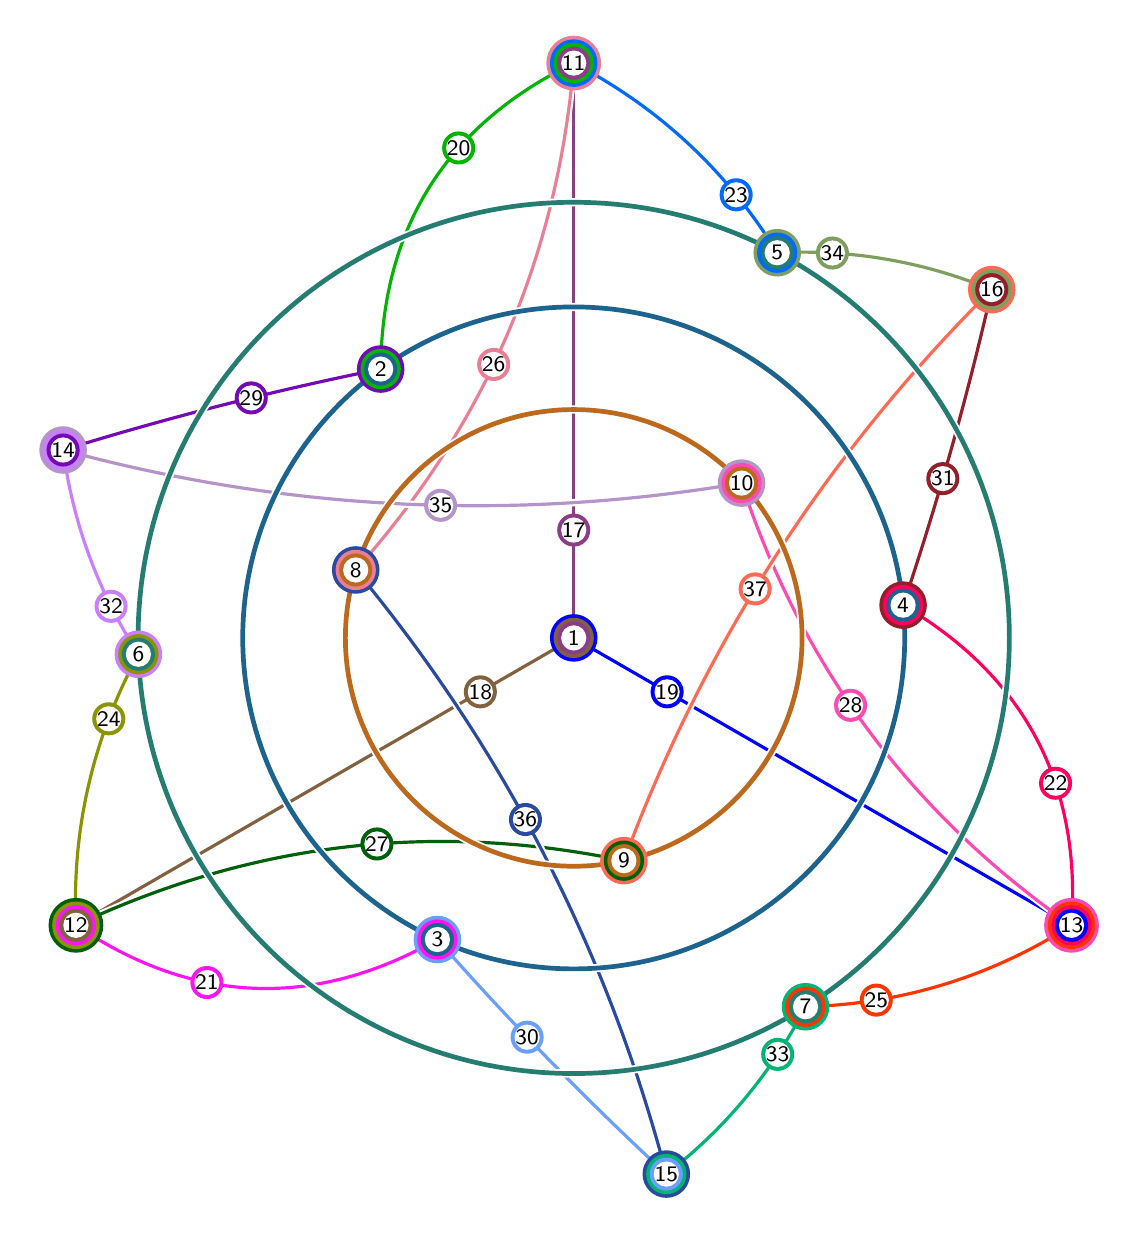
\begin{tikzpicture}[x=1cm,y=1cm]
% Layout has exact threefold symmetry, k -> k+1; vertex 1 is fixed.
% Coordinates are diagram positions, not the Hilbert-space vectors.
\coordinate (v1) at (0.0000000,0.0000000); % z
\coordinate (v2) at (-2.4516576,3.4144513); % M00
\coordinate (v3) at (-1.7311727,-3.8304234); % M01
\coordinate (v4) at (4.1828304,0.4159722); % M02
\coordinate (v5) at (2.5844238,4.8917486); % M10
\coordinate (v6) at (-5.5285905,-0.2076976); % M11
\coordinate (v7) at (2.9441666,-4.6840510); % M12
\coordinate (v8) at (-2.7685965,0.8628382); % M20
\coordinate (v9) at (0.6370585,-2.8290940); % M21
\coordinate (v10) at (2.1315381,1.9662558); % M22
\coordinate (v11) at (0.0000000,7.3000000); % P0
\coordinate (v12) at (-6.3219854,-3.6500000); % P1
\coordinate (v13) at (6.3219854,-3.6500000); % P2
\coordinate (v14) at (-6.4848807,2.3863586); % Q0
\coordinate (v15) at (1.1757932,-6.8092507); % Q1
\coordinate (v16) at (5.3090875,4.4228921); % Q2
\coordinate (v17) at (0.0000000,1.3694084); % A0
\coordinate (v18) at (-1.1859424,-0.6847042); % A1
\coordinate (v19) at (1.1859424,-0.6847042); % A2
\coordinate (v20) at (-1.4610288,6.2223311); % B00
\coordinate (v21) at (-4.6581824,-4.3764536); % B01
\coordinate (v22) at (6.1192112,-1.8458775); % B02
\coordinate (v23) at (2.0627119,5.6275810); % B10
\coordinate (v24) at (-5.9049841,-1.0274296); % B11
\coordinate (v25) at (3.8422722,-4.6001515); % B12
\coordinate (v26) at (-1.0167273,3.4728715); % B20
\coordinate (v27) at (-2.4992313,-2.6169474); % B21
\coordinate (v28) at (3.5159586,-0.8559241); % B22
\coordinate (v29) at (-4.0954594,3.0479105); % C00
\coordinate (v30) at (-0.5918382,-5.0707272); % C01
\coordinate (v31) at (4.6872977,2.0228167); % C02
\coordinate (v32) at (-5.8758527,0.4010894); % C10
\coordinate (v33) at (2.5905727,-5.2891825); % C11
\coordinate (v34) at (3.2852800,4.8880930); % C12
\coordinate (v35) at (-1.6906391,1.6838856); % C20
\coordinate (v36) at (-0.6129682,-2.3060792); % C21
\coordinate (v37) at (2.3036073,0.6221936); % C22
% context 4: {1,17,11}; z,A0,P0
\draw[sg/context,draw=ucA04,preaction={draw=white,line width=2.65pt}] (v1) -- (v11);
% context 5: {1,18,12}; z,A1,P1
\draw[sg/context,draw=ucA05,preaction={draw=white,line width=2.65pt}] (v1) -- (v12);
% context 6: {1,19,13}; z,A2,P2
\draw[sg/context,draw=ucA06,preaction={draw=white,line width=2.65pt}] (v1) -- (v13);
% context 7: {11,20,2}; P0,B00,M00
\draw[sg/context,draw=ucA07,preaction={draw=white,line width=2.65pt}] (v11) .. controls (-1.6178189,6.5099700) and (-2.4350381,5.2147871) .. (v2);
% context 8: {12,21,3}; P1,B01,M01
\draw[sg/context,draw=ucA08,preaction={draw=white,line width=2.65pt}] (v12) .. controls (-4.8288900,-4.6560572) and (-3.2986191,-4.7161984) .. (v3);
% context 9: {13,22,4}; P2,B02,M02
\draw[sg/context,draw=ucA09,preaction={draw=white,line width=2.65pt}] (v13) .. controls (6.4467088,-1.8539128) and (5.7336571,-0.4985887) .. (v4);
% context 10: {11,23,5}; P0,B10,M10
\draw[sg/context,draw=ucA10,preaction={draw=white,line width=2.65pt}] (v11) .. controls (1.0828326,6.7348007) and (1.9443072,5.9320502) .. (v5);
% context 11: {12,24,6}; P1,B11,M11
\draw[sg/context,draw=ucA11,preaction={draw=white,line width=2.65pt}] (v12) .. controls (-6.3739248,-2.4296398) and (-6.1094598,-1.2822056) .. (v6);
% context 12: {13,25,7}; P2,B12,M12
\draw[sg/context,draw=ucA12,preaction={draw=white,line width=2.65pt}] (v13) .. controls (5.2910922,-4.3051609) and (4.1651526,-4.6498446) .. (v7);
% context 13: {11,26,8}; P0,B20,M20
\draw[sg/context,draw=ucA13,preaction={draw=white,line width=2.65pt}] (v11) .. controls (-0.2047594,4.8454249) and (-1.1276249,2.6997043) .. (v8);
% context 14: {12,27,9}; P1,B21,M21
\draw[sg/context,draw=ucA14,preaction={draw=white,line width=2.65pt}] (v12) .. controls (-4.0938814,-2.6000393) and (-1.7742001,-2.3264040) .. (v9);
% context 15: {13,28,10}; P2,B22,M22
\draw[sg/context,draw=ucA15,preaction={draw=white,line width=2.65pt}] (v13) .. controls (4.2986408,-2.2453856) and (2.9018250,-0.3733004) .. (v10);
% context 16: {14,29,2}; Q0,C00,M00
\draw[sg/context,draw=ucA16,preaction={draw=white,line width=2.65pt}] (v14) .. controls (-5.1578542,2.7972430) and (-3.8134465,3.1399405) .. (v2);
% context 17: {15,30,3}; Q1,C01,M01
\draw[sg/context,draw=ucA17,preaction={draw=white,line width=2.65pt}] (v15) .. controls (0.1564436,-5.8654543) and (-0.8125450,-4.8725119) .. (v3);
% context 18: {16,31,4}; Q2,C02,M02
\draw[sg/context,draw=ucA18,preaction={draw=white,line width=2.65pt}] (v16) .. controls (5.0014106,3.0682113) and (4.6259915,1.7325713) .. (v4);
% context 19: {14,32,6}; Q0,C10,M11
\draw[sg/context,draw=ucA19,preaction={draw=white,line width=2.65pt}] (v14) .. controls (-6.3583368,1.4508121) and (-6.0395734,0.5861267) .. (v6);
% context 20: {15,33,7}; Q1,C11,M12
\draw[sg/context,draw=ucA20,preaction={draw=white,line width=2.65pt}] (v15) .. controls (1.9227283,-6.2318873) and (2.5121861,-5.5234874) .. (v7);
% context 21: {16,34,5}; Q2,C12,M10
\draw[sg/context,draw=ucA21,preaction={draw=white,line width=2.65pt}] (v16) .. controls (4.4356086,4.7810752) and (3.5273873,4.9373607) .. (v5);
% context 22: {14,35,10}; Q0,C20,M22
\draw[sg/context,draw=ucA22,preaction={draw=white,line width=2.65pt}] (v14) .. controls (-3.6435698,1.6140201) and (-0.7714302,1.4739859) .. (v10);
% context 23: {15,36,8}; Q1,C21,M20
\draw[sg/context,draw=ucA23,preaction={draw=white,line width=2.65pt}] (v15) .. controls (0.4240024,-3.9624340) and (-0.8907941,-1.4050711) .. (v8);
% context 24: {16,37,9}; Q2,C22,M21
\draw[sg/context,draw=ucA24,preaction={draw=white,line width=2.65pt}] (v16) .. controls (3.2195673,2.3484139) and (1.6622243,-0.0689148) .. (v9);
% context 1: {2,3,4}; M00,M01,M02
\draw[sg/base,draw=ucA01,preaction={draw=white,line width=3.0pt}] (0,0) circle[radius=4.2034632cm];
% context 2: {5,6,7}; M10,M11,M12
\draw[sg/base,draw=ucA02,preaction={draw=white,line width=3.0pt}] (0,0) circle[radius=5.5324905cm];
% context 3: {8,9,10}; M20,M21,M22
\draw[sg/base,draw=ucA03,preaction={draw=white,line width=3.0pt}] (0,0) circle[radius=2.8999339cm];
\HesseFCvertex{1}{ucA06/0.302000,ucA05/0.256000,ucA04/0.210000} % z
\HesseFCvertex{2}{ucA16/0.302000,ucA07/0.256000,ucA01/0.210000} % M00
\HesseFCvertex{3}{ucA17/0.302000,ucA08/0.256000,ucA01/0.210000} % M01
\HesseFCvertex{4}{ucA18/0.302000,ucA09/0.256000,ucA01/0.210000} % M02
\HesseFCvertex{5}{ucA21/0.302000,ucA10/0.256000,ucA02/0.210000} % M10
\HesseFCvertex{6}{ucA19/0.302000,ucA11/0.256000,ucA02/0.210000} % M11
\HesseFCvertex{7}{ucA20/0.302000,ucA12/0.256000,ucA02/0.210000} % M12
\HesseFCvertex{8}{ucA23/0.302000,ucA13/0.256000,ucA03/0.210000} % M20
\HesseFCvertex{9}{ucA24/0.302000,ucA14/0.256000,ucA03/0.210000} % M21
\HesseFCvertex{10}{ucA22/0.302000,ucA15/0.256000,ucA03/0.210000} % M22
\HesseFCvertex{11}{ucA13/0.348000,ucA10/0.302000,ucA07/0.256000,ucA04/0.210000} % P0
\HesseFCvertex{12}{ucA14/0.348000,ucA11/0.302000,ucA08/0.256000,ucA05/0.210000} % P1
\HesseFCvertex{13}{ucA15/0.348000,ucA12/0.302000,ucA09/0.256000,ucA06/0.210000} % P2
\HesseFCvertex{14}{ucA22/0.302000,ucA19/0.256000,ucA16/0.210000} % Q0
\HesseFCvertex{15}{ucA23/0.302000,ucA20/0.256000,ucA17/0.210000} % Q1
\HesseFCvertex{16}{ucA24/0.302000,ucA21/0.256000,ucA18/0.210000} % Q2
\HesseFCvertex{17}{ucA04/0.210000} % A0
\HesseFCvertex{18}{ucA05/0.210000} % A1
\HesseFCvertex{19}{ucA06/0.210000} % A2
\HesseFCvertex{20}{ucA07/0.210000} % B00
\HesseFCvertex{21}{ucA08/0.210000} % B01
\HesseFCvertex{22}{ucA09/0.210000} % B02
\HesseFCvertex{23}{ucA10/0.210000} % B10
\HesseFCvertex{24}{ucA11/0.210000} % B11
\HesseFCvertex{25}{ucA12/0.210000} % B12
\HesseFCvertex{26}{ucA13/0.210000} % B20
\HesseFCvertex{27}{ucA14/0.210000} % B21
\HesseFCvertex{28}{ucA15/0.210000} % B22
\HesseFCvertex{29}{ucA16/0.210000} % C00
\HesseFCvertex{30}{ucA17/0.210000} % C01
\HesseFCvertex{31}{ucA18/0.210000} % C02
\HesseFCvertex{32}{ucA19/0.210000} % C10
\HesseFCvertex{33}{ucA20/0.210000} % C11
\HesseFCvertex{34}{ucA21/0.210000} % C12
\HesseFCvertex{35}{ucA22/0.210000} % C20
\HesseFCvertex{36}{ucA23/0.210000} % C21
\HesseFCvertex{37}{ucA24/0.210000} % C22
\pgfresetboundingbox
\path[use as bounding box] (-6.9348807,-7.2592507) rectangle (6.7859111,7.7500000);
\end{tikzpicture}
% END INLINED FILE: figures/hesse37-figure.tex
}
\caption{Complete $3$-uniform hypergraph diagram of $H_{37}$ ($37$ rays, $24$ orthogonal triads, $72$ edges in $\C^3$). Bold circles denote $e_1,e_2,e_3$ ($\mathcal M_0,\mathcal M_1,\mathcal M_2$); the other $21$ smooth traces join core pairs through their unique completion rays $17,\ldots,37$. Concentric rings record incident context colors.}\label{h:fig:hesse37-hypergraph}
\end{figure*}

\begin{theorem}[Properties of $H_{37}$]\label{h:thm:main}
The hypergraph $H_{37}$ defined by Eqs.~\eqref{h:eq:ray-families}--\eqref{h:eq:contexts-M} satisfies:
\begin{enumerate}
\item It is linear with Berge girth five, $72$ edges, and $\omega(\Gamma(H_{37}))=3$; its triangles are precisely its $24$ contexts.
\item Equation~\eqref{h:eq:ray-families} defines an injective edge-faithful representation in $\C^3$, whereas $H_{37}$ admits \emph{no} injective orthogonal representation in $\R^3$.
\item Its chromatic numbers are $\chi(H_{37})=4>3=\chi_f(\Gamma(H_{37}))=\omega(\Gamma(H_{37}))$.
\item Its $24$ Boolean blocks paste into a $76$-event orthomodular lattice $L(H_{37})=\{0,1\}\cup\{a_i,a_i^\perp:1\le i\le 37\}$. Its full state space has $|\Sc(H_{37})|=153$ states and is order determining on $L(H_{37})$, with exact minimum state-family sizes $6$ for unital vertex separation, $7$ for separation of all $76$ events, and $18$ for order determination.
\end{enumerate}
\end{theorem}
\begin{proof}
(1)--(2) Zero patterns, magnitudes, and $\zeta$-phases distinguish all $37$ rays. Algebraic inner products confirm that $\ip{v_i}{v_j}=0$ holds strictly for the $24\binom{3}{2}=72$ context pairs: $\ip{M_{ak}}{M_{c\ell}}=1+\zeta^{c-a}(\zeta^{\ell-k}+\zeta^{2(\ell-k)})=0\iff(c=a,\ell\ne k)$; $P_j\perp M_{ak}\iff j=k$; $Q_j\perp M_{ak}\iff k=a+j$; $\ip{M_{c\ell}}{B_{ak}}=-2+\zeta^{a-c}(\zeta^{k-\ell}+\zeta^{2(k-\ell)})=0\iff(c,\ell)=(a,k)$; $\ip{M_{c\ell}}{C_{ak}}=1-2\zeta^{2a+k-c-\ell}+\zeta^{2k-c-2\ell}=0\iff(c=a,\ell=a+k)$; and unequal term magnitudes exclude orthogonalities among $A,B,C$. Uniqueness of cross-product completions in $\C^3$ excludes Berge $3$- and $4$-cycles, while $(\mathcal A_0,\mathcal B_{00},\mathcal M_0,\mathcal B_{01},\mathcal A_1)$ is a Berge $5$-cycle.

\phantomsection\label{h:sec:no-real-for}
To exclude any injective representation in $\R^3$, suppose unit $z\in\R^3$ and real $p_k,m_{ak}\in\R^3$ realize $\mathcal A_k,\mathcal B_{ak},\mathcal M_a$. If $m_{ak}\cdot z=0$, then $\{z,p_k,m_{ak}\}$ is an orthogonal basis of $\R^3$, and for $\ell\ne k$, $p_\ell\perp z$ and $m_{a\ell}\perp m_{ak}$ with $p_\ell\perp m_{a\ell}$ force $[p_\ell]=[m_{ak}]$ or $[m_{a\ell}]=[z]$. Hence $m_{ak}\cdot z\ne 0$. Rescaling so $m_{ak}\cdot z=1$ and choosing unit $u_k\in z^\perp\cap p_k^\perp$ gives $m_{ak}=z+t_{ak}u_k$ ($t_{ak}\in\R\setminus\{0\}$). Orthogonality of $\mathcal M_a$ yields $1+t_{ak}t_{a\ell}(u_k\cdot u_\ell)=0$ ($k\ne\ell$). Setting $q_k=t_{ak}/t_{0k}$ gives $q_0q_1=q_0q_2=q_1q_2=1$, whose only real solutions are $(q_0,q_1,q_2)=\pm(1,1,1)$. Thus at most two distinct bases $\mathcal M_a$ exist in $\R^3$, contradicting injectivity on the three bases $\mathcal M_0,\mathcal M_1,\mathcal M_2$.

(3) In any $3$-coloring with $c(z)=0$, $P_0,P_1,P_2\in\{1,2\}$ cannot be monochromatic (as $\mathcal M_a$ uses all three colors and $M_{ak}\sim P_k$). Up to symmetry $(c(P_0),c(P_1),c(P_2))=(2,1,1)$, forcing $c(M_{a0})=1$ and $(c(M_{a1}),c(M_{a2}))=(x_a,2-x_a)$ with $x_a\in\{0,2\}$. Since $N(Q_k)=\{M_{0k},M_{1,k+1},M_{2,k+2}\}$ avoids a color, $x_1=2-x_2$, $x_0=2-x_1$, $x_2=2-x_0$, impossible on a $3$-cycle. Thus $\chi(H_{37})=4$ (attained by $c(z)=0,c(M_{ak})=k,c(P_k)=c(Q_k)=3$). The $6$-state double cover $\mathcal R_6=\{s_2,s_{30},s_{73},s_{99},s_{109},s_{139}\}$ covers every vertex twice, giving $\chi_f(\Gamma(H_{37}))=3$.

\phantomsection\label{h:sec:order-determination}
(4) Each state is fixed by $t=(t_0,t_1,t_2)\in\Z_3^3$ with $s(M_{ak})=\mathbf 1_{k=t_a}$, $s(z)=\varepsilon\in\{0,1\}$, and independent bits on $U(t)=\Z_3\setminus\{t_0,t_1,t_2\}$ (for $\varepsilon=0$) and $W(t)=\Z_3\setminus\{t_a-a\}$, yielding $(1+2^{|U(t)|})2^{|W(t)|}$ states per $t$:
\begin{equation}\label{h:eq:state-count-breakdown}
\begin{array}{c|ccc}
\text{Class of }t\in\Z_3^3 & |\#t| & (|U(t)|,|W(t)|) & (1+2^{|U|})2^{|W|}\\\hline
(c,c,c) & 3 & (2,0) & 5\times 1=5\\
(c,c+1,c+2) & 3 & (0,2) & 2\times 4=8\\
(c,c+2,c+1) & 3 & (0,0) & 2\times 1=2\\
\text{Two equal entries} & 18 & (1,1) & 3\times 2=6
\end{array}
\end{equation}
and hence $|\Sc(H_{37})|=3\cdot5+3\cdot8+3\cdot2+18\cdot6=153$. Since $2^5-1=31<37$ and $2^6=64<76$, the explicit families $\Omega_6$ and $\Omega_7$ given in the supplement prove the minima $6$ and $7$. For order determination ($a_i\le a_j^\perp\iff i\sim j$), the $15$ nonorthogonal pairs in $D=\{P_0,P_1,P_2,Q_0,Q_1,Q_2\}$ require $15$ disjoint joint-one witnesses in $T\subset\Sc(H_{37})$ ($|T|=27$), and the $9$ pairs $\{z,C_{ak}\}$ require at least $2$ states outside $T$. Exhaustive bit-set verification over all $4{,}096\times 132=540{,}672$ candidate $17$-state families shows each meets at most $75$ of the $81$ minimal witness sets $W_{xy}$, whereas the $18$-state family $\Omega_{18}$ in the supplement meets all $81$ (Supplement Sec.~S3).
\end{proof}

By Proposition~\ref{prop:apex}, appending $d-3$ common apices to $H_{37}$ in $\C^d$ ($d\ge3$) gives faithful $d$-uniform hypergraphs with $|V|=d+34$, $|E|=24$, $\omega=d$, $\chi=d+1$, and $|\Sc|=d+150$.

An order-determining family represents the specified 76-event order, orthocomplements, and Boolean operations within listed contexts. It does not preserve arbitrary meets as set intersections: nonorthogonal atoms have meet zero although some states make both true. It is therefore not a Boolean-sublattice embedding of the full lattice, nor a claim of closure under every Hilbert operation. In particular, the minimum six-state separating family and the six-state uniform double cover solve different problems.

\subsection{Hyperplane obstruction, two-plane completion lemma, and canonical linear \texorpdfstring{$H_{65}$}{H65} in \texorpdfstring{$\R^4$}{R4}}

Appending a single apex $v_{26}=(0,0,0,1)^T\in\R^4$ to $H_{\YO}^{+}$ gives the $26$-ray, $16$-context non-linear suspension $H_{\YO}^{(4)}$ (Fig.~\ref{d:fig:hyo4}) with $\omega=4,\chi=5$, and $25$ unital separating states (Proposition~\ref{prop:apex}), but $|e\cap e'|=2$ ($g=2$).

\begin{figure*}[t]
\centering
\resizebox{.68\linewidth}{!}{%
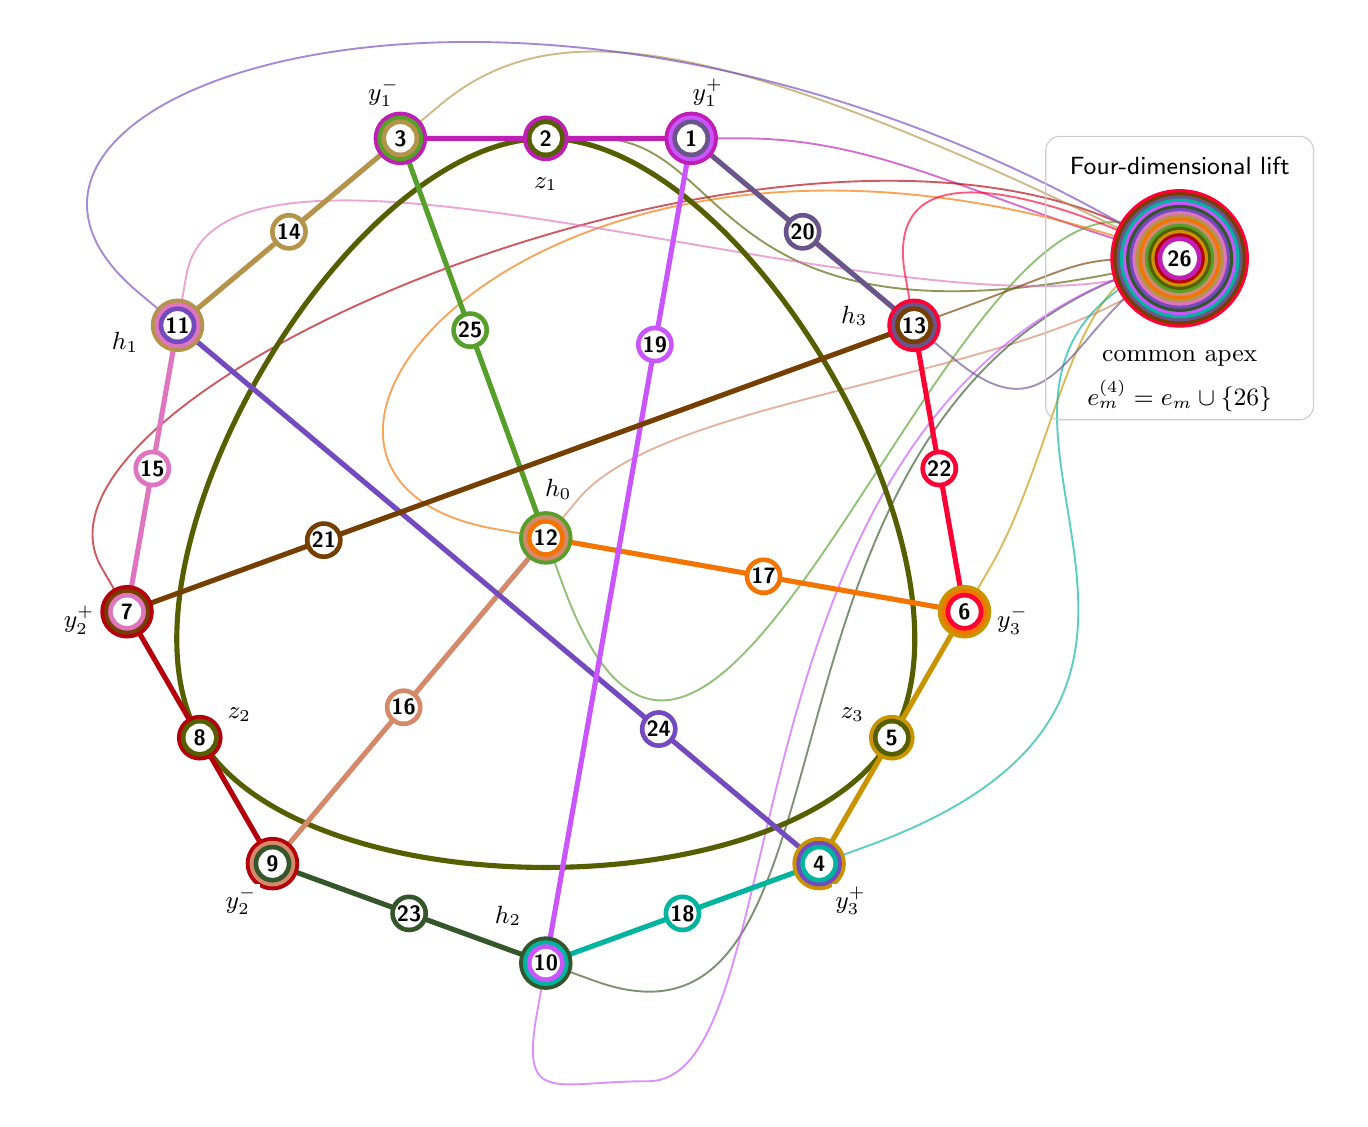
\begin{tikzpicture}[x=1cm,y=1cm]
\def\YOR{5.4}
\foreach \vertex/\angle in {1/70,3/110,11/150,7/190,9/230,10/270,4/310,6/350,13/30}{\coordinate (v\vertex) at (\angle:\YOR);}
\coordinate (v12) at (0,0);
\coordinate (v2) at ($(v1)!.5!(v3)$);\coordinate (v8) at ($(v7)!.5!(v9)$);\coordinate (v5) at ($(v4)!.5!(v6)$);
\foreach \vertex/\first/\last in {14/3/11,15/11/7,23/9/10,18/10/4,22/6/13,20/13/1}{\coordinate (v\vertex) at ($(v\first)!.5!(v\last)$);}
\foreach \vertex/\last in {25/3,16/9,17/6}{\coordinate (v\vertex) at ($(v12)!.52!(v\last)$);}
\foreach \vertex/\first/\last in {24/11/4,19/10/1,21/13/7}{\coordinate (v\vertex) at ($(v\first)!.75!(v\last)$);}
\coordinate (v26) at (8.05,3.55);\coordinate (YOgrayBefore) at ($(v2)+(-1,0)$);
\YOapexlink{1}{v2}{v1}{0.351939419}{1.326540885}{(5.550000,4.250000)}
\YOapexlink{2}{v8}{v7}{0.351939419}{1.813841619}{(4.050000,6.550000)}
\YOapexlink{3}{v5}{v6}{0.351939419}{1.326540885}{(6.650000,3.550000)}
\YOapexlink{4}{YOgrayBefore}{v2}{0.650000000}{2.450000000}{(2.050000,2.050000)}
\YOapexlink{5}{v25}{v12}{0.231481481}{2.368233618}{(5.550000,6.550000)}
\YOapexlink{6}{v16}{v12}{0.231481481}{0.872507123}{(6.650000,2.050000)}
\YOapexlink{7}{v17}{v12}{0.231481481}{1.655982906}{(0.050000,6.550000)}
\YOapexlink{8}{v14}{v3}{0.351939419}{1.326540885}{(2.050000,6.550000)}
\YOapexlink{9}{v15}{v11}{0.351939419}{1.813841619}{(5.550000,2.050000)}
\YOapexlink{10}{v24}{v11}{0.081484852}{0.582930092}{(0.050000,8.550000)}
\YOapexlink{11}{v23}{v10}{0.351939419}{2.517720456}{(2.050000,2.050000)}
\YOapexvia{12}{v19}{v10}{0.081484852}{0.231918424}{(0.100000,-6.900000)}{(1.300000,-6.900000)}{(3.300000,-6.900000)}{(2.050000,2.050000)}
\YOapexlink{13}{v18}{v4}{0.351939419}{3.600610974}{(4.050000,2.050000)}
\YOapexlink{14}{v20}{v13}{0.351939419}{1.326540885}{(6.650000,2.850000)}
\YOapexlink{15}{v21}{v13}{0.081484852}{0.307135210}{(6.650000,3.550000)}
\YOapexlink{16}{v22}{v13}{0.351939419}{1.326540885}{(6.650000,4.250000)}
\pgfmathsetmacro{\YObasisR}{\YOR*cos(20)}
\foreach \rotation in {0,120,240}{\begin{scope}[rotate=\rotation]\draw[YOtrace,YOctx4] (0,\YObasisR) .. controls ({-.5*\YObasisR},\YObasisR) and ({-(sqrt(3)/2+.25)*\YObasisR},{(-.5+.25*sqrt(3))*\YObasisR}) .. ({-sqrt(3)/2*\YObasisR},{-.5*\YObasisR});\end{scope}}
\YOline{1}{3}{2}{1}\YOline{2}{9}{8}{7}\YOline{3}{4}{5}{6}\YOline{5}{3}{25}{12}\YOline{6}{9}{16}{12}\YOline{7}{6}{17}{12}\YOline{8}{11}{14}{3}\YOline{9}{7}{15}{11}\YOline{10}{4}{24}{11}\YOline{11}{9}{23}{10}\YOline{12}{1}{19}{10}\YOline{13}{10}{18}{4}\YOline{14}{1}{20}{13}\YOline{15}{7}{21}{13}\YOline{16}{6}{22}{13}
\YOvertex{1}{1/.34,12/.29,14/.24}\YOvertex{2}{1/.29,4/.24}\YOvertex{3}{1/.34,5/.29,8/.24}\YOvertex{4}{3/.34,10/.29,13/.24}\YOvertex{5}{3/.29,4/.24}\YOvertex{6}{3/.34,7/.29,16/.24}\YOvertex{7}{2/.34,15/.29,9/.24}\YOvertex{8}{2/.29,4/.24}\YOvertex{9}{2/.34,6/.29,11/.24}\YOvertex{10}{11/.34,13/.29,12/.24}\YOvertex{11}{8/.34,9/.29,10/.24}\YOvertex{12}{5/.34,6/.29,7/.24}\YOvertex{13}{16/.34,14/.29,15/.24}\YOvertex{14}{8/.24}\YOvertex{15}{9/.24}\YOvertex{16}{6/.24}\YOvertex{17}{7/.24}\YOvertex{18}{13/.24}\YOvertex{19}{12/.24}\YOvertex{20}{14/.24}\YOvertex{21}{15/.24}\YOvertex{22}{16/.24}\YOvertex{23}{11/.24}\YOvertex{24}{10/.24}\YOvertex{25}{5/.24}
\foreach \angle/\symbol in {70/{y_1^+},110/{y_1^-},190/{y_2^+},230/{y_2^-},310/{y_3^+},350/{y_3^-}}{\node[YOlabel] at (\angle:6.02) {$\symbol$};}
\node[YOlabel,anchor=east] at ($(v11)+(-.45,-.22)$) {$h_1$};\node[YOlabel] at ($(v10)+(-.48,.60)$) {$h_2$};\node[YOlabel] at ($(v13)+(-.76,.12)$) {$h_3$};
\foreach \angle/\symbol in {90/{z_1},210/{z_2},330/{z_3}}{\node[YOlabel] at (\angle:{\YObasisR-.58}) {$\symbol$};}
\node[YOlabel] at (.16,.62) {$h_0$};
\draw[draw=black!20,rounded corners=5pt] (6.35,1.50) rectangle (9.75,5.10);
\node[font=\sffamily\small] at (8.05,4.72) {Four-dimensional lift};
\foreach \context/\radius in {16/.88,15/.84,14/.80,13/.76,12/.72,11/.68,10/.64,9/.60,8/.56,7/.52,6/.48,5/.44,4/.40,3/.36,2/.32,1/.28}{\fill[YOctx\context] (v26) circle[radius=\radius cm];}
\fill[white] (v26) circle[radius=.22cm];\node[YOnumber] at (v26) {26};
\node[font=\small] at (8.05,2.28) {common apex};\node[font=\small] at (8.05,1.80) {$e_m^{(4)}=e_m\cup\{26\}$};
\pgfresetboundingbox\path[use as bounding box] (-6.58,-7.12) rectangle (10.08,6.48);
\end{tikzpicture}}
\caption{The completed $25$-ray, $16$-context Yu--Oh hypergraph $H_{\YO}^{+}$ in $\R^3$ ($\omega=3,\chi=4$) and its non-linear $26$-ray, $16$-context apex suspension $H_{\YO}^{(4)}$ in $\R^4$ ($\omega=4,\chi=5,g=2$) obtained by adjoining the common orthogonal apex $v_{26}=(0,0,0,1)^T$ to every context.}\label{d:fig:hyo4}
\end{figure*}

\begin{proposition}[Hyperplane obstruction to linearity in $\F^4$]\label{d:prop:warmup}\label{d:prop:hyperplane-obstruction}
In any injective realization in $\PP(\F^4)$, if two contexts $e,e'$ each have three rays in a common $3$-dimensional hyperplane $W=z^\perp$, both must contain $[z]$; hence if $|e_W\cap e'_W|\ge1$, then $|e\cap e'|\ge2$, violating linearity.
\end{proposition}
\begin{proof}
Three mutually orthogonal rays in $W$ span $W$, forcing the fourth orthogonal ray of both $e$ and $e'$ to equal $[z]=W^\perp$.
\end{proof}

\begin{lemma}[Simultaneous two-plane completion in $\R^4$]\label{d:lem:plane-completion}
Let $V_{\mathrm{core}}\subset\Q^4\setminus\{0\}$ be a finite set of non-collinear rational vectors with $4$-element orthogonal base contexts $E_{\mathrm{base}}$ ($|C\cap C'|\le1$) and let all remaining orthogonal pairs be the bridge pairs $E_{\mathrm{bridge}}=\{e_1,\ldots,e_M\}$ ($e_m=\{u_m,v_m\}$, $L_m=\spanop(v_{u_m},v_{v_m})$, $P_m=L_m^\perp$) such that every core vertex lies in a base context or is a bridge endpoint.
\begin{enumerate}
\item The pairs $e_m$ can be simultaneously completed to $4$-bases $E_m=\{u_m,v_m,w_{m,1},w_{m,2}\}$ by fresh integer vectors $w_{m,1},w_{m,2}\in P_m\cap\Z^4$ forming a linear edge-faithful hypergraph $H$ if and only if
\begin{equation}\label{d:eq:span-condition}
\begin{aligned}
v_z&\notin L_m&& (z\in V_{\rm core}\setminus e_m),\\
P_\ell&\ne L_m&& (\ell\ne m).
\end{aligned}
\end{equation}
\item If $G_{\mathrm{core}}$ is $K_5$-free, then $\omega(\Gamma(H))=4$ and $\chi(H)=\max\{4,\chi(G_{\mathrm{core}})\}$.
\item If all $G_{\mathrm{core}}$-independent base supports $S_1,\ldots,S_N$ form a unital separating family on the core, and the zero-profiles $Z(e_m)=\{\alpha:S_\alpha\cap e_m=\varnothing\}$ are nonempty and pairwise distinct, the $\le 2N$ canonical extensions $s_{\alpha,\varepsilon}$ ($\varepsilon\in\{0,1\}$, setting $(s_{\alpha,\varepsilon}(w_{m,1}),s_{\alpha,\varepsilon}(w_{m,2}))=(1-\varepsilon,\varepsilon)$ when $\alpha\in Z(e_m)$ and $(0,0)$ otherwise) are unital and separating on $V(H)$.
\end{enumerate}
\end{lemma}
\begin{proof}
If $v_z\in L_m$ then $P_m\subset v_z^\perp$, and if $P_\ell=L_m$ then $P_\ell\perp P_m$, forcing extra orthogonalities. Conversely, given Eq.~\eqref{d:eq:span-condition}, an integer orthogonal basis $\{\eta_A,\eta_B\}\subset P_m\cap\Z^4$ defines the infinite family $w_{m,1}(a,b)=a\eta_A+b\eta_B$, $w_{m,2}(a,b)=-\|\eta_B\|^2b\eta_A+\|\eta_A\|^2a\eta_B$, avoiding the finitely many $1$-dimensional intersections $z^\perp\cap P_m$, $\R z\cap P_m$, and $P_m\cap L_r$ ($r>m$) inductively. Linearity, coloring extension, and distinctness of canonical vertex profiles follow from Proposition~\ref{prop:completion} and distinctness of $Z(e_m)$.
\end{proof}

% Styles for H65 diagram
\definecolor{ucA25}{HTML}{AA005F}\definecolor{ucA26}{HTML}{AA15FF}\definecolor{ucA27}{HTML}{35AAC9}\definecolor{ucA28}{HTML}{7F3F55}\definecolor{ucA29}{HTML}{0035E9}
\providecommand{\FCvertex}[2]{\foreach \diskcolor/\diskradius in {#2}{\fill[\diskcolor] (v#1) circle[radius=\diskradius cm];}\fill[white] (v#1) circle[radius=.160cm];\node[sg/number] at (v#1) {#1};}

\begin{figure*}[t]
\centering
\resizebox{.86\linewidth}{!}{%
\begin{tikzpicture}[x=1cm,y=1cm]
\coordinate (v1) at (-2,-2);\coordinate (v2) at (-5,5);\coordinate (v3) at (5,-5);\coordinate (v4) at (2,2);
\coordinate (v5) at (-5,-5);\coordinate (v6) at (-2,2);\coordinate (v7) at (2,-2);\coordinate (v8) at (5,5);
\coordinate (v9) at (-1.521690,0.927051);\coordinate (v10) at (1.800000,-0.860561);\coordinate (v11) at (-1.521690,-0.927051);
\coordinate (v12) at (0,7.3);\coordinate (v13) at (0.85,0);\coordinate (v14) at (0,2.333);\coordinate (v15) at (0,-2.333);\coordinate (v16) at (2.333,0);\coordinate (v17) at (-2.333,0);
\coordinate (v18) at (-1.7,6.518);\coordinate (v19) at (-3.35,5.759);\coordinate (v20) at (7.51031,2.131747);\coordinate (v21) at (7.443563,-1.627935);
\coordinate (v22) at (0.329875,-0.365);\coordinate (v23) at (-0.2045,-0.74);\coordinate (v24) at (1.172,0.56);\coordinate (v25) at (1.49975,1.13);
\coordinate (v26) at (-2.225,3.519815);\coordinate (v27) at (-3.575,4.239905);\coordinate (v28) at (0.665,2.222278);\coordinate (v29) at (1.325,2.112388);
\coordinate (v30) at (-0.8,-2.1998);\coordinate (v31) at (-1.4,-2.0999);\coordinate (v32) at (2.225,-3.519815);\coordinate (v33) at (3.6125,-4.259908);
\coordinate (v34) at (3.579823,-2.3375);\coordinate (v35) at (4.099888,-3.3125);\coordinate (v36) at (2.222278,0.665);\coordinate (v37) at (2.112388,1.325);
\coordinate (v38) at (-2.18981,-0.86);\coordinate (v39) at (-2.094905,-1.43);\coordinate (v40) at (-3.299787,1.8125);\coordinate (v41) at (-3.919865,2.975);
\coordinate (v42) at (-7.534215,1.984465);\coordinate (v43) at (-7.415219,-1.760849);\coordinate (v44) at (1.4,6.656);\coordinate (v45) at (2.7875,6.01775);
\coordinate (v46) at (0.116125,0.515);\coordinate (v47) at (-0.632,1.04);\coordinate (v48) at (1.12025,-0.47);\coordinate (v49) at (1.646375,-1.385);
\coordinate (v50) at (-0.515,2.247253);\coordinate (v51) at (-1.04,2.15984);\coordinate (v52) at (2.225,3.519815);\coordinate (v53) at (3.6125,4.259908);
\coordinate (v54) at (-2.225,-3.519815);\coordinate (v55) at (-3.6125,-4.259908);\coordinate (v56) at (0.665,-2.222278);\coordinate (v57) at (1.325,-2.112388);
\coordinate (v58) at (2.14985,-1.1);\coordinate (v59) at (2.07659,-1.54);\coordinate (v60) at (3.31979,1.85);\coordinate (v61) at (3.939868,3.0125);
\coordinate (v62) at (-3.31979,-1.85);\coordinate (v63) at (-3.939868,-3.0125);\coordinate (v64) at (-2.222278,0.665);\coordinate (v65) at (-2.112388,1.325);
\draw[sg/context,draw=ucA06] (v12)--(v2);\draw[sg/context,draw=ucA07] (0,7.3)..controls (10,9) and (8.5,-5)..(5,-5);
\draw[sg/context,draw=ucA08] (v13)--(v1);\draw[sg/context,draw=ucA09] (v13)--(v4);\draw[sg/context,draw=ucA10] (v14)--(v2);\draw[sg/context,draw=ucA11] (v14)--(v4);
\draw[sg/context,draw=ucA12] (v15)--(v1);\draw[sg/context,draw=ucA13] (v15)--(v3);\draw[sg/context,draw=ucA14] (v16)--(v3);\draw[sg/context,draw=ucA15] (v16)--(v4);
\draw[sg/context,draw=ucA16] (v17)--(v1);\draw[sg/context,draw=ucA17] (v17)--(v2);\draw[sg/context,draw=ucA18] (0,7.3)..controls (-10,9) and (-8.5,-5)..(-5,-5);
\draw[sg/context,draw=ucA19] (v12)--(v8);\draw[sg/context,draw=ucA20] (v13)--(v6);\draw[sg/context,draw=ucA21] (v13)--(v7);\draw[sg/context,draw=ucA22] (v14)--(v6);
\draw[sg/context,draw=ucA23] (v14)--(v8);\draw[sg/context,draw=ucA24] (v15)--(v5);\draw[sg/context,draw=ucA25] (v15)--(v7);\draw[sg/context,draw=ucA26] (v16)--(v7);
\draw[sg/context,draw=ucA27] (v16)--(v8);\draw[sg/context,draw=ucA28] (v17)--(v5);\draw[sg/context,draw=ucA29] (v17)--(v6);
\draw[sg/base,draw=ucA01,preaction={draw=white,line width=3pt}] (-5,5)..controls (-6.104569,3.895431) and (-4.761424,0.761424)..(-2,-2)..controls (0.761424,-4.761424) and (3.895431,-6.104569)..(5,-5)..controls (6.104569,-3.895431) and (4.761424,-0.761424)..(2,2);
\draw[sg/base,draw=ucA02,preaction={draw=white,line width=3pt}] (-5,-5)..controls (-6.104569,-3.895431) and (-4.761424,-0.761424)..(-2,2)..controls (0.761424,4.761424) and (3.895431,6.104569)..(5,5)..controls (6.104569,3.895431) and (4.761424,0.761424)..(2,-2);
\draw[sg/base,draw=ucA03,preaction={draw=white,line width=3pt}] (0,7.3)..controls (-0.50723,5.175684) and (-1.52169,1.593718)..(-1.52169,0.927051)..controls (-1.52169,0.260384) and (0.183333,0)..(0.85,0)..controls (1.516667,0) and (1.133333,-0.427228)..(1.8,-0.860561);
\draw[sg/base,draw=ucA04,preaction={draw=white,line width=3pt}] (0,2.333)..controls (0,1.883) and (-1.307492,2.163119)..(-1.52169,0.927051)..controls (-1.626103,0.324521) and (-1.626103,-0.324521)..(-1.52169,-0.927051)..controls (-1.307492,-2.163119) and (0,-1.883)..(0,-2.333);
\draw[sg/base,draw=ucA05,preaction={draw=white,line width=3pt}] (2.333,0)..controls (1.733,0) and (2.555418,-0.65741)..(1.8,-0.860561)..controls (0.831586,-1.120992) and (-0.478454,-1.147215)..(-1.52169,-0.927051)..controls (-2.43765,-0.733747) and (-1.733,0)..(-2.333,0);
\FCvertex{1}{ucA16/0.348,ucA12/0.302,ucA08/0.256,ucA01/0.21}\FCvertex{2}{ucA17/0.348,ucA10/0.302,ucA06/0.256,ucA01/0.21}\FCvertex{3}{ucA14/0.348,ucA13/0.302,ucA07/0.256,ucA01/0.21}\FCvertex{4}{ucA15/0.348,ucA11/0.302,ucA09/0.256,ucA01/0.21}
\FCvertex{5}{ucA28/0.348,ucA24/0.302,ucA18/0.256,ucA02/0.21}\FCvertex{6}{ucA29/0.348,ucA22/0.302,ucA20/0.256,ucA02/0.21}\FCvertex{7}{ucA26/0.266,ucA25/0.240,ucA21/0.214,ucA02/0.188}\FCvertex{8}{ucA27/0.348,ucA23/0.302,ucA19/0.256,ucA02/0.21}
\FCvertex{9}{ucA04/0.256,ucA03/0.21}\FCvertex{10}{ucA05/0.220,ucA03/0.191}\FCvertex{11}{ucA05/0.256,ucA04/0.21}
\FCvertex{12}{ucA19/0.394,ucA18/0.348,ucA07/0.302,ucA06/0.256,ucA03/0.21}\FCvertex{13}{ucA21/0.333,ucA20/0.299,ucA09/0.265,ucA08/0.231,ucA03/0.197}\FCvertex{14}{ucA23/0.317,ucA28/0.286,ucA11/0.255,ucA10/0.224,ucA04/0.193}\FCvertex{15}{ucA25/0.394,ucA24/0.348,ucA13/0.302,ucA12/0.256,ucA04/0.21}\FCvertex{16}{ucA27/0.394,ucA26/0.348,ucA15/0.302,ucA14/0.256,ucA05/0.21}\FCvertex{17}{ucA29/0.394,ucA28/0.348,ucA17/0.302,ucA16/0.256,ucA05/0.21}
\foreach \va/\vb/\col in {18/19/ucA06,20/21/ucA07,22/23/ucA08,24/25/ucA09,26/27/ucA10,28/29/ucA11,30/31/ucA12,32/33/ucA13,34/35/ucA14,36/37/ucA15,38/39/ucA16,40/41/ucA17,42/43/ucA18,44/45/ucA19,46/47/ucA20,48/49/ucA21,50/51/ucA22,52/53/ucA23,54/55/ucA24,56/57/ucA25,58/59/ucA26,60/61/ucA27,62/63/ucA28,64/65/ucA29}{\FCvertex{\va}{\col/0.21}\FCvertex{\vb}{\col/0.21}}
\node[sg/label,text=ucA01,anchor=south east] at (-4.7,5.65) {$C_1$};\node[sg/label,text=ucA02,anchor=north east] at (-4.7,-5.65) {$C_2$};\node[sg/label,text=ucA03,anchor=south] at (0,7.86) {$C_3$};\node[sg/label,text=ucA04,anchor=south] at (0,2.9) {$C_4$};\node[sg/label,text=ucA05,anchor=west] at (2.94,0) {$C_5$};
\end{tikzpicture}}
\caption{Canonical linear $4$-uniform hypergraph $H_{65}$ in $\R^4$ ($65$ rays, $29$ contexts, $174$ edges, $g=3,\omega=4,\chi=5$). Thick colored curves denote the five core contexts $C_1,\ldots,C_5$; the $24$ thinner lines denote the completed bridge contexts $E_1,\ldots,E_{24}$ carrying degree-one completion pairs $\{18,19\},\ldots,\{64,65\}$.}\label{d:fig:h65-hypergraph}
\end{figure*}

To construct a \emph{linear} $4$-uniform hypergraph in $\R^4$, we take the $17$-ray core $V_{\mathrm{core}}=\{1,\ldots,17\}\subset\{-1,0,1\}^4$, which is orthogonally equivalent to the $17$-ray Peres restriction of Haynes \emph{et al.}~\cite[pp.~8--9]{haynes2010orthogonal} via the orthogonal matrix
\begin{equation}\label{d:eq:haynes-transform}
T=\frac12\begin{pmatrix}
1&1&1&-1\\1&1&-1&1\\1&-1&1&1\\1&-1&-1&-1
\end{pmatrix},\qquad T^TT=I_4.
\end{equation}
consisting of the coordinate basis $C_1$, an even-parity Hadamard basis $C_2$, three odd-parity hub rays $9,10,11$, and the three binary bridge pairs $B_1=\{12,13\}$, $B_2=\{14,15\}$, $B_3=\{16,17\}$. The remaining base contexts are $C_3=\{9,10,12,13\}$, $C_4=\{9,11,14,15\}$ and $C_5=\{10,11,16,17\}$. Complete coordinates and all compatible supports are supplementary (Table~\ref{d:tab:bridge-neighbors}). Completing its $24$ uncovered bridge edges $e_m\in(C_1\cup C_2)\times(B_1\cup B_2\cup B_3)$ by fresh integer pairs $\{2m+16,2m+17\}\subset\{18,\ldots,65\}$ via Lemma~\ref{d:lem:plane-completion} yields $H_{65}=(V_{65},E_{29})$ (Fig.~\ref{d:fig:h65-hypergraph}, the corresponding supplemental table):
\begin{equation}\label{d:eq:h65-contexts}
\begin{aligned}
E_{29}&=\{C_1,\ldots,C_5\}\cup\{E_m:1\le m\le24\},\\
E_m&=\{u_m,v_m,2m+16,2m+17\}.
\end{aligned}
\end{equation}

% BEGIN INLINED FILE: tables/main-bridge-neighbors.tex
\begin{table}[t]
\centering\small\setlength{\tabcolsep}{3pt}
\caption{Bridge neighbors in the two core bases. The complete 24 state supports are supplementary.}\label{d:tab:bridge-neighbors}
\begin{tabular}{rp{.33\columnwidth}p{.33\columnwidth}}\toprule
$b$ & $N(b)\cap C_1$ & $N(b)\cap C_2$\\\midrule
$12$ & $\{2,3\}$ & $\{5,8\}$\\
$13$ & $\{1,4\}$ & $\{6,7\}$\\
$14$ & $\{2,4\}$ & $\{6,8\}$\\
$15$ & $\{1,3\}$ & $\{5,7\}$\\
$16$ & $\{3,4\}$ & $\{7,8\}$\\
$17$ & $\{1,2\}$ & $\{5,6\}$\\
\bottomrule\end{tabular}
\end{table}
% END INLINED FILE: tables/main-bridge-neighbors.tex


\begin{theorem}[Properties of $H_{65}$]\label{d:thm:h65}
The $65$-ray, $29$-context hypergraph $H_{65}$ satisfies:
\begin{enumerate}
\item It is linear ($g(H_{65})=3$) and edge-faithful in $\R^4$ ($174$ edges) with $\omega(\Gamma(H_{65}))=4$, and nonconformal ($13$ uncovered maximal triangles: $12$ bridge triangles plus $\{9,10,11\}$).
\item It has $\alpha(G_{\mathrm{core}})=4$, $\chi_f(\Gamma(H_{65}))=17/4=4.25>4$, and $\chi(H_{65})=5$.
\item Its core has $24$ compatible state supports $S_\alpha=\{i_1,i_2,h,b\}$ (Table~\ref{S-d:tab:app-h65-state-branches}), each missing $14$ bridges and yielding $|\Sc(H_{65})|=24\times 2^{14}=393{,}216$ states and $48$ canonical separating states.
\item Every $s\in\Sc(H_{65})$ obeys $s(9)+s(10)+s(11)=1$, so adjoining the fourth hub ray $q=(1,1,1,-1)^T$ forces $\widetilde s(q)=0$; moreover, $A_9=A_{16}\dot\cup A_{17}$ on all of $\Sc(H_{65})$, forcing the false atom-order implication $s(16)\le s(9)$ and collapsing the $1$-ray $[v_9]=[v_{16}-v_{17}]$ with the $2$-plane $\spanop(v_{16},v_{17})$.
\end{enumerate}
\end{theorem}
\begin{proof}
(1)--(2) No $K_4$ in $G_{\mathrm{core}}$ contains a bridge edge $\{u_m,v_m\}$, since $u_m\in C_a$ and $v_m\in B_k$ share only the second vertex of $N(v_m)\cap C_a$; this verifies $P_\ell\ne L_m$, and support-size / magnitude checks verify $v_z\notin L_m$ in Lemma~\ref{d:lem:plane-completion}. For any independent $I\subseteq V_{\mathrm{core}}$, $|I\cap C_1|\le1$ and $|I\cap C_2|\le1$. If $I\cap\{9,10,11\}\ne\varnothing$, $|I\cap(C_3\cup C_4\cup C_5)|\le2$ so $|I|\le4$; if $I\cap\{9,10,11\}=\varnothing$ and $I$ picks $(b_1,b_2,b_3)\in B_1\times B_2\times B_3$, even-parity triples cover $C_2$ and odd-parity triples cover $C_1$ (Table~\ref{d:tab:bridge-neighbors}), so again $|I|\le 3+1=4$. Thus $\alpha(G_{\mathrm{core}})=4$, $\chi_f\ge 17/4$ (matched by weights $1/8$ on the $24$ core states and $1/16$ on the $20$ remaining independent $4$-sets), and $\chi(H_{65})=5$. (3)--(4) By parity, no state can avoid $\{9,10,11\}$, giving $s(9)+s(10)+s(11)=1$, $3\times2\times2\times2=24$ core supports (Table~\ref{S-d:tab:app-h65-state-branches}), $24-10=14$ missed bridges per support, and $A_9=A_{16}\dot\cup A_{17}$.
\end{proof}
% END INLINED FILE: sections/05-hesse-and-4d.tex

% BEGIN INLINED FILE: sections/06-probabilities-and-ancestry.tex
\section{Event Order, Quantum Probabilities, and Nonextendable Weight}\label{sec:probabilities}

\subsection{Extendable state polytopes and the \texorpdfstring{$1/9$}{1/9} nonextendable weight bound on \texorpdfstring{$H_{17,10}$}{H17,10}}

For any context hypergraph $H$, the classical state polytope $\mathcal P(H)=\conv\Sc(H)$ and the extendable state polytope $\mathcal P_{\mathrm{ext}}(H)=\conv\Sc_{\mathrm{ext}}(H)$ satisfy $\mathcal P_{\mathrm{ext}}(H)\subseteq\mathcal P(H)$, with $p_u=p_v$ for all $p\in\mathcal P_{\mathrm{ext}}(H)$ whenever $u\sim_c v$ by Corollary~\ref{cor:hierarchy}. For $p\in\mathcal P(H)$, define its \emph{minimum nonextendable weight}
\begin{equation}\label{eq:weight}
\begin{aligned}
\eta_H(p)=\min_{\mu}\quad&\sum_{s\notin\mathcal S_{\mathrm{ext}}}\mu_s,\\
\text{subject to}\quad&p=\sum_{s\in\mathcal S}\mu_s s,\\
&\mu_s\ge0,\qquad\sum_s\mu_s=1.
\end{aligned}
\end{equation}

\begin{proposition}[Nonextendable weight lower bound]\label{prop:weight}
For any chromatically inseparable pair $u\sim_c v$ in $H$ and any $p\in\mathcal P(H)$, $\eta_H(p)\ge |p_u-p_v|$.
\end{proposition}
\begin{proof}
Every $s\in\Sc_{\mathrm{ext}}(H)$ satisfies $s(u)-s(v)=0$, while every $s\notin\Sc_{\mathrm{ext}}(H)$ satisfies $|s(u)-s(v)|\le1$, so $|p_u-p_v|\le\sum_{s\notin\Sc_{\mathrm{ext}}(H)}\mu_s|s(u)-s(v)|\le\sum_{s\notin\Sc_{\mathrm{ext}}(H)}\mu_s$.
\end{proof}

\begin{theorem}[Quantum preparation in $\mathcal P(H_{17,10})\setminus\mathcal P_{\mathrm{ext}}(H_{17,10})$]\label{thm:quantum}
In the real FOR of $H_{17,10}$ (the corresponding supplemental table), the pure quantum preparation along $r_{24}=(1,-1,2)^T$,
\begin{equation}\label{eq:rho}
\begin{aligned}
\rho_\star&=\frac16\begin{pmatrix}1&-1&2\\-1&1&-2\\2&-2&4\end{pmatrix},\\
p_i&=\Tr(\rho_\star P_i)=\frac{(r_{24}\cdot r_i)^2}{6\|r_i\|^2}.
\end{aligned}
\end{equation}
belongs to $\mathcal P(H_{17,10})$ via the exact five-state convex combination (state indices in the corresponding supplemental table)
\begin{equation}\label{eq:mixture}
p=\frac{1}{12}s_4+\frac{5}{36}s_9+\frac{1}{36}s_{10}+\frac{7}{12}s_{14}+\frac{1}{6}s_{17},
\end{equation}
yet satisfies $p_{24}=1$ and $p_{10}=8/9$ for the chromatically inseparable pair $(10,24)$, so
\begin{equation}\label{eq:quantum-gap}
p\notin\mathcal P_{\mathrm{ext}}(H_{17,10})\qquad\text{and}\qquad \eta_{H_{17,10}}(p)=\frac19.
\end{equation}
\end{theorem}
\begin{proof}
Direct evaluation of Eq.~\eqref{eq:mixture} on all $17$ vertices matches $p_i$ in Eq.~\eqref{eq:rho} (Table~\ref{S-tab:quantum}), with $r_{10}=(1,-1,1)^T$ giving $p_{10}=4^2/(6\cdot3)=8/9$. Since $10\sim_c 24$, Proposition~\ref{prop:weight} gives $\eta_{H_{17,10}}(p)\ge|1-8/9|=1/9$, which is attained in Eq.~\eqref{eq:mixture} because among $\{s_4,s_9,s_{10},s_{14},s_{17}\}$ precisely $s_4$ and $s_{10}$ are nonextendable, with total weight $1/12+1/36=1/9$.
\end{proof}

The exact support-and-weight certificate and the complete Born probability vector are given in the supplement. These tables are regenerated from the checked state inventory, rather than manually transcribed.

This preparation excludes only the coloring-completable model: its ordinary-state model is exhibited explicitly. Conversely, averaging the $d$ color classes of any admissible coloring gives the maximally mixed Born vector $1/d$, so the restricted obstruction is preparation dependent. The $H_{17,10}$ ordinary implication $s(10)\le s(24)$ also prevents order determination for distinct ray atoms; vertex separation and order representation must not be conflated.

\subsection{Order determination versus Born probabilities on \texorpdfstring{$H_{37}$, $H_{\YO}^{(4)}$, and $H_{65}$}{H37, HYO(4), and H65}}\label{h:sec:quantum-witness}\label{d:app:state-independence}

When $\chi(H)>d$ (Regime~I), $\mathcal P_{\mathrm{ext}}(H)=\varnothing$, and the relevant probability question is whether Born assignments $p_i(\rho)=\Tr(\rho\Pi_i)$ lie in $\mathcal P(H)=\conv\Sc(H)$ (Table~\ref{tab:probability-synthesis}).

\begin{corollary}[Order determination does not imply classical probability models]\label{cor:order-probabilities}
The $76$-event orthomodular lattice $L(H_{37})$ admits an order-determining state space $\Sc(H_{37})$ and a classical mixture for the maximally mixed state $I_3/3$, yet every $p\in\mathcal P(H_{37})$ satisfies the tight inequality
\begin{equation}\label{h:eq:pq-classical}
\mathcal C_{37}(p)=\sum_{k=0}^2\bigl[p(P_k)+p(Q_k)\bigr]\le 2,
\end{equation}
whereas the complex FOR of $H_{37}$ satisfies
\begin{equation}\label{h:eq:pq-projector-sum}
\sum_{k=0}^2(\Pi_{P_k}+\Pi_{Q_k})=\diag(3/2,3/2,3)=\frac32I_3+\frac32|e_3\rangle\langle e_3|,
\end{equation}
yielding $\mathcal C_{37}(\rho)=\frac32(1+\rho_{33})>2$ whenever $\rho_{33}>1/3$ (and $\mathcal C_{37}(|e_3\rangle\langle e_3|)=3$).
\end{corollary}
\begin{proof}
In the state parametrization of Theorem~\ref{h:thm:main}(4), every $t\in\Z_3^3$ has $|U(t)|+|W(t)|\le2$, establishing Eq.~\eqref{h:eq:pq-classical}, while summing the normalized projectors of $P_k,Q_k$ in Eq.~\eqref{h:eq:ray-families} using $1+\zeta+\zeta^2=0$ gives Eq.~\eqref{h:eq:pq-projector-sum}. Uniform weights $1/6$ on $\mathcal R_6$ reproduce $p_i(I_3/3)=1/3$.
\end{proof}

% BEGIN INLINED FILE: tables/main-probabilities.tex
\begin{table*}[t]
\centering\small\setlength{\tabcolsep}{3pt}
\caption{Event order and preparation-dependent probability models for the fixed realizations. Membership statements concern Born vectors $p(\rho)$; the restricted model is $\mathcal P_{\rm ext}$.}\label{tab:probability-synthesis}
\begin{tabular}{p{.14\textwidth}p{.26\textwidth}p{.26\textwidth}p{.26\textwidth}}\toprule
Configuration & Order determination & An ordinary-state model & A failed model or witness\\\midrule
$H_{17,10}$ & No: $s(10)\le s(24)$ is a false ray inclusion. & $P_{24}$ has an ordinary mixture. & $P_{24}\notin\mathcal P_{\mathrm{ext}}$; $\eta=1/9$.\\
Completed Yu--Oh & No. & No Born preparation lies in $\mathcal P$. & Every preparation gives $\sum_{10}^{13}p_i=4/3>1$.\\
$H_{37}$ & Yes on its specified 76-event lattice; 18 states minimal. & $I_3/3$ has a six-state mixture. & $\rho_{33}>1/3$ violates the $P,Q$ bound.\\
$H_{\YO}^{(4)}$ & No. & Pure apex $P_{26}$ has its singleton-state model. & Every $\rho\ne P_{26}$ violates the displayed bound.\\
$H_{65}$ & No: $s(16)\le s(9)$ is a false ray inclusion. & $(I_4-Q)/3$ has a model for all 65 rays. & $\Tr(\rho Q)>0$ violates the core sum bound.\\
\bottomrule\end{tabular}
\end{table*}
% END INLINED FILE: tables/main-probabilities.tex


In dimension four, the non-linear suspension $H_{\YO}^{(4)}$ obeys $\mathcal Y(p)=p_{26}+\sum_{i=10}^{13}p_i\le 1$ on $\mathcal P(H_{\YO}^{(4)})$, whereas $\sum_{i=10}^{13}\Pi_i=\frac43(I_4-\Pi_{26})$ gives $\mathcal Y(\rho)=1+(1-p_{26}(\rho))/3>1$ for every density operator $\rho\ne\Pi_{26}$~\cite{cabello2015sic}. For the canonical linear $H_{65}$, every $s\in\Sc(H_{65})$ has $4$ active core vertices, so every $p\in\mathcal P(H_{65})$ obeys $\sum_{i=1}^{17}p_i=4$. However, with $q=(1,1,1,-1)^T$ and $Q=qq^T/4$, direct summation gives
\begin{equation}\label{d:eq:core-projector-sum}
\sum_{i=1}^{17}\Pi_i=4I_4+Q\quad\Longrightarrow\quad \sum_{i=1}^{17}p_i(\rho)=4+\Tr(\rho Q),
\end{equation}
violating the classical bound $4$ whenever $\Tr(\rho Q)>0$ (including $I_4/4$, where the sum is $17/4=\chi_f$, and $\rho=Q$, where it is $5$). Nevertheless, on the orthogonal subspace $q^\perp$, the density operator $\rho_\star=(I_4-Q)/3$ has core Born probabilities $1/4$ on $C_1\cup C_2$, $1/3$ on $\{9,10,11\}$, and $1/6$ on $B_1\cup B_2\cup B_3$, and completion probabilities $r_{m,1}+r_{m,2}=7/12$. Choosing $\alpha\in\{1,\ldots,24\}$ uniformly and $\lambda\in[0,1]$ uniformly and setting $\varepsilon_m=\mathbf 1_{\{\lambda<\tau_m\}}$ with $\tau_m=\frac{12}{7}r_{m,2}\in\{4/9,5/11,6/11,5/9\}$ on the $14$ missed bridges of $S_\alpha$ gives $\mathbb E[s(w_{m,2})]=\frac{14}{24}\tau_m=r_{m,2}$, expressing $p(\rho_\star)\in\mathcal P(H_{65})$ as a convex mixture of at most $120$ states. Rotating $V_{\mathrm{core}}$ by $D_0=I_4,D_1=\diag(1,1,-1,-1),D_2=\diag(1,-1,1,-1),D_3=\diag(1,-1,-1,1)$ gives a fixed enlarged family with
\begin{equation}
\sum_{a,i}\Pi_i^{(a)}=17I_4,\qquad\sum_{a,i}p_i^{(a)}\le16\ \text{classically}.
\end{equation}
Each copy admits at most four true rays under geometric pair exclusions; repeated projectors are counted with multiplicity. The 24 distinct rays form the Peres set~\cite{peres-91}. This is an enlargement, not a state-independent test of the original 65 rays.

\section{KS Ancestry, Specified Parents, and Abstract versus Geometric States}\label{sec:ancestry}\label{sec:cabello-completion}\label{sec:cabello45}

\subsection{The KS ancestry hypothesis and abstract transverse extensions}

Motivated by the recurring parent structures of our examples, we formulate the \emph{KS ancestry hypothesis}: informally, ``any noncolorable ($\chi(H)>d$) configuration has a bigger KS ancestry.'' For realized ray configurations, an affirmative existence theorem holds even without the chromatic premise:

\begin{proposition}[Same-dimensional finite KS ancestry]\label{prop:ks-ancestry}
Every finite ray set $R\subset\PP(\F^d)$ ($\F\in\{\R,\C\}$, $d\ge3$) is a proper subset of a finite KS ray set $P\subset\PP(\F^d)$ whose orthogonality graph and full-basis hypergraph induce those on $R$, with every ray of $P$ in a complete context. Consequently, a finite graph $G$ has an injective edge-faithful realization in $\F^d$ if and only if $G$ is an induced subgraph of a finite KS orthogonality graph in $\F^d$.
\end{proposition}
\begin{proof}
Choose a finite full-basis KS set $K\subset\PP(\F^d)$~\cite{kochen1,cabello2005recursive}, orient $K$ by $U\in\mathrm{U}(d)$ (or $\mathrm{O}(d)$) so $UK\not\subseteq R$, and complete any uncovered rays of $R\cup UK$ to bases to obtain $P$. Any state on $P$ would restrict to a state on $UK$, a contradiction, and keeping the rays of $R$ fixed preserves all induced orthogonalities and full bases on $R$.
\end{proof}

By Theorem~\ref{m:thm:multipole}, $H_8$ has no injective realization, and $H_9,G_{32}$ have no ray assignment; none can embed into any $3$-dimensional geometric KS parent. For abstract hypergraphs, Lemma~\ref{lem:disjoint-states} yields a direct chromatic-to-stateless construction:

\begin{proposition}[Transverse chromatic-to-stateless extension]\label{prop:transverse}
For any finite $d$-uniform hypergraph $H=(V,E)$ ($d\ge3$), let $T(H)$ take $d-1$ disjoint copies $H^{(1)},\ldots,H^{(d-1)}$ and adjoin for each $v\in V$ a fresh vertex $w_v$ and the transverse context $T_v=\{v^{(1)},\ldots,v^{(d-1)},w_v\}$. Then $T(H)$ has $d|V|$ vertices, $(d-1)|E|+|V|$ contexts, is linear if $H$ is linear, and its two-valued states correspond bijectively to labeled strong $d$-colorings of $H$; in particular,
\begin{equation}\label{eq:transverse-equivalence}
\Sc(T(H))=\varnothing \quad\Longleftrightarrow\quad \chi(H)>d.
\end{equation}
\end{proposition}
\begin{proof}
A state $s\in\Sc(T(H))$ restricts to $d-1$ states on $H^{(k)}$ that are pairwise disjoint by $T_v$ (forcing $s(w_v)=1-\sum_{k=1}^{d-1}s(v^{(k)})$), which by Lemma~\ref{lem:disjoint-states} is equivalent to a strong $d$-coloring of $H$.
\end{proof}

In dimension $d=3$, any edge $u\sim v$ of $H$ creates a Berge $4$-loop $(u^{(1)},v^{(1)},u^{(2)},v^{(2)})$ in $T(H)$, excluding an injective realization in $\C^3$ by the common orthogonal-complement argument; thus $T(H)$ is an abstract construction. For $H_9$, $T(H_9)$ ($45$ vertices, $33$ contexts) is context-critical for statelessness on all $33$ contexts; for $H_{\YO}^{+}$, $T(H_{\YO}^{+})$ ($75$ vertices, $57$ contexts) is critical on all $32$ horizontal contexts and $12$ transverse contexts $v\in\{14,\ldots,25\}$, but remains stateless upon deleting $T_v$ for $v\in\{1,\ldots,13\}$ (Supplement Sec.~S3).

\subsection{Explicit inclusions in known KS parents and Cabello completions}\label{h:sec:comparison}

Beyond unrestricted existence, the following explicit unions use known KS components; the unions are not asserted to be previously named, smallest, or critical parents (explicit coordinate dictionaries and certificates in Supplement Secs.~S1--S3):
\begin{enumerate}
\item \emph{Bub's $49$-ray context-critical real parent of $H_{\YO}^{+}$:}
\begin{proposition}[Context-critical real parent of $H_{\YO}^{+}$]\label{prop:yo-real-parent}
Adjoining to $H_{\YO}^{+}$ the eight rays $(0,1,\pm2)$, $(0,2,\pm1)$, $(1,\pm2,0)$, $(2,\pm1,0)$ yields $33$ rays with $20$ bases and $16$ uncovered orthogonal pairs that eliminate all $24$ states of $H_{\YO}^{+}$. Completing those $16$ pairs yields the $49$-ray, $36$-context full-context Sch\"utte--Bub KS configuration~\cite{Pavicic-2005}, containing $H_{\YO}^{+}$ as an induced restriction, in which \emph{every} one of the $36$ contexts is critical for $\Sc=\varnothing$.
\end{proposition}
\item \emph{MUB-inventory parents of $H_{37}$:} In the $165$-ray, $130$-context MUB inventory~\cite{svozil-2025-MYOCHS} formed by three $69$-ray, $50$-context KS lineages $L_0,L_1,L_2$ (where each $L_a$ completes the $36$ uncovered pairs of Cabello's $33$-ray, $14$-basis KS set~\cite{Cabello2025}; by contrast, the two-gadget real/complex embedding construction of Harding and Salinas Schmeis~\cite[Thm.~2.6]{harding2025remarksIJTP} has $48$ rays, $32$ bases, $189$ context states, and $180$ geometric states), $H_{37}$ embeds as an induced restriction via the seed-index matrix $j(a,k)=\bigl(\begin{smallmatrix}1&2&3\\4&5&6\\7&9&8\end{smallmatrix}\bigr)$ mapping $z\leftrightarrow a_{1,1}$, $M_{ak}\leftrightarrow u_{j(a,k)}$, $P_k\leftrightarrow c_{1,k+1}$, $Q_k\leftrightarrow c_{2,k+1}$, $A_k\leftrightarrow b_{1,k+1}$, $B_{ak}\leftrightarrow d_{1,j(a,k)}$, $C_{ak}\leftrightarrow d_{2,j(a,a+k)}$. It lies in the $57$-ray, $40$-context intermediate spoke hypergraph ($297$ states) and in each $87$-ray, $64$-context KS union $H_{37}\cup L_a$.
\item \emph{Four-dimensional Peres and Cabello parents of $H_{\YO}^{(4)}$ and $H_{65}$:} Taking the union with Peres's $24$-ray set $P_{24}$~\cite{peres-91} gives a $40$-ray, $36$-context KS parent of $H_{\YO}^{(4)}$ ($|H_{\YO}^{(4)}\cap P_{24}|=10$; note that a single-apex lift of a $3$-dimensional KS set always retains the unique apex-one state) and a $72$-ray, $48$-context KS parent of $H_{65}$ ($|H_{65}\cap P_{24}|=17$). More economically:
\begin{proposition}[Three-ray KS extensions of $H_{65}$]\label{prop:h68-parent}
Adjoining $a=(1,0,0,1),b=(0,1,0,1),c=(0,0,1,1)$ to $H_{65}$ yields a $68$-ray, $35$-basis KS parent containing $H_{65}$ as an induced restriction and Cabello's $18$-ray, $9$-context parity proof $C_{18,9}$~\cite{cabello-96} ($C_3,C_4,C_5$ plus $D_1=\{2,3,12,a\},D_2=\{1,3,15,b\},D_3=\{1,2,17,c\},D_4=\{6,7,13,a\},D_5=\{6,8,14,b\},D_6=\{7,8,16,c\}$). Adjoining $(0,1,-1,0)$, $(1,0,-1,0)$, $(1,-1,0,0)$ instead yields a $68$-ray, $35$-basis KS parent containing a ray-critical $20$-ray, $11$-context parity proof $C_{20,11}$ ($11=4s(4)+4s(5)+2\sum_{i\ne4,5}s(i)$).
\end{proposition}
\begin{proof}
In $C_{18,9}$, summing $s$ over $C_3,C_4,C_5$ gives $3=2(s(9)+s(10)+s(11))+\sum_{k=12}^{17}s(k)$, so $s(12)+\cdots+s(17)$ is odd, whereas $D_1\oplus D_4,D_2\oplus D_5,D_3\oplus D_6$ give $s(12)+s(13)\equiv s(2)+s(3)+s(6)+s(7)$, $s(14)+s(15)\equiv s(1)+s(3)+s(6)+s(8)$, $s(16)+s(17)\equiv s(1)+s(2)+s(7)+s(8)\pmod 2$, summing to $0\pmod 2$. In $C_{20,11}$ (comprising $C_1,\ldots,C_5$ and six contexts on $\{1,\ldots,8,12,\ldots,17\}$ with $(0,1,-1,0)$, $(1,0,-1,0)$, $(1,-1,0,0)$), vertices $4,5$ have degree $4$ and the other $18$ vertices have degree $2$, so $11=4s(4)+4s(5)+2\sum_{i\ne4,5}s(i)$, an odd-equals-even contradiction; explicit states after deleting any single ray are certified in Supplement Sec.~S3.
\end{proof}
Both 68-ray presentations have 35 bases covering 192 of 195 geometric orthogonal pairs and context intersections of size up to two. They are not edge-faithful in the listed bases. The 72-ray Peres union covers all pairs; no size minimum or criticality of either full parent is asserted.

\item \emph{Faithful completion $C_{36,18}$ and abstract versus geometric states on $C_{45,21}$:}
\begin{corollary}[Faithful Cabello completion and vertex deletion]\label{cor:cabello36}
The $9$ uncovered orthogonal pairs of $C_{18,9}$ satisfy Eq.~\eqref{d:eq:span-condition}, so Lemma~\ref{d:lem:plane-completion} yields a linear edge-faithful $36$-ray, $18$-context KS hypergraph $C_{36,18}$ in $\R^4$ with $\omega=4,\chi=5$, and $\Sc=\varnothing$. Deleting one vertex (say $c$) and its two contexts from $C_{18,9}$ leaves $17$ rays, $7$ bases, $14$ uncovered pairs, and $12$ core states whose abstract completion $C_{45,21}$ has $\chi=5$ and $|\Sc_{\mathrm{ctx}}(C_{45,21})|=3{,}584$ unital separating context states ($24$ canonical). However, $v_{16}\in\spanop(v_1,v_2)$ and $v_{17}\in\spanop(v_7,v_8)$ violate Eq.~\eqref{d:eq:span-condition}, forcing four extra orthogonalities that reduce the geometric state space to $|\Sc_{\mathrm{geom}}(C_{45,21})|=2{,}048$ with $s(9)=s(16)=s(17)=0$, destroying unitality and separation (Table~\ref{tab:cabello-state-comparison}).
\end{corollary}
\begin{proof}
For $C_{18,9}$, the $9$ uncovered pairs are $6$ core bridges from $H_{65}$ plus $\{a,14\}$, $\{b,16\}$, $\{c,13\}$, which satisfy Eq.~\eqref{d:eq:span-condition} and complete via the corresponding supplemental table. Deleting $c,D_3,D_6$ leaves $12$ core supports ($8$ missing $8$ of the $14$ uncovered pairs and $4$ missing $7$), giving $8\cdot 2^8+4\cdot 2^7=3{,}584$ context states. Since $v_{16}=v_1+v_2$ and $v_{17}=\frac12(v_7-v_8)$, completing $\{1,2\}$ by $\{38,39\}$ and $\{7,8\}$ by $\{60,61\}$ forces $16\perp 38,39$ and $17\perp 60,61$; since $s(38)+s(39)=1$ whenever $s(16)=1$ and $s(60)+s(61)=1$ whenever $s(17)=1$, only the $4$ core supports with $s(9)=s(16)=s(17)=0$ survive in $\Sc_{\mathrm{geom}}(C_{45,21})$, yielding $4\cdot 2^9=2{,}048$ geometric states.
\end{proof}
\end{enumerate}

% BEGIN INLINED FILE: tables/main-geometric-states.tex
\begin{table*}[t]
\centering\small\setlength{\tabcolsep}{3pt}
\caption{Context and geometric state spaces in the four-dimensional examples. Linearity of the listed incidence structure does not imply edge-faithfulness.}\label{tab:cabello-state-comparison}
\begin{tabular}{p{.17\textwidth}rrrp{.48\textwidth}}\toprule
Configuration & $|V|/|E|$ & $|\Sc_{\mathrm{ctx}}|$ & $|\Sc_{\mathrm{geom}}|$ & Scope\\\midrule
$C_{18,9}$ & 18/9 & 0 & 0 & Nine uncovered geometric pairs; parity KS proof.\\
$C_{36,18}$ & 36/18 & 0 & 0 & Faithful linear completion.\\
$C_{45,21}$ & 45/21 & 3,584 & 2,048 & Four additional pairs destroy geometric unitality and separation.\\
$H_{65}$ & 65/29 & 393,216 & 393,216 & Edge-faithful; all context states respect the geometry.\\
\bottomrule\end{tabular}
\end{table*}
% END INLINED FILE: tables/main-geometric-states.tex


\section{Dependencies, counterexamples, and remaining questions}
The common dependency structure is incidence $\to$ states and colorings, followed by independent tests of geometry, event order, and quantum probabilities. A chromatic argument can be made on an abstract hypergraph; its operational interpretation requires a ray realization. Conversely, a realization does not select an ontic state family or a classical probability mixture. The exact-palette assumption adds a precise completion test at the level of whole truth assignments.

% BEGIN INLINED FILE: tables/main-limits.tex
% Analytical comparison; numerical examples checked against the electronic data.
\begin{table*}[t]
\centering\small\setlength{\tabcolsep}{4pt}
\caption{Logical boundaries of the integrated results. Each row prevents transfer of a conclusion between different assignment or representation problems.}\label{tab:logical-boundaries}
\begin{tabular}{p{.35\textwidth}p{.57\textwidth}}\toprule
Tempting unrestricted inference & Counterexample or necessary qualification\\\midrule
$\chi>d$ excludes states or ray realizations & Completed Yu--Oh has faithful real rays and 24 unital separating states.\\
Ordinary states separate $\Rightarrow$ colors separate & Faithful $H_{17,10}$ and $H_{21,13}$ have forced color identities.\\
Colors separate $\Rightarrow$ every state extends & The pentagon separates all vertex pairs but has one nonextendable state.\\
Vertex separation $\Rightarrow$ event-order determination & $H_{17,10}$ has $10\Rightarrow24$; $H_{65}$ has $16\Rightarrow9$ and ray--plane collapse.\\
Order determination $\Rightarrow$ all Born mixtures & Hesse's specified event order is represented, while $\rho_{33}>1/3$ violates the state inequality.\\
$\chi_f>d$ establishes fixed-measurement state independence & $H_{65}$ admits the Born model of $(I_4-Q)/3$ on all 65 rays.\\
Abstract stateless extension $\Rightarrow$ geometric KS parent & Closing a color-identical pair changes orthogonality; transverse four-loops exclude injective triadic geometry.\\
Generic KS ancestry explains the original chromatic gap & Unrestricted extension holds even for colorable sets and need not use the old rays essentially.\\\bottomrule
\end{tabular}
\end{table*}
% END INLINED FILE: tables/main-limits.tex




Table~\ref{tab:logical-boundaries} also explains why the probability and gadget examples carry different force. A one-way ordinary TITS already gives a symmetric color identity; a two-way purely chromatic identity requires counterstates in both truth directions. A ternary color exclusion may survive even when every pair can be equal. A strict inclusion $\mathcal P_{\rm ext}\subsetneq\mathcal P$ therefore need not be detectable through pair equalities alone.

Open problems concern global minimum faithful examples beyond the specified inventory, economical rational completions with fewer degree-one rays, residual-coloring certificates in dimensions above three, and geometric ancestry in which the retained rays are essential to the contradiction. The current statements establish existence and the recorded finite classifications, without asserting these stronger minima or essential-ancestry properties. All complete enumerations and the detailed verification scope remain in the supplement and electronic records.

\section{Conclusion}\label{sec:conclusion}

By unifying common-spectrum chromatic obstructions ($\chi(H)>d$) with exact-palette chromatic separability constraints ($\chi(H)=d$, $\Sc_{\mathrm{ext}}(H)\subsetneq\Sc(H)$), we have distinguished the requirements across spectral labelings, geometric ray realizations, orthomodular event representations, and quantum probability models. At the foundation, $\chi(H)>d$ obstructs a context-independent common $d$-element spectral labeling of maximal context observables, whereas the exclusion of an injective realization for $H_8$ and of every ray assignment for $H_9,G_{32}$ requires direct Hermitian projection forcing, correcting the earlier spectral argument for $G_{32}$~\cite{svozil-2021-chroma} and establishing four-quadrant independence even at Berge girth five. Within chromatically complete hypergraphs ($\chi(H)=d$), our completion criterion ($\chi(\Gamma(H)[V\setminus\supp s])\le d-1$) characterizes which context states fit into colorings and explains the specified examples of chromatic identities ($u\sim_c v$) and purely chromatic TIFS/TITS/ternary constraints ($H_{17,10},H_{21,13},D_{16,9},T_{19,11},W_{16,6}^{(4)}$) and yields a measurable $1/9$ nonextendable weight gap for a quantum ray preparation on $H_{17,10}$. In higher complexity, Hesse $H_{37}$ ($6/7/18$ OML minima) and our rational four-dimensional completion $H_{65}$ ($393{,}216$ states) demonstrate that neither exact order determination nor a fractional chromatic gap decides classicality for all Born preparations, while our KS ancestry theorems and Cabello completions ($C_{36,18},C_{45,21},H_{68,35}$) delineate unrestricted embedding from specified critical parents and geometric pair exclusions.
% END INLINED FILE: sections/06-probabilities-and-ancestry.tex

\begin{acknowledgments}
I thank Mohammad Hadi Shekarriz for valuable comments and suggestions. This research was funded in part by the Austrian Science Fund (FWF), Grant DOI \href{https://doi.org/10.55776/PIN5424624}{10.55776/PIN5424624}. The author acknowledges FWF and TU Wien Bibliothek for support through the Open Access Funding Programme. AI tools assisted with editorial work and computational checks. The author retains responsibility.
\end{acknowledgments}
\bibliographystyle{apsrev4-2}
\bibliography{C:/mytex/svozil}
\end{document}
